\documentclass[12pt]{caltech_thesis}
\usepackage[hyphens]{url}
\usepackage{lipsum}
\usepackage{graphicx}
\usepackage{xcolor}
\usepackage{hyperref}
\usepackage{orcidlink}
\usepackage{todonotes}
\usepackage{tabularx}
\usepackage{siunitx}
\usepackage{booktabs}
\usepackage{graphicx}
\usepackage{subcaption}
\usepackage{subcaption}
\usepackage{gensymb}
\usepackage{pdfpages}
\usepackage[utf8]{inputenc}
\usepackage{listings}
\usepackage{xcolor}
\usepackage[utf8]{inputenc}
\usepackage{tocloft}
\usepackage{caption} % Agrega el paquete caption
\usepackage{booktabs}
\usepackage{caption}
\captionsetup{labelsep=period}
\usepackage{adjustbox}
\usepackage{array}
\usepackage{makecell}
\usepackage{tocbibind}
\usepackage{etoc}
\usepackage[spanish]{babel}
\usepackage[utf8]{inputenc}  % Agrega este paquete para habilitar la codificación UTF-8


% Configura el entorno 'lstlisting' para usar 'Código' como etiqueta y una numeración distinta
\DeclareCaptionType{code}[Código][Índice de códigos]
\captionsetup[lstlisting]{labelsep=period}
\renewcommand\lstlistingname{Código}
\renewcommand\lstlistlistingname{Listado de Códigos}
\renewcommand{\arraystretch}{1.3}



\lstset{
    backgroundcolor=\color{white},
    basicstyle=\ttfamily,
    breaklines=true,
    frame=single,
    numbers=left,
    numberstyle=\tiny,
    language=C++, % Ajusta el lenguaje según tu caso
    showstringspaces=false,
}

% Configuración personalizada del estilo del código
\lstdefinestyle{mystyle}{
    backgroundcolor=\color{lightgray},     % Color de fondo
    basicstyle=\ttfamily,                 % Fuente
    breaklines=true,                     % Dividir líneas largas
    frame=single,                        % Marco alrededor del código
    numbers=left,                        % Números de línea a la izquierda
    numberstyle=\tiny\color{gray},       % Tamaño de los números de línea y color
    language=C++,                        % Lenguaje del código (ajusta según tu caso)
    keywordstyle=\color{blue},            % Estilo de las palabras clave
    commentstyle=\color{green!50!black},  % Estilo de los comentarios
    stringstyle=\color{red},              % Estilo de las cadenas de texto
    morekeywords={*,...},                % Puedes agregar más palabras clave aquí
    showstringspaces=false,              % No mostrar espacios en cadenas
    tabsize=4                            % Tamaño de tabulación
}

% Aplica el estilo personalizado
\lstset{style=mystyle}




\colorlet{linkcolor}{black} % Define el color de enlace como negro



%% Tentative: newtx for better-looking Times
\usepackage[utf8]{inputenc}
\usepackage[T1]{fontenc}
\usepackage{newtxtext,newtxmath}


\hypersetup{
  colorlinks=true,
  linkcolor=linkcolor,
  urlcolor=linkcolor,
  citecolor=linkcolor
  }


% Must use biblatex to produce the Published Contents and Contributions, per-chapter bibliography (if desired), etc.
\usepackage[
    backend=biber,natbib,
    % IMPORTANT: load a style suitable for your discipline
    style=ieee
]{biblatex}

% Name of your .bib file(s)
\addbibresource{example.bib}

\begin{document}


%Portada
% Do remember to remove the square bracket!
\title{Diseño y Simulación de un Sistema de Energía Basado en Componentes COTS para Globos de Gran Altitud en Ambiente Estratosférico }

\degreeaward{\text{Ingeniero Electricista}}
\mensaje{Tesis presentada por}
\author{Josué Romeo Aldana Aguilar}
\advisor{PhD. Jesús David González Llorente}
\reader{Dr. Luis Aarón Martínez}

% Degree to be awarded
\university{UNIVERSIDAD DON BOSCO}    % Institution name
\address{San Salvador, El Salvador}                     % Institution address
\unilogo{caltech.png}                                 % Institution logo
\copyyear{2023}  % Year (of graduation) on diploma
\defenddate{}          % Date of defense

\orcid{0000-0002-7686-5065}

%% IMPORTANT: Select ONE of the rights statement below.

%\todo[size=\footnotesize]{Choose one from the %choices in the source code!! And delete this %\texttt{todo} when you're done that. :-)}}
% \rightsstatement{All rights reserved except where otherwise noted}
% \rightsstatement{Some rights reserved. This thesis is distributed under a [name license, e.g., ``Creative Commons Attribution-NonCommercial-ShareAlike License'']}

%%  If you'd like to remove the Caltech logo from your title page, simply remove the "[logo]" text from the maketitle command
\maketitle[logo]
\makecopyright
%\maketitle

\title{Diseño y Simulación de un Sistema de Energía Basado en Componentes COTS para Globos de Gran Altitud en Ambiente Estratosférico }

\degreeaward{\text{Ingeniero Electricista}}
\mensaje{Decano de la Facultad de Ingeniería}
\author{Dr. Mario Guillermo Juárez Pérez}
\advisor{PhD. Jesús David González Llorente}
\reader{Dr. Luis Aarón Martínez}

% Degree to be awarded
\university{UNIVERSIDAD DON BOSCO}    % Institution name
\address{San Salvador, El Salvador}                     % Institution address
\unilogo{caltech.png} 
\maketitle[logo]


\title{Diseño y Simulación de un Sistema de Energía Basado en Componentes COTS para Globos de Gran Altitud en Ambiente Estratosférico }

\mensaje{}
\author{\textbf{EVALUACIÓN DEL TRABAJO DE GRADUACIÓN}}

\degreeaward{\text{Ingeniero Electricista}}
\advisor{PhD. Jesús David González Llorente}
\reader{Dr. Luis Aarón Martínez}
% Degree to be awarded
\university{UNIVERSIDAD DON BOSCO}    % Institution name
\address{San Salvador, El Salvador}                     % Institution address
\unilogo{caltech.png} 
\maketitle[logo]



% Abstract
\begin{abstract}
\hspace{1cm} Near space, spanning the altitude range between 20 and 100 km, remains an underexplored domain despite the increasing interest in space research. This region holds immense potential for advancing atmospheric physics, biology, environmental sciences, and other related fields. While the Low Earth Orbit (LEO) of nanosatellites fails to provide the required precision for these studies
and conventional aircraft rarely reach such altitudes, High-Altitude Balloons (HABs) emerge as a promising alternative. HABs operate at lower altitudes compared to nanosatellites, enabling exploration of critical areas of scientific interest, including the troposphere, tropopause, and stratosphere, while also offering more payload capacity.\\\\
 \hspace{1cm}This thesis primarily centers around the design of an EPS specifically optimized for short-duration missions typically lasting a few hours. Recognizing the critical role of the EPS in the overall functionality and effectiveness of other systems, this study applies the V-model methodology, following the project life cycle outlined in the NASA Systems Engineering Handbook. The EPS development life cycle encompasses phases such as needs/constraints analysis, system requirements identification,
architecture definition, design and implementation, system integration and testing, system verification and validation, culminating in the operation phase.

\hspace{1cm}This project is based on a systematic methodology and takes advantage of affordable commercial electronic components and open-source software, aiming to provide a low-cost solution. Relevant information, including laboratory tests, schematics, and algorithms, has been developed and documented, and made available in a GitHub repository. This not only offers an economical solution but also encourages collaboration and knowledge sharing within the scientific community. TThe results obtained, including circuit schematics, PCB designs, and programming logic flow charts, can enhance research capabilities in the Near-Space region and facilitate future scientific investigations.
\end{abstract}

%Agradecimientos
\begin{acknowledgements}

Quisiera expresar mi sincero agradecimiento a las siguientes personas e instituciones, quienes desempeñaron un papel fundamental en la realización de este trabajo de investigación:

\begin{itemize}
    \item \textbf{PhD. Jesús González:} A mi asesor de tesis, por su guía experta, paciencia y dedicación constante durante todo el proceso del trabajo de investigación. Su valioso asesoramiento ha sido crucial.

    \item \textbf{Familia:} Agradezco a mi familia por su apoyo incondicional y comprensión durante el tiempo dedicado a este trabajo. Especialmente quiero expresar mi gratitud a mis padres, cuyo apoyo ha sido fundamental. También dedico este trabajo a la memoria de mi abuelo, que en paz descanse, y que a lo largo de mi vida ha sido un ejemplo inspirador que ha guiado mis intereses de manera acertada.

    \item \textbf{Observatorio Micro-Macro (OMM):} Agradezco al Observatorio Micro-Macro, y especialmente a su directora, Brisa Terezón, por proporcionarme un espacio dentro del proyecto de investigación estudiantil StratoBalloon, al cual pertenece esta tesis. Es dentro de este marco que se llevará a cabo la implementación y desarrollo del diseño presentado en este trabajo.

    \item \textbf{Amigos y Colegas:} Quiero expresar mi agradecimiento a todos aquellos amigos y colegas que, de una u otra manera, contribuyeron directa o indirectamente a este trabajo. Sus aportes fueron invaluables y enriquecieron significativamente el desarrollo de la investigación.

\end{itemize}

A todos ellos, mi más profundo agradecimiento por ser parte integral de este viaje académico y por su contribución a la culminación exitosa de este trabajo de tesis.

\end{acknowledgements}


\newpage % Salto de página

\newpage % Salto de página adicional

% Eliminar la entrada del índice general en sí mismo

\addtocontents{toc}{\protect\setcounter{tocdepth}{-10}}
% Generar las listas de figuras, tablas y listados de código

\pagestyle{empty} % Desactiva la numeración de página

\tableofcontents

\pagestyle{plain} % Restaura la numeración de página normal

\listoffigures
\listoftables
\lstlistoflistings



% Restaurar el nivel de profundidad por defecto para la tabla de contenidos principal
\addtocontents{toc}{\protect\setcounter{tocdepth}{2}}

% Nomenclatura
\printnomenclature[4cm]
\makenomenclature


\nomenclature{BMS}{Battery Management System}
\nomenclature{BP}{Boost Power}
\nomenclature{BTMS}{Battery Thermal Management System}
\nomenclature{BTS}{Battery Charge-Discharge Testing Software}
\nomenclature{C/D}{Charge-Discharge}
\nomenclature{CC}{Constant Current}
\nomenclature{CMB}{Cosmic Microwave Background}
\nomenclature{COTS}{Commercial-Off-The-Shelf}
\nomenclature{CTR}{Compensated Temperature Range}
\nomenclature{CV}{Constant Voltage}
\nomenclature{D-C}{Discharge-Charge}
\nomenclature{DAQ}{Data Acquisition}
\nomenclature{DC}{Direct Current}
\nomenclature{DOD}{Depth of discharge}
\nomenclature{EPS}{Electrical Power System}
\nomenclature{ESA}{European Space Agency}
\nomenclature{GFS}{Global Forecast System}
\nomenclature{GNSS}{Global navigation satellite system}
\nomenclature{GUI}{Graphical User Interface}
\nomenclature{HAB}{High Altitude Balloon}
\nomenclature{IEC}{International Electrotechnical Commission}
\nomenclature{IMU}{Inertial Measurement Unit}
\nomenclature{ISA}{International Standard Atmosphere}
\nomenclature{LDO}{Low-dropout regulator}
\nomenclature{LEO}{Low-Earth Orbit}
\nomenclature{LIB}{Lithium-Ion Battery}
\nomenclature{MOSFET}{Metal Oxide Silicon Field Effect Transistors}
\nomenclature{NASA}{National Aeronautics and Space Administration}
\nomenclature{NIST}{National Institute of Standards and Technology}
\nomenclature{NOAA}{National Oceanic and Atmospheric Administration}
\nomenclature{OCV}{Open-Circuit Voltage}
\nomenclature{OMM}{Observatorio Micro Macro}
\nomenclature{PCB}{Printed Circuit Board}
\nomenclature{RTD}{Resistance Temperature Detector}
\nomenclature{SOC}{State of Charge}
\nomenclature{SOH}{State of Health}
\nomenclature{SPICE}{Simulation Program with Integrate Circuit Emphasis}
\nomenclature{STEM}{Science, technology, engineering, and mathematics}
\nomenclature{UART}{Universal Asynchronous Receiver Transmitter}
\nomenclature{USB}{Universal Serial Bus}
\nomenclature{VDA}{Vapor-Deposited Aluminum}

% CUERPO DEL DOCUMENTO
\mainmatter


%Capítulos
%INTRODUCCION
\chapter{Introducción}

\section{Planteamiento del problema}
\vspace{1 cm}

Los \emph{High Altitude Balloon} (HAB) se perfilan como herramientas efectivas y de bajo costo para instituciones que dan sus primeros pasos en la exploración espacial. Fabricados comúnmente con materiales económicos como el látex, estos globos permiten simular condiciones espaciales en misiones de corta duración, generalmente de unas pocas horas \cite{Saad2015}. Es crucial destacar que los HAB representan una opción inicial y asequible. A medida que las instituciones educativas avanzan en sus investigaciones, pueden acceder a plataformas más sofisticadas y especializadas.

En los Estados Unidos, instituciones como \emph{The National Weather Service}, en conjunto con la \emph{National Oceanic and Atmospheric Administration} (NOAA), lanzan diariamente múltiples HABs con el propósito de obtener información atmosférica \cite{noaa_upperair, noaa_radiosondes}. Además, en el ámbito científico, especialmente en astronomía, se han utilizado para experimentos como BOOMERanG, destinado a mapear el fondo cósmico de microondas (CMB) desde el Polo Sur. Asimismo, en 2017, 52 equipos de 30 estados diferentes colaboraron para el lanzamiento masivo de HABs y obtener imágenes en tiempo real y de alta calidad durante el eclipse solar total del 21 de agosto \cite{Jarrell2017}.

El desarrollo tecnológico en torno a los HABs es activo, incluso con diseños destinados a ser utilizados más allá de nuestro planeta, como el caso del VAB-X, un modelo propuesto para estudiar imágenes mediante vuelos sostenidos en la atmósfera de Venus \cite{Bugga2022}.

Actualmente, la NASA lidera el desarrollo de tecnología para globos científicos. Durante más de 30 años, el \emph{NASA Balloon Program} ha proporcionado plataformas de globos para investigaciones científicas y tecnológicas, logrando descubrimientos significativos que han contribuido a nuestro entendimiento de la Tierra, el sistema solar y el universo.

\newpage

Los HAB permiten realizar experimentos científicos en la estratosfera, aproximadamente a una altura de 30 km sobre la superficie terrestre, representando una oportunidad valiosa para países de Latinoamérica que aún no han incursionado en la exploración espacial, como es el caso de El Salvador \cite{latam}. A diferencia de los proyectos con cohetes y nanosatélites, los HAB son más asequibles, convirtiéndolos en una opción prometedora \cite{Jarrell2017}.

La necesidad de un sistema eléctrico de potencia (EPS, por sus siglas en inglés \textit{Electrical Power System}) eficiente y confiable es crítica para garantizar el funcionamiento de los instrumentos a bordo.

Un EPS se encarga de proveer, almacenar, acondicionar, controlar y distribuir la potencia eléctrica necesaria. Su diseño implica considerar aspectos como la fuente de energía, la capacidad de almacenamiento, el consumo, el voltaje, la corriente, la protección y la regulación.

Este proyecto de investigación aborda el diseño y simulación de un EPS adaptado a las condiciones específicas de misiones de globos de gran altitud. Se toma como referencia el estándar \emph{CubeSat}, ampliamente utilizado en nanosatélites, con el objetivo de adaptar sus principios de funcionamiento. La implementación eficiente de sistemas basados en componentes \emph{Commercial off-the-shelf} (COTS) y soluciones probadas plantea desafíos, como la falta de integración óptima y posibles conflictos de interoperabilidad. En este contexto, se destaca la necesidad de desarrollar un enfoque que permita una implementación más eficaz, acelerando el proceso de desarrollo y reduciendo los riesgos asociados.

Este proyecto contribuye a la confiabilidad de futuras investigaciones y pruebas en la estratosfera, y ocurre en el contexto de la misión StratoBalloon del Observatorio Micro-Macro (OMM). Se adopta el modelo V como metodología, debido a que es el ciclo de proyectos aprobado por la NASA \cite{NASA2016}. El proyecto se divide en las siguientes etapas: definición de requisitos, diseño conceptual, diseño detallado, implementación, verificación, validación y operación.

Hasta la fecha actual, año 2023, el registro de este tipo de proyectos en El Salvador es escaso, con un enfoque predominantemente recreativo a nivel aficionado \cite{NC}, a excepción de una publicación en una conferencia centroamericana \cite{Reyes2022} por parte de miembros del proyecto universitario al que pertenece esta tesis. Durante la búsqueda bibliográfica realizada, se ha constatado la ausencia de otras investigaciones sobre sistemas de energía para HAB a nivel nacional y regional.


\newpage
\section{Motivación del trabajo}
\vspace{1 cm}
La región de \emph{Near-Space}, situada a altitudes comprendidas entre los 20 y 100 kilómetros, alberga un vasto potencial para la investigación en diversas disciplinas científicas, como la física atmosférica, la biología y las ciencias ambientales. No obstante, enfoques convencionales, tales como nanosatélites en órbita terrestre baja (LEO, por sus siglas en inglés \emph{Low Earth Orbit}) y aeronaves tradicionales, se ven limitados en su capacidad de explorar esta región. En este contexto, los HABs emergen como una prometedora alternativa para llevar a cabo experimentos científicos.

La realización de proyectos que involucran sondas HAB no solo conlleva un potencial científico de relevancia, sino que también posee un significativo valor en el ámbito educativo. Esto se debe a que permite a los estudiantes participar en actividades de investigación, aplicar conocimientos teóricos mediante la práctica y fortalecer su capacidad para abordar desafíos multidisciplinarios. Además, estas misiones brindan a las instituciones educativas la oportunidad de incursionar en el sector aeroespacial, adquirir experiencia en el desarrollo de misiones espaciales y establecer colaboraciones tanto a nivel nacional como internacional.

Bajo este panorama, en el Observatorio Micro Macro se desarrolla una misión de globo metereológico, StratoBalloon, un desafío tecnológico a trabajar con un equipo multidisciplinario estudiantil.

Dentro de los componentes electrónicos que conforman una sonda HAB, el sistema de energía o EPS, desempeña un papel crítico en el funcionamiento y la eficacia de la misión espacial en su conjunto.

La relevancia y originalidad de este trabajo radica en el desarrollo del primer sistema de energía de bajo costo destinado a sondas HAB en nuestro país, con enfoque particular a la misión StratoBalloon. A través de la utilización de componentes electrónicos comerciales disponibles (COTS), la implementación de software de código abierto, simulaciones basadas en el modelo atmosférico GFS y el estándar atmosférico ISA, la concepción de arquitecturas lógicas y físicas, listas de verificación y una exhaustiva documentación, se consolida la propuesta de diseño del sistema EPS en este proyecto de investigación.

\newpage

\section{Objetivos de la investigación}
\vspace{1 cm}
\subsection{Objetivo General}
Diseñar un Sistema Eléctrico de Potencia (EPS) eficiente y confiable para misiones de corta duración en Globos de Gran Altitud (HAB), haciendo uso de componentes electrónicos comerciales disponibles (COTS) y software de código abierto.

\subsection{Objetivos Específicos}
\begin{enumerate}
    \item Determinar las condiciones ambientales aproximadas que caracterizan las misiones de HAB a la estratósfera, a una altitud de 30 kilómetros. 

    \item Establecer los requisitos eléctricos y energéticos necesarios para la misión, teniendo en cuenta los sistemas de navegación, telemetría y carga útil de la misión StratoBalloon.

    \item Diseñar tanto la arquitectura lógica como la física del EPS, con el propósito de identificar y seleccionar los componentes electrónicos y baterías más apropiados, considerando las condiciones de operación específicas de las misiones de HAB.

    \item Elaborar un plan de pruebas completo destinado a la verificación y validación del EPS de una sonda HAB, asegurando su correcto funcionamiento y confiabilidad en el entorno de la misión.
\end{enumerate}
\newpage


\section{Aspectos a considerar}
\vspace{1 cm}

\subsection{Alcance}

El alcance de la investigación es diseñar un sistema de energía eléctrica eficiente y confiable para misiones de corta duración en \emph{High Altitude Balloons} (HAB), que pueda alcanzar una altura de 30 km sobre el nivel del mar. Se utilizarán componentes \emph{Commercial Off-The-Shelf}  (COTS) y software libre para reducir los costos de fabricación y fomentar la colaboración en la comunidad. 

\subsection{Limitaciones}
\begin{enumerate}
    \item Recursos limitados: La disponibilidad de materiales y los costos asociados a las pruebas de laboratorio dependen de los fondos disponibles en el proyecto StratoBalloon y del respaldo proporcionado por la Escuela de Ingeniería Eléctrica.

    \item Tiempo: el período para desarrollar el proyecto de investigación es aproximadamente de 16 semanas, el uso de equipo o laboratorio está sujeto a terceros, lo cual podría incluso limitar el número de experimentos. De igual forma, la importación de componentes necesarios para las pruebas podría atrasar el desarrollo de la investigación.

    \item Pruebas en laboratorio: Las pruebas que se realicen idealmente deben simular las condiciones ambientales que se experimentarían en una sonda de HAB en trayectoria hacia la estratósfera. Es posible que sea difícil replicar estas condiciones con precisión en un laboratorio, o este no cuente con equipo adecuado para realizarlas, lo que podría afectar los resultados obtenidos.

    \item Simulaciones: Aunque el modelo \emph{Global Forecast System} (GFS) desarrollado por la \emph{National Oceanic and Atmospheric Administration} (NOAA) es una referencia útil para la obtención de datos atmosféricos y simulación de trayectorias, es importante tener en cuenta que este modelo también tiene limitaciones y puede no ser completamente preciso en todas las situaciones. De igual forma, el modelo atmosférico ISA.
\end{enumerate}


\newpage


\section{Ruta de la Tesis}

El contenido de esta tesis se divide en ocho capítulos.

En el Capítulo 1, se introduce el tema de investigación, se plantea el problema, se establecen los objetivos, el alcance y las limitaciones.

En el Capítulo 2, se revisa el estado del arte de los sistemas eléctricos de potencia (EPS) en la industria aeroespacial y las metodologías para su diseño.

En el Capítulo 3, se identifican las necesidades y restricciones que condicionan el diseño de un EPS para \emph{BalloonSat}, como las condiciones ambientales, el presupuesto energético, y las limitaciones de masa y volumen. También se resumen los requisitos que debe cumplir el sistema.

En el Capítulo 4, se define la arquitectura del EPS a nivel de bloques funcionales, desde el nivel 0 hasta el nivel 2, especificando las entradas, salidas y funciones de cada bloque.

En el Capítulo 5, se detalla el diseño e implementación del sistema, describiendo los componentes seleccionados y las capacidades desarrolladas para cada bloque. Se abordan aspectos como el microcontrolador, el \emph{datalogger}, la etapa de potencia, la instrumentación, las baterías, el cargador, la regulación de voltaje y los dispositivos de protección eléctrica.

En el Capítulo 6, se presenta la integración de los sistemas, explicando cómo se conectan los componentes entre sí y cómo se realiza el control y la comunicación del sistema. También se describen las pruebas realizadas para verificar el correcto funcionamiento del sistema integrado.

El Capítulo 7 consta de las listas de validación y verificación del sistema.

Finalmente, en el capítulo 8 se resumen los resultados de este trabajo de grado y se ofrecen recomendaciones para futuros trabajos relacionados.








%Here's an endnote.\endnote{Endnotes are notes that you can use to explain text in a document.}
% FIN INTRODUCCIÓN
\chapter{Antecedentes}
En el ámbito de los globos de gran altitud, tres tipos principales destacan por su uso extendido: los globos convencionales, los \emph{Zero-Pressure Balloons} y los \emph{Super-Pressure Balloons} \cite{NASA2022}, \cite{NASAColumbia}.


\textbf{Globos convencionales:} suelen utilizar electrónica de línea de visión directa para el mando y los datos, con duraciones de vuelo que oscilan entre unas horas y días. Comúnmente hechos de látex.

\begin{figure}[hbt!]
\centering
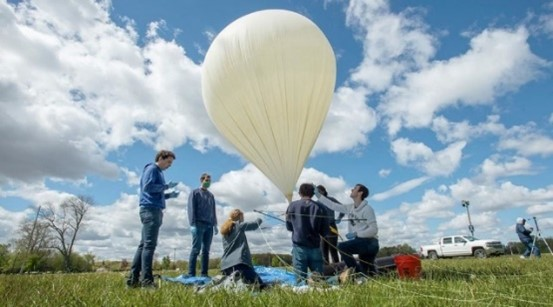
\includegraphics[width=.5\textwidth]{Pictures/HAB.jpg}
\caption{\emph{High Altitude Balloon}. Fuente: engineering.nd.edu }\label{fig:HAB}
\index{figures}
\end{figure}


\textbf{\emph{Zero-Pressure Balloons}:} Estos globos, con apertura en la parte inferior y conductos abiertos en los lados, permiten la liberación de gas y evitan el aumento de la presión interna a medida que se elevan. Sin embargo, su duración es limitada debido a la pérdida gradual de gas causada por el ciclo día/noche y las fluctuaciones de temperatura.

\begin{figure}[hbt!]
\centering
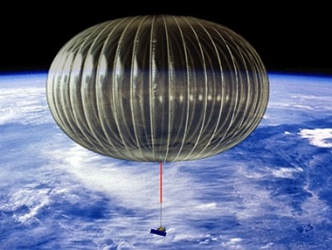
\includegraphics[width=.8\textwidth]{Pictures/ZeroP.png}
\caption{\emph{Zero-Pressure Balloon}. Fuente: https://stratocat.com.ar/ }\label{fig:ZeroP}
\index{figures}
\end{figure}

\textbf{\emph{Super-Pressure Balloons} (ULDB):} A diferencia de otros tipos de globos, en los ULDB el gas no puede escapar y la presión interna aumenta a medida que el gas se expande. Gracias a esta característica, la pérdida de gas en los globos de superpresión es mínima, lo que les permite volar durante períodos de tiempo más prolongados en comparación con los globos de presión cero.\\
Ambos tipos de globos no convencionales están hechos de polietileno, con un tamaño común de 40 millones de pies cúbicos. Se inflan con helio y pueden alcanzar una altitud de aproximadamente 120,000 pies, más del doble de la altitud de los aviones comerciales.


\begin{figure}[h!]
\centering
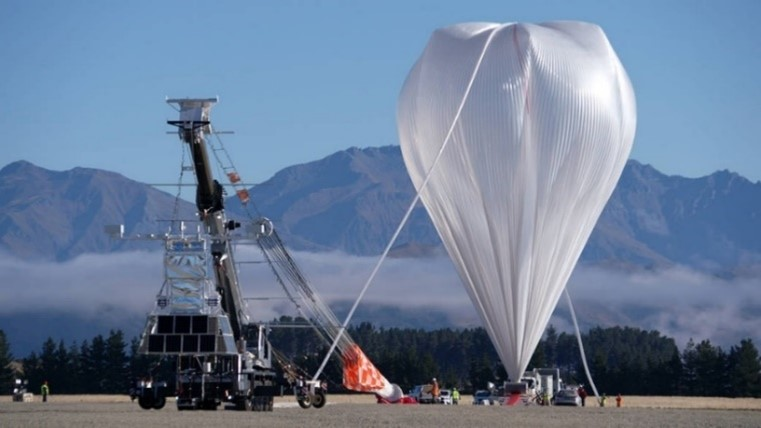
\includegraphics[width=.8\textwidth]{Pictures/SuperP.jpg}
\caption{\emph{Super-Pressure Balloon}. Fuente: nasa.gov }\label{fig:SuperP}
\index{figures}
\end{figure}

\newpage

Entre los logros más destacados se incluyen dos premios Nobel de Física, otorgados en 1936 y 2006, por el descubrimiento de los rayos cósmicos y el descubrimiento de la acelerada expansión del universo, respectivamente \cite{Nobel}.

\newpage


\section{Revisión del Estado del Arte de Sistemas de Eléctricos de Potencia (EPS) en aplicaciones de globos de gran altitud}

\vspace{0.5 cm}

Este trabajo se enfoca en el diseño y simulación de un sistema eléctrico de potencia (EPS) para misiones de corta duración con globos de gran altitud, priorizando la utilización de componentes electrónicos comerciales de bajo costo.

Al revisar la literatura, se observa la escasez de publicaciones directamente enfocadas en EPS para misiones con globos de gran altitud (HAB). Destacan trabajos, como el de la Universidad Sergio Arboleda en Colombia, que orienta el diseño de EPS para \emph{Balloonsats} y \emph{Cubesats} \cite{Vecino2013, comparasun,energiasat}, Estos trabajos se centran en modelos, simulación, experimentos y análisis exhaustivos de los componentes de un sistema de energía, abarcando celdas solares, baterías y convertidores DC-DC.


En las publicaciones, las aplicaciones de EPS están mayormente dirigidas a pequeños satélites, destacándose el estándar CubeSat. Proyectos del Kyushu Institute of Technology exhiben diseños que no solo cumplen con los requisitos de entrega de potencia, sino que también orientan el EPS hacia la recolección de datos, como voltaje, corriente y temperatura de baterías y paneles solares. El propósito es que esta información sea útil para comparativas de rendimiento y diagnóstico temprano de fallas \cite{jara2022orbit}. Asimismo, sobresale el proyecto Pycubed de la Universidad de Stanford, conocido por su programación totalmente en Python, su documentación y la utilización de componentes comerciales de bajo costo \cite{pycubed}.


Por otro lado, existen también diseños de EPS en aplicaciones híbridas de globos de gran altitud con CubeSat, como el proyecto TASEC-Lab de la Universidad Politécnica de Madrid. Este proyecto ejemplifica que los diseños con componentes comerciales para nanosatélites son aplicables para misiones de HAB, aplicándose de manera intercambiable. Además, el trabajo aborda factores ambientales relevantes para las misiones hacia la estratósfera, especialmente desde una perspectiva térmica en cada una de las capas previas. Se destaca una mención especial alrededor de los 11 km debido a una importante tasa de transferencia de calor por convección forzada. También se subraya la relevancia del control térmico pasivo con materiales como VDA, y se presentan pruebas ambientales en laboratorio, junto con un diseño simplificado de EPS que prioriza el funcionamiento y limita la complejidad innecesaria \cite{TASEC}.


Otros trabajos relevantes, aunque no centrados específicamente en EPS como un conjunto, abordan procesos relacionados. Destaca el trabajo de Eleazar Ramos en 2020, enfocado en la selección de baterías para nanosatélites según densidad energética, volumétrica y geometría \cite{Eleazar2020}. Revisiones exhaustivas sobre tecnología de baterías para misiones pequeñas, como la de Vaclav Knap en 2020, abordan criterios de selección, incluida la historia de vuelo y aplicaciones previas, junto con rigurosos procedimientos de pruebas para validar la seguridad de estas fuentes de almacenamiento de energía \cite{Knap2020}. Además, se encuentran estudios sobre el impacto térmico en el rendimiento de las baterías y la evolución con nuevos modelos, aspectos de alta relevancia para comprender las variables a controlar durante misiones en ambientes extremos \cite{Ma2018}.

En resumen, la revisión del estado del arte aporta modelos de arquitectura de EPS para aplicaciones desde vehículos eléctricos hasta nanosatélites, sin embargo, no se encuentran trabajos completos sobre el diseño de sistemas de energía para globos de gran altitud. Este vacío motiva el desarrollo de un EPS adaptado a las específicas condiciones de estas misiones para contribuir al avance de futuras investigaciones científicas que hagan uso de estas plataformas.

\newpage
\section{Metodología para el Diseño de Sistemas de Eléctricos de Potencia (EPS)}

\vspace{0.5 cm}

En relación a la metodología a implementar en este trabajo, la NASA ha establecido un ciclo de proyectos compuesto por siete fases, divididas en dos etapas fundamentales: formulación e implementación. La formulación abarca desde el estudio de conceptos hasta la completación tecnológica, mientras que la implementación se desarrolla desde el diseño final y fabricación hasta el cierre del proyecto, pasando por etapas cruciales como el ensamble, la integración y las pruebas \cite{NASA2016}. \\\\Además, el Modelo en V, ilustrado en la Fig. \ref{fig:fig_modelV}, ofrece una representación clara y coherente de esta metodología, aplicable específicamente al desarrollo de sistemas de energía para misiones de pequeños satélites \cite{IEEE_AESS_Distinguished_Lecture}. Dada la compatibilidad de este modelo con el enfoque de este trabajo, se considera prudente adoptarlo como una metodología con un historial probado en implementación.

\vspace{0.5 cm}

\begin{figure}[h]
  \centering
  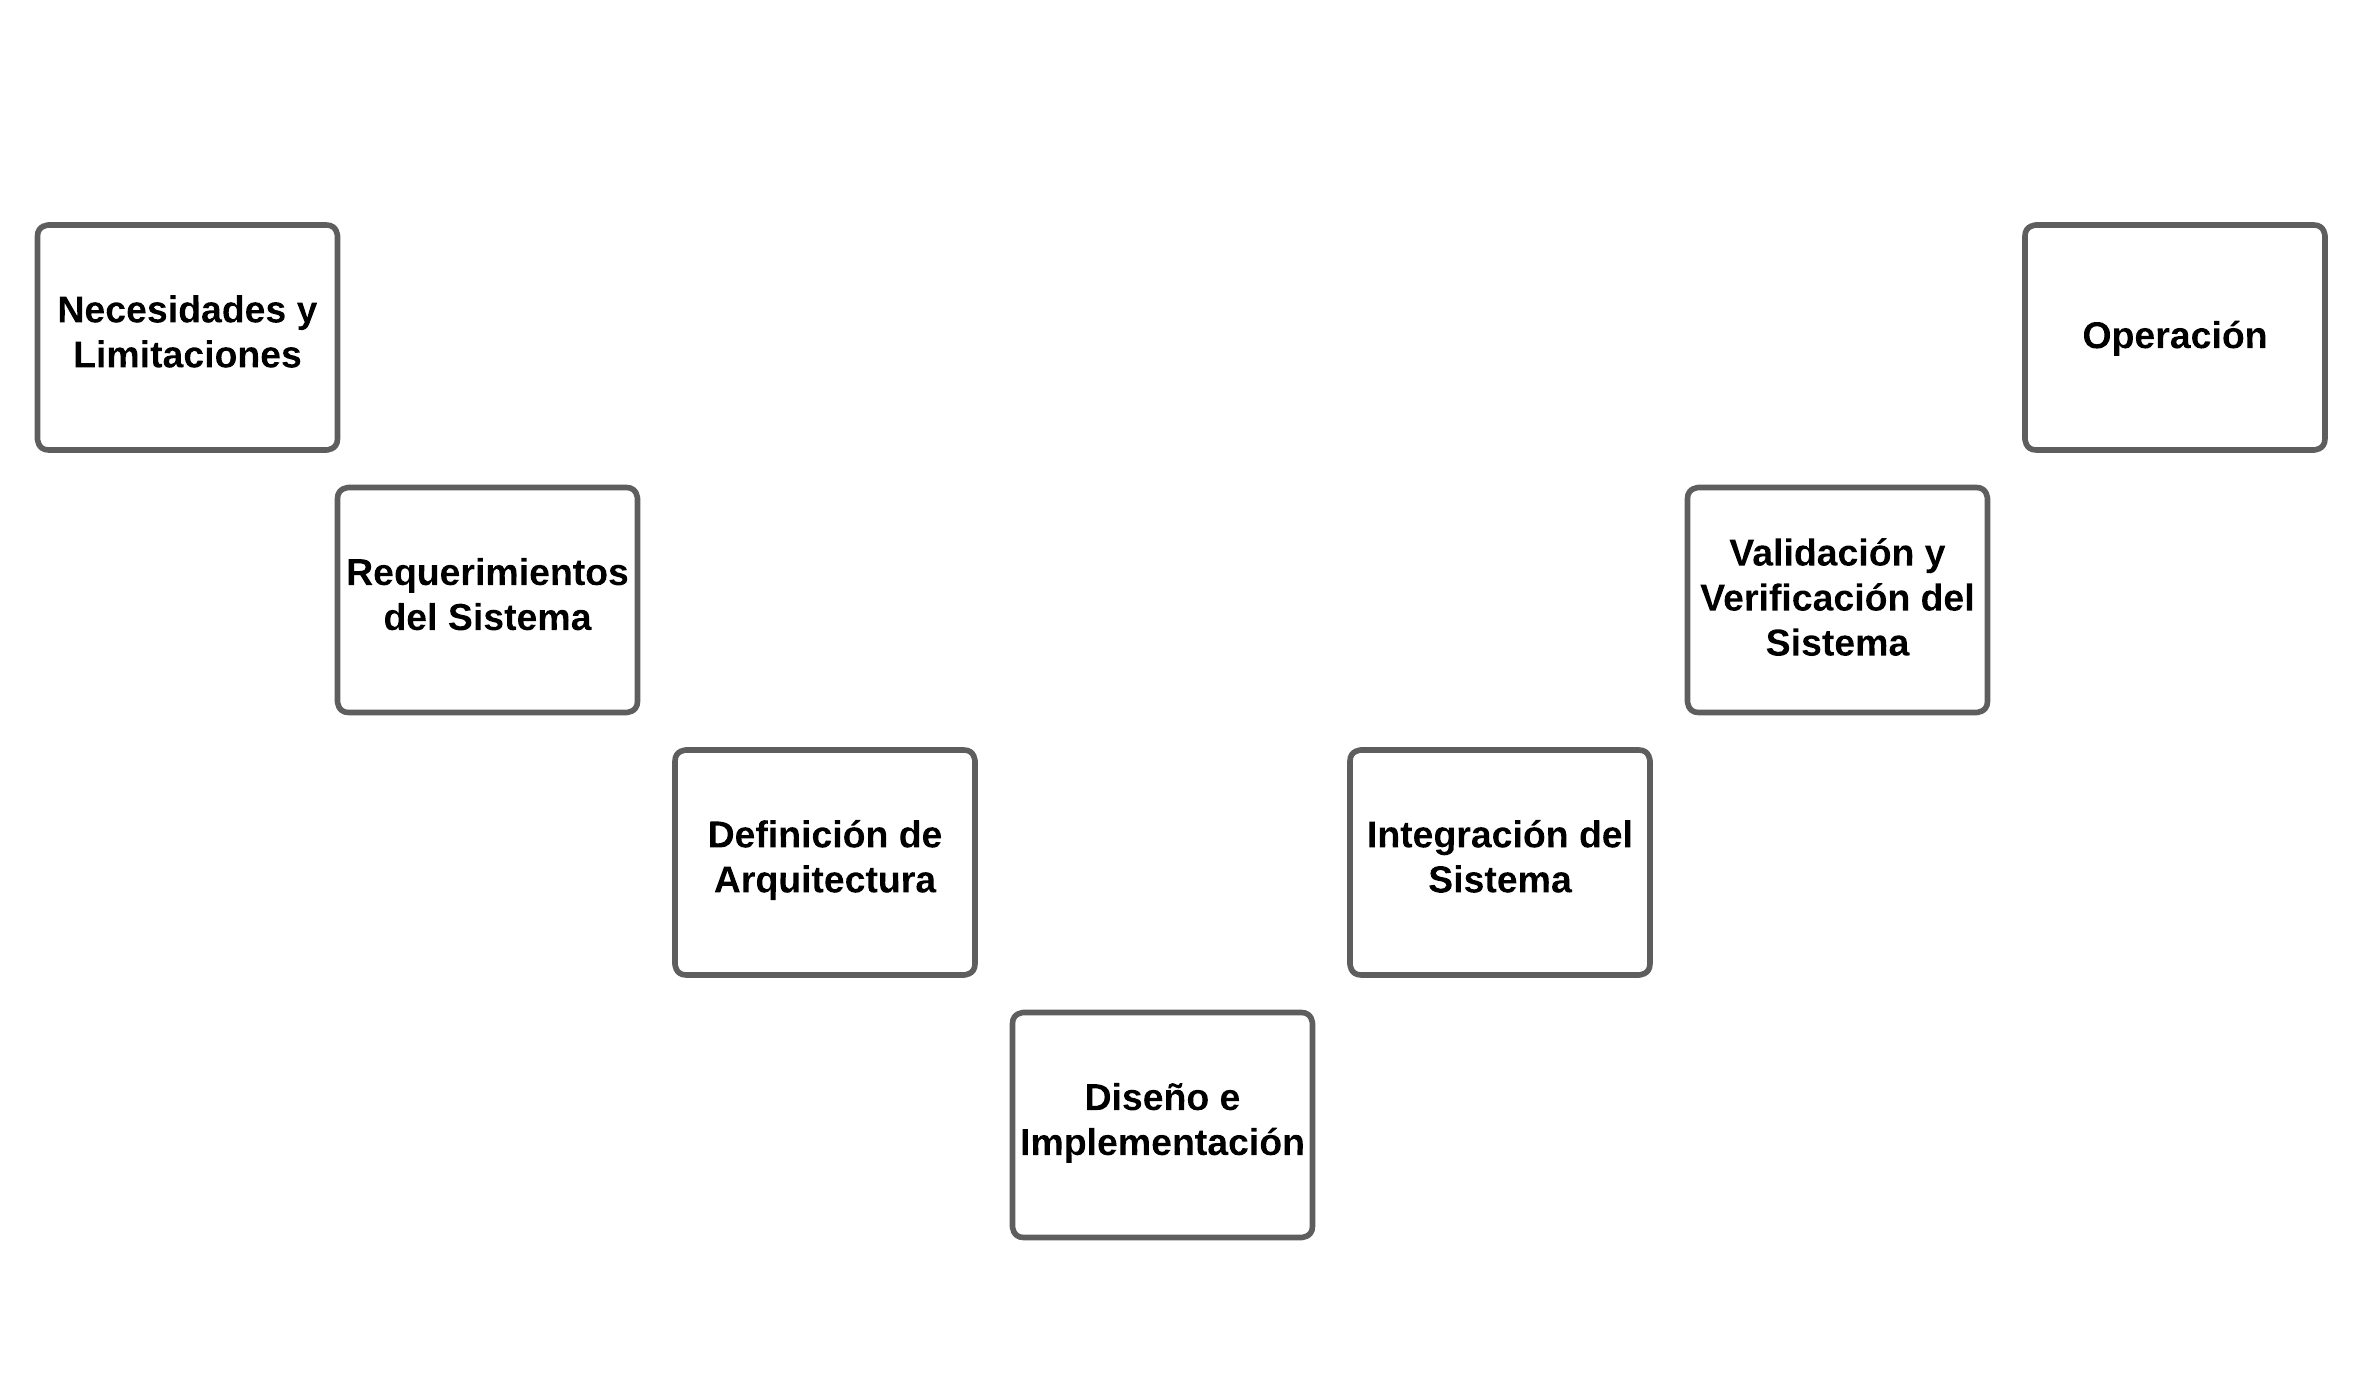
\includegraphics[width=\linewidth]{Pictures/ModeloV.png}
  \caption{Fases del modelo en V}
  \label{fig:fig_modelV}
\end{figure}


\subsection{Necesidades y Limitaciones}

En esta etapa, se busca caracterizar el sistema en función de su contexto de aplicación. Se identifican necesidades cruciales, como la resistencia a factores ambientales y la gestión eficiente del presupuesto energético. Además, se consideran las limitaciones específicas que el sistema debe abordar para adaptarse a las distintas condiciones de cada misión.

\subsection{Requerimientos del Sistema}

En esta fase, se concretizan las necesidades y limitaciones en una tabla de requerimientos. Es fundamental que estos estén claramente descritos, debidamente justificados y que cuenten con mecanismos de verificación medibles.

\subsection{Arquitectura}

Durante esta etapa, abordamos el diseño del sistema con un enfoque Top-Down, descomponiéndolo hasta alcanzar la mínima unidad funcional. Esto nos proporciona una comprensión detallada de la conexión y función conjunta de cada parte, sirviendo como base para las fases posteriores de integración. En esta fase, se detallan las entradas y salidas, tanto para el sistema en su vista más general como para cada una de sus subpartes.

\subsection{Diseño e Implementación}

En esta fase, transitamos del diseño funcional a la implementación física. Aquí, se realiza la selección de componentes en función de los requerimientos del sistema y de la arquitectura establecida. Se detallan las conexiones físicas a nivel de cada componente, definidas en el nivel más alto alcanzado en la arquitectura.

\subsection{Integración del Sistema}

La fase de integración comprende un proceso tanto a nivel de hardware como de software, con el objetivo de materializar el diseño funcional propuesto en la arquitectura.

\subsection{Validación y Verificación del Sistema}

En esta etapa, se define un plan de pruebas necesario para validar, a través de mediciones, que los requerimientos previamente establecidos se hayan alcanzado de manera efectiva.

\subsection{Operación}

Esta fase representa el punto culminante, donde el sistema integrado, validado y verificado, es puesto en funcionamiento en su entorno operativo.
 











\chapter{Necesidades y Limitaciones}
En este capítulo, se abordan las necesidades y limitaciones clave que deben considerarse al diseñar y simular un sistema de energía basado en componentes comerciales para globos de gran altitud en ambiente estratosférico. Estas consideraciones son fundamentales para asegurar un funcionamiento óptimo y eficiente del sistema en el desafiante entorno estratosférico. 

\hspace{1.27cm}Comenzaremos explorando las condiciones ambientales específicas a las que se enfrentará el sistema durante su operación en la estratosfera. Estas condiciones incluyen variaciones extremas de temperatura y presiones atmosféricas, entre otros factores, que plantean desafíos significativos en la selección y rendimiento de los componentes utilizados.

\hspace{1.27cm}Además, realizaremos un presupuesto energético del sistema para determinar la cantidad de energía requerida para alimentar el subsistema de telemetría, navegación y carga útil. Este análisis nos permitirá establecer los requisitos de potencia y energía que deben cumplirse, así como identificar oportunidades para optimizar la eficiencia energética y maximizar la autonomía del sistema.

\hspace{1.27cm}Asimismo, examinaremos las limitaciones de masa y volumen a las que el sistema está sujeto. Es esencial diseñar un sistema que cumpla con los requisitos establecidos según el contexto de aplicación, en este caso se evaluarán para la misión StratoBalloon.

\hspace{1.27cm}Adicionalmente, detallaremos de manera concisa las funciones del Sistema de Energía (EPS) y los protocolos de comunicación necesarios para la interconexión con los demás subsistemas de la sonda de HAB. Esto permitirá comprender de forma integral el papel del EPS en el funcionamiento global del sistema.

\hspace{1.27cm}Por último, obtendremos una tabla resumen que recopilará los requerimientos identificados en las secciones anteriores. Esta tabla ofrecerá una visión general y clara de las necesidades y limitaciones del sistema de energía propuesto, así como los mecanismos de verificación.



%REQUERIMIENTOS AMBIENTALES

\section{Condiciones ambientales}

La operación efectiva de un sistema de energía para globos de gran altitud en ambiente estratosférico es fundamental para garantizar el éxito de la misión. Este logro depende en gran medida de la comprensión y abordaje adecuado de las condiciones ambientales a las que estará expuesto.

La utilización de software de predicción de trayectoria es una herramienta esencial en misiones de \emph{High-Altitude Balloons }(HAB), ya que nos permite estimar la zona de aterrizaje, planificar la ruta de vuelo y definir el procedimiento de recuperación. Entre los programas más comúnmente utilizados para esta tarea se encuentran el \emph{Cambridge University Spaceflight} (CUSF) \cite{Cambridge}, \emph{Balloon Trajectory Forecasts} de la universidad de Wyoming \cite{uwyo_balloon_traj} y \emph{Balloon Prediction } \cite{noaa_wvap_sw}. Todos estos simuladores han sido desarrollados basados en el modelo \emph{Global Forecast System} (GFS) de la NOAA \cite{NOAA2023}.

De las alternativas disponibles, hemos decidido utilizar el simulador de la Universidad de Cambridge debido a que nos permite descargar directamente los datos en formato CSV y proporciona información detallada de localización con marcas de tiempo, que será de gran utilidad para nuestro análisis.


\begin{figure}[hbt!]
\centering
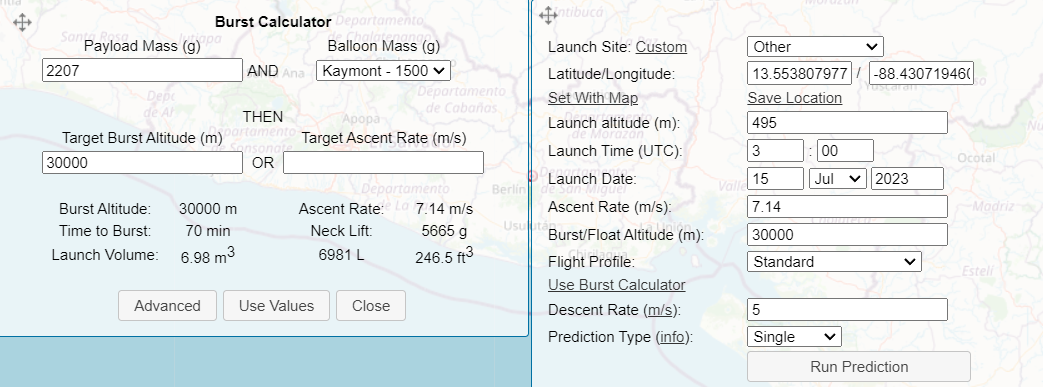
\includegraphics[width=0.75\textwidth]{Pictures/SimulacionParametros.png}
\caption{Valores de entrada para simulador de trayectoria CUSF }\label{fig:SimuladorParametros}
\index{figures}
\end{figure}

\begin{figure}[hbt!]
\centering
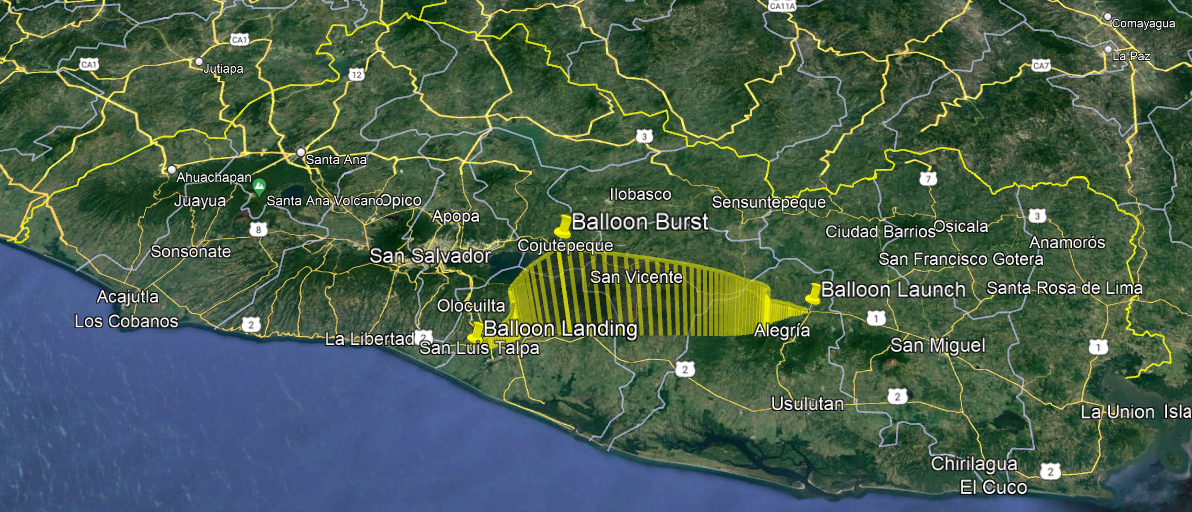
\includegraphics[width=0.75\textwidth]{Pictures/ruta.png}
\caption{Predicción realizada en CUSF visualizada en Google Earth }\label{fig:ruta}
\index{figures}
\end{figure}

Para mejorar nuestra comprensión del comportamiento de variables clave como temperatura y presión durante la misión, es fundamental incorporar el estándar atmosférico ISA en nuestro análisis. El software de CUSF nos ofrece datos de latitud, longitud y altitud, junto con marcas de tiempo con un muestreo cada minuto, lo que facilita la estimación de la duración total de la misión y las razones de cambio en primer y segundo orden para cada variable.

Esta potente combinación nos proporciona una perspectiva más clara y precisa del entorno atmosférico durante todo el vuelo, enriqueciendo significativamente nuestra comprensión de las condiciones ambientales y su evolución en la misión.



\begin{figure}[hbt!]
\centering
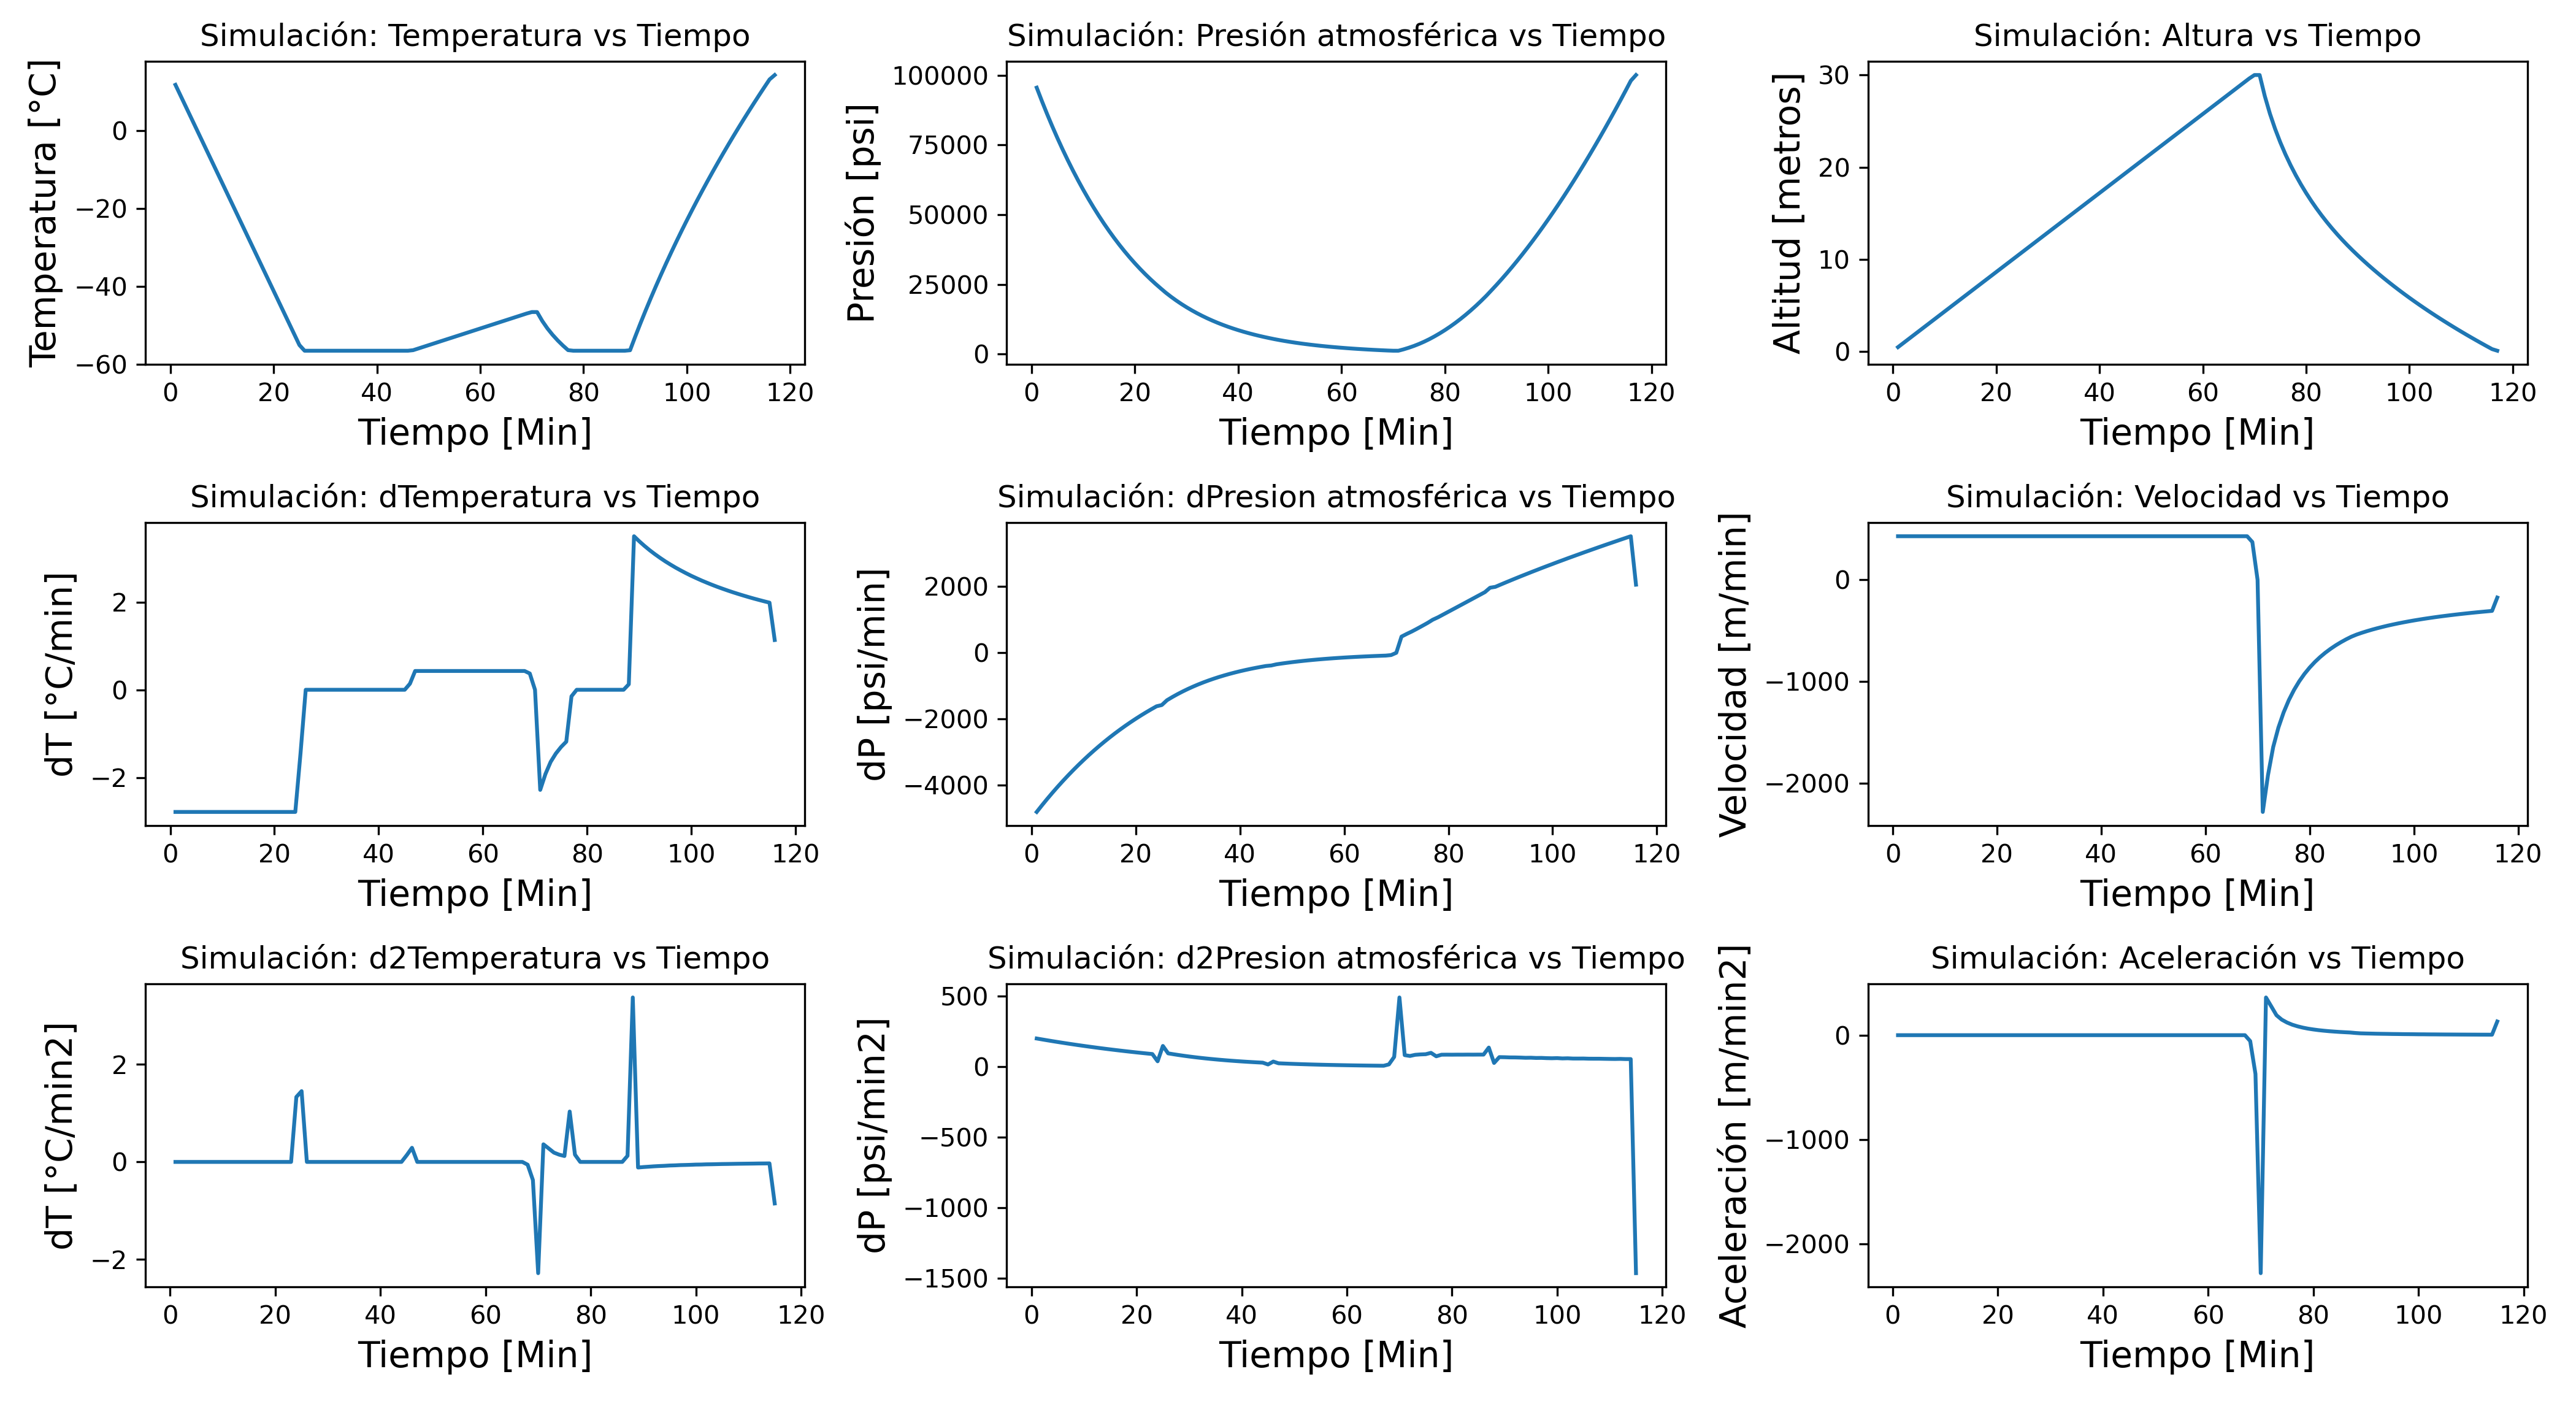
\includegraphics[width=1\textwidth]{Pictures/EnviromentalVariables.png}
\caption{Variables atmosféricas simuladas para una misión de HAB hacia 30 km.}\label{fig:Ambiente}
\index{figures}
\end{figure}

El desarrollo de cálculos en Python desarrollado en trabajos previos  \cite{stratoballoon_eps_batterytest} \cite{osmin-lab} muestra como resultado un comportamiento crítico (ver Fig.\ref{fig:Ambiente}). Las condiciones extremas en la estratósfera pueden alcanzar valores límites de -56.50\degree{}C y 1.20\% de la presión atmosférica estándar. En cuanto a las razones de cambio, se obtuvieron valores máximos de -2.78\degree{}C por minuto y una pérdida de presión atmosférica de 4.74\% por minuto.

Coincidiendo con otros estudios, como el experimento TASEC-Lab \cite{TASEC}, hemos identificado una franja crítica durante el ascenso, alrededor de la tropopausa a 11 km de altitud, con la mayor variación térmica. Este punto es crucial para la selección de componentes y la consideración de sistemas de control térmico.



% Requerimientos Energéticos
\section{Presupuesto energético}

En esta sección, desarrollaremos el presupuesto energético para determinar los requisitos de energía de la misión StratoBallon. La misión se divide en tres subsistemas: telemetría, navegación y carga útil (cámara RGB). Según simulaciones, se estima un tiempo de vuelo promedio de 2 horas para la sonda StratoBalloon. Sin embargo, por seguridad y proceso de recuperación, se añaden 4 horas adicionales, donde solo se requerirá la operación continua de navegación y telemetría.

El presupuesto energético, dividido por bus, se encuentra detallado en las Tablas \ref{tab:cuadro-cargas1} y \ref{tab:cuadro-cargas2}.\\



\begin{table}[!ht]
    \centering
    \renewcommand{\arraystretch}{1.2}
    \caption{Cuadro de cargas para bus 3.3v}
    \label{tab:cuadro-cargas1}
    \begin{tabularx}{1.1\textwidth}{llllllll}
    \hline
    \textbf{Descripción} & \textbf{Cantidad} & \textbf{Susbsistema} & \textbf{I [mA]} & \textbf{P [W]} & \textbf{t [h]} & \textbf{E [Wh]} & \textbf{Q [mAh]} \\
    \hline
    \text{MCU 1} & 1 unidad& Telemetría & 93.00 & 0.31 & 6.00 & 1.84 & 558 \\ 
    \text{LoRa} & 1 unidad & Telemetría & 630.00 & 2.08 & 6.00 & 12.47 & 3780 \\ 
    \text{MCU 2} & 1 unidad & Navegación & 61.00 & 0.20 & 6.00 & 1.21 & 366.00 \\ 
    \text{GNSS} & 1 unidad & Navegación & 100.00 & 0.33 & 6.00 & 1.98 & 600.00 \\ 
    \text{RTD} & 1 unidad & Navegación & 3.50 & 0.01 & 6.00 & 0.07 & 21.00 \\ 
    \text{IMU} & 1 unidad & Navegación & 0.60 & 0.00 & 6.00 & 0.01 & 3.60 \\ 
    \text{MCU 3} & 1 unidad & Carga útil & 70.00 & 0.23 & 2.00 & 0.46 & 140.00 \\ 
    \text{Cámara IR} & 1 unidad & Carga útil & 25.00 & 0.08 & 2.00 & 0.17 & 50.00 \\\hline 
    & & \textbf{I Máx.} & \text{983.10} & & & & \textbf{5518.6} \\ \hline
    \end{tabularx}
\end{table}

\begin{table}[!ht]
    \centering
    \renewcommand{\arraystretch}{1.2}
    \caption{Cuadro de cargas para bus 5.0v}
    \label{tab:cuadro-cargas2}
    \begin{tabularx}{1.1\textwidth}{llllllll}
        \hline
        \textbf{Descripción} & \textbf{Cantidad} & \textbf{Subsistema} & \textbf{I [mA]} & \textbf{P [W]} & \textbf{t [h]} & \textbf{E [Wh]} & \textbf{Q [mAh]} \\
        \hline
        RTC & 1 unidad & Navegación & 0.30 & 0.00 & 6.00 & 0.01 & 1.80 \\
        Buzzer & 1 unidad & Navegación & 24.00 & 0.12 & 6.00 & 0.72 & 144 \\
        Barómetro & 1 unidad & Navegación & 0.00 & 0.00 & 6.00 & 0.00 & 0.00 \\
        MUX & 1 unidad & Navegación & 100.00 & 0.50 & 6.00 & 3.00 & 600 \\
        Datalogger 1 & 1 unidad & Navegación& 6.00 & 0.03 & 6.00 & 0.18 & 36 \\
        Cámara & 1 unidad & Carga útil & 260.00 & 1.30 & 2.00 & 2.60 & 520 \\
        Datalogger 2 & 1 unidad & Carga útil & 12.00 & 0.06 & 2.00 & 0.12 & 24\\\hline
        ~ & ~ & \textbf{I Máx.} & \text{402.30} & ~ & ~ & ~ & \textbf{1325.8} \\
        \hline
    \end{tabularx}
\end{table}



% REQUERIMIENTOS DE MASA Y VOLUMEN

\section{Limitaciones de Masa y Volumen}

El diseño del EPS para la misión StratoBalloon se ve restringido por el contexto de la tesis y la fase avanzada de la misión. Las dimensiones y materiales de la estructura impresa ya han sido definidos \cite{barahona2022diseno}. Los componentes electrónicos de los otros subsistemas también han sido seleccionados, determinando el espacio disponible.

El módulo central (Fig. \ref{fig:imagen1}) reserva dos niveles inferiores estratégicamente ubicados para el EPS, separados por una distancia uniforme de 2.54 cm (Fig. \ref{fig:imagen2}), basada en las medidas detalladas en la Fig. \ref{fig:PlanoPCB}.

Es importante destacar que el peso máximo asignado al EPS en esta misión es de 600 gramos.



\begin{figure}[b]
  \centering
  \begin{subfigure}[b]{0.35\textwidth}
    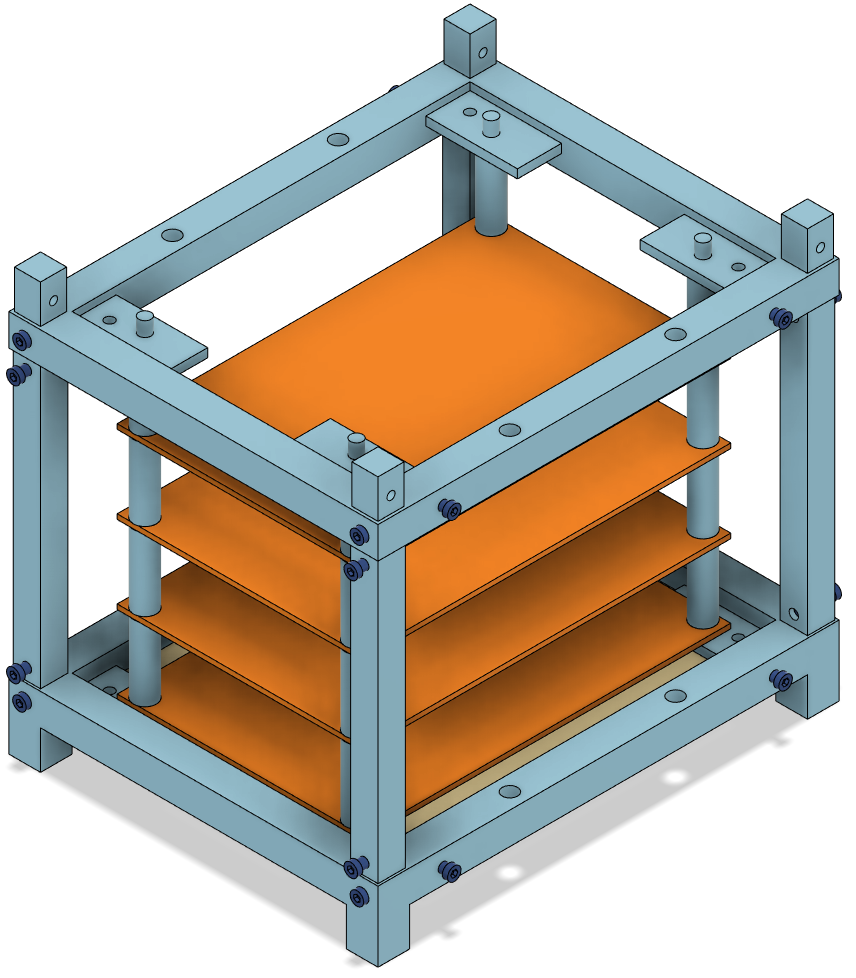
\includegraphics[width=\textwidth]{Pictures/3DPrinting.png}
    \caption{Vista 1}
    \label{fig:imagen1}
  \end{subfigure}
  \hfill
  \begin{subfigure}[b]{0.40\textwidth}
    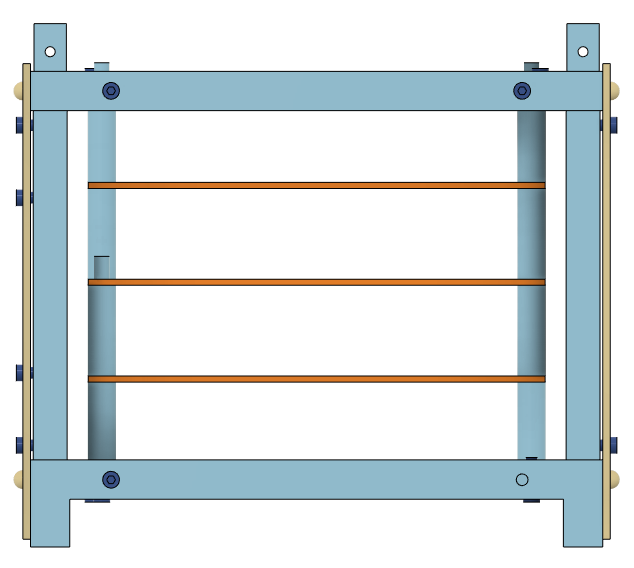
\includegraphics[width=\textwidth]{Pictures/Lateral3DPrinting.png}
    \caption{Vista 2}
    \label{fig:imagen2}
  \end{subfigure}

  \caption{Estructura de impresión 3D}
  \label{fig:dos_imagenes}
\end{figure}
\begin{figure}[hbt!]
\centering
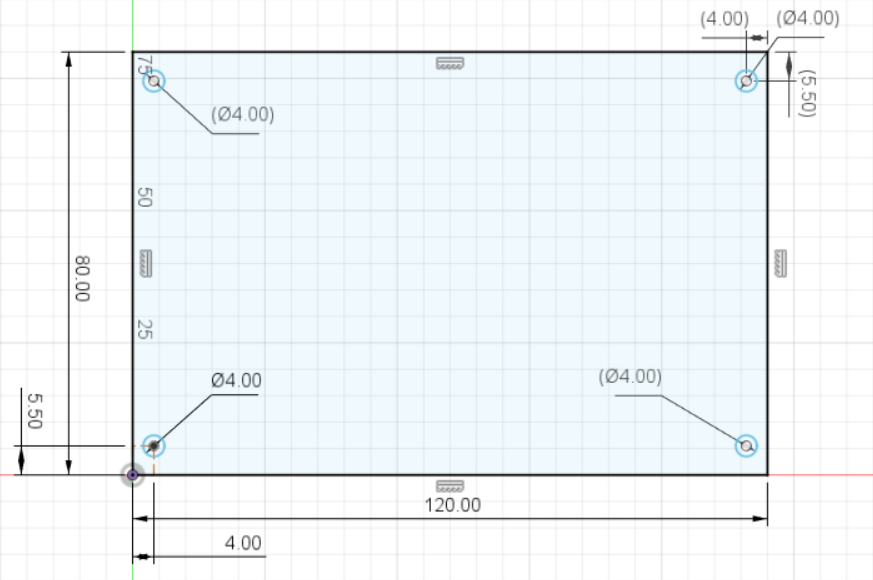
\includegraphics[width=0.75\textwidth]{Pictures/PlanoC.png}
\caption{Dimensiones de PCB en [mm]}\label{fig:PlanoPCB}
\index{figures}
\end{figure}

% RESUMEN DE REQUERIMIENTOS
\section{Resumen de requerimientos}
\vspace{0.5 cm}

El EPS cumple sus funciones principales durante la misión y permite la adquisición de datos para análisis posteriores. A continuación, se detallan los requerimientos del EPS en la Tabla \ref{tab:requerimientos-eps}.

\begin{table}[!ht]
    \centering
    \renewcommand{\arraystretch}{1.2}
    \caption{Requerimientos del EPS}
    \label{tab:requerimientos-eps}
    \begin{tabular}{l|p{4.8cm}|p{4.8cm}|p{4.8cm}}
    \hline
    \textbf{ID} & \textbf{Descripción} & \textbf{Justificación} & \textbf{Mecanismo de verificación} \\
    \hline
    R1 & Resistencia al vacío térmico, temperatura mínima de hasta -56.50°C y 1.20\% de presión atmosférica.& Resultados en simulaciones. & Ensayos en cámara de vacío térmico (Ver a detalle en Anexo \ref{ap:vaciotermico})
 \\
    \hline
    R2 & El EPS debe proveer una línea de alimentación de 3.3 V $\pm$ 1\% con una corriente mínima de 983.1 mA $\pm$ 1\%. & Bus de alimentación. & Medición de V y I.\\
    \hline
    R3 & El EPS debe proveer una línea de alimentación de 5.0 V $\pm$ 1\% con una corriente mínima de 402.30 mA $\pm$ 1\% & Bus de alimentación. & Medición de V y I. \\
    \hline
    R4 & No debe exceder una masa de 600 g. & Limitación de masa. & Medición de masa. \\
    \hline
    R5 & 2 PCB de 12x8 cm con 2.5 cm de altura.  & Limitación de espacio. & Medición de longitud.\\
    \hline
    R6 & Registro de V \text{[v]} y I \text{[mA]}. & Función deseable. & Ensayo de registro de datos. \\
    \hline
    R7 & Registro de T [\text{\textdegree{}C}] y P\text{ [atm]}.  & Función deseable. & Ensayo de registro de datos. \\
    \hline
    R8 & Comunicación I2C. Recepción desde Navegación de la señal de control ON/OFF de carga útil. Transmisión de SoC a telemetría.& Integración de subsistemas. & Ensayo de comunicación. \\
    \hline
    R9 & Control ON-OFF: carga útil.& Ahorro de energía. & Ensayo de control ON-OFF. \\
    \hline
    R10 & Interruptor RBF (Remove before flight, retirar antes del vuelo) para encendido y apagado del EPS.& Seguridad de la Misión, útil para prevenir accidentes. & Medición de continuidad. \\\hline
    R11 & Cargador de baterías con fuente de alimentación VDC externa & Carga del banco de baterías & Medición de voltaje. \\
    \hline
    \end{tabular}
\end{table}






\chapter{Definición de Arquitectura}

En este capítulo, después de haber definido los requerimientos (Tabla \ref{tab:requerimientos-eps}), nos adentramos en la fase de diseño del sistema. La creación de una representación clara y significativa del sistema es de suma importancia en este proceso. Para lograrlo, debemos considerar dos enfoques fundamentales ampliamente utilizados en el campo de la ingeniería: el enfoque \emph{bottom-up} (de abajo hacia arriba) y el enfoque \emph{top-down} (de arriba hacia abajo) \cite{ford2008design}.

\hspace{1.27cm}En el enfoque \emph{bottom-up}, comenzamos con componentes básicos que se ensamblan gradualmente para formar el sistema completo. Podemos pensar en esto como la construcción de un automóvil a partir de neumáticos, motor, chasis y otros elementos fundamentales. Este enfoque nos insta a prestar atención a los detalles mientras construimos el sistema, manteniendo la simplicidad sin caer en niveles excesivos de profundidad.

\hspace{1.27cm}Por otro lado, el enfoque \emph{top-down} nos invita a partir de una visión general del sistema final. Dividimos este sistema en partes y subsistemas que trabajan en conjunto para alcanzar el objetivo general. Este método nos permite mantener una perspectiva amplia y clara, definiendo primero los componentes principales antes de adentrarnos en los detalles más finos.

\hspace{1.27cm}Al aplicar estos enfoques, debemos recordar que nuestro objetivo es definir un nivel base de funcionalidad. No debemos caer en la trampa de una profundización excesiva que podría llevar a complicaciones innecesarias. 

\hspace{1.27cm}En nuestro proceso de diseño, además, evaluamos modelos previos y valoramos factores de innovación y escalabilidad. Esta estrategia nos habilita para edificar sobre conocimientos previos y estar preparados para futuras mejoras en el sistema. Para los propósitos de esta tesis, hemos optado por implementar el enfoque \emph{Top-Down} utilizando diagramas y tablas que muestran las entradas y salidas par cada bloque funcional según los niveles de profundidad.
\newpage


%Decomposición funcional: Nivel 0

\section{Nivel 0}

\begin{figure}[h!]
\centering
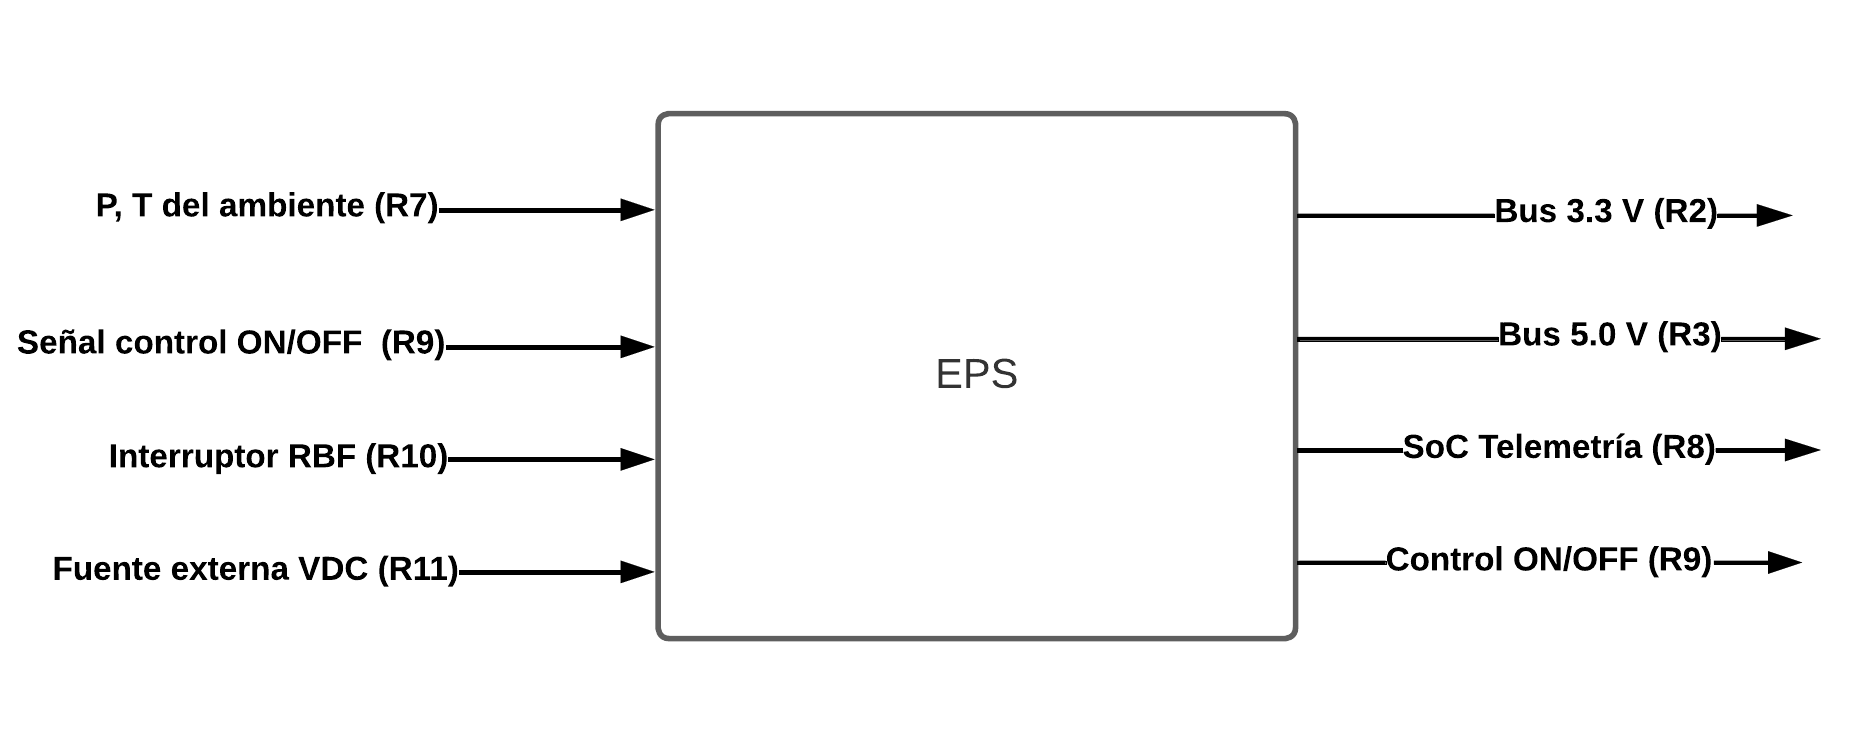
\includegraphics[width=\textwidth]{Pictures/Level0.png}
\caption{Diagrama funcional Nivel 0.}\label{fig:Level0}
\index{figures}
\end{figure}

\begin{table}[h]
    \centering
    \caption{Detalles de Nivel 0}
    \label{tab:nivel0}
    \begin{tabular}{ll}
    \toprule
        Módulo  & Electrical Power System (EPS) \\ 
    \midrule
        Entradas & 
        \begin{minipage}[t]{0.75\linewidth}
        - Presión atmosférica y temperatura ambiente. \\
        - Señales de navegación para control ON/OFF de carga útil. \\
        - Señal de interruptor RBF (Remove before flight).\\
        - Fuente externa VDC para el cargador de baterías.
        \end{minipage} \\
    \midrule
        Salidas & 
        \begin{minipage}[t]{0.75\linewidth}
        - Bus 3.3 V $\pm$ 1\%, 1.5A (factor de seguridad 1.25) \\
        - Bus 5.0 V $\pm$ 1\%, 0.6A factor de seguridad 1.25)\\
        - Estado de carga de baterías (SoC) \\
        - Control ON/OFF para carga útil, 5V $\pm$ 1\%
        \end{minipage} \\
    \midrule
        Funcionamiento & 
        \begin{minipage}[t]{0.75\linewidth}
El sistema se activa mediante un interruptor RBF y se alimenta con baterías de iones de litio 18650 recargadas por una fuente externa de VDC. Recopila datos de voltaje, corriente, presión atmosférica y temperatura ambiental, y proporciona dos buses de alimentación a 3.3 V y 5.0 V. Además, transmite el estado de carga de las baterías (SoC) al subsistema de telemetría y suministra energía a la carga útil bajo el control del subsistema de navegación.

        \end{minipage} \\
    \bottomrule
    \end{tabular}
\end{table}

\newpage

%Decomposición funcional: Nivel 1
%-**************************************

\section{Nivel 1}

\begin{figure}[h!]
\centering
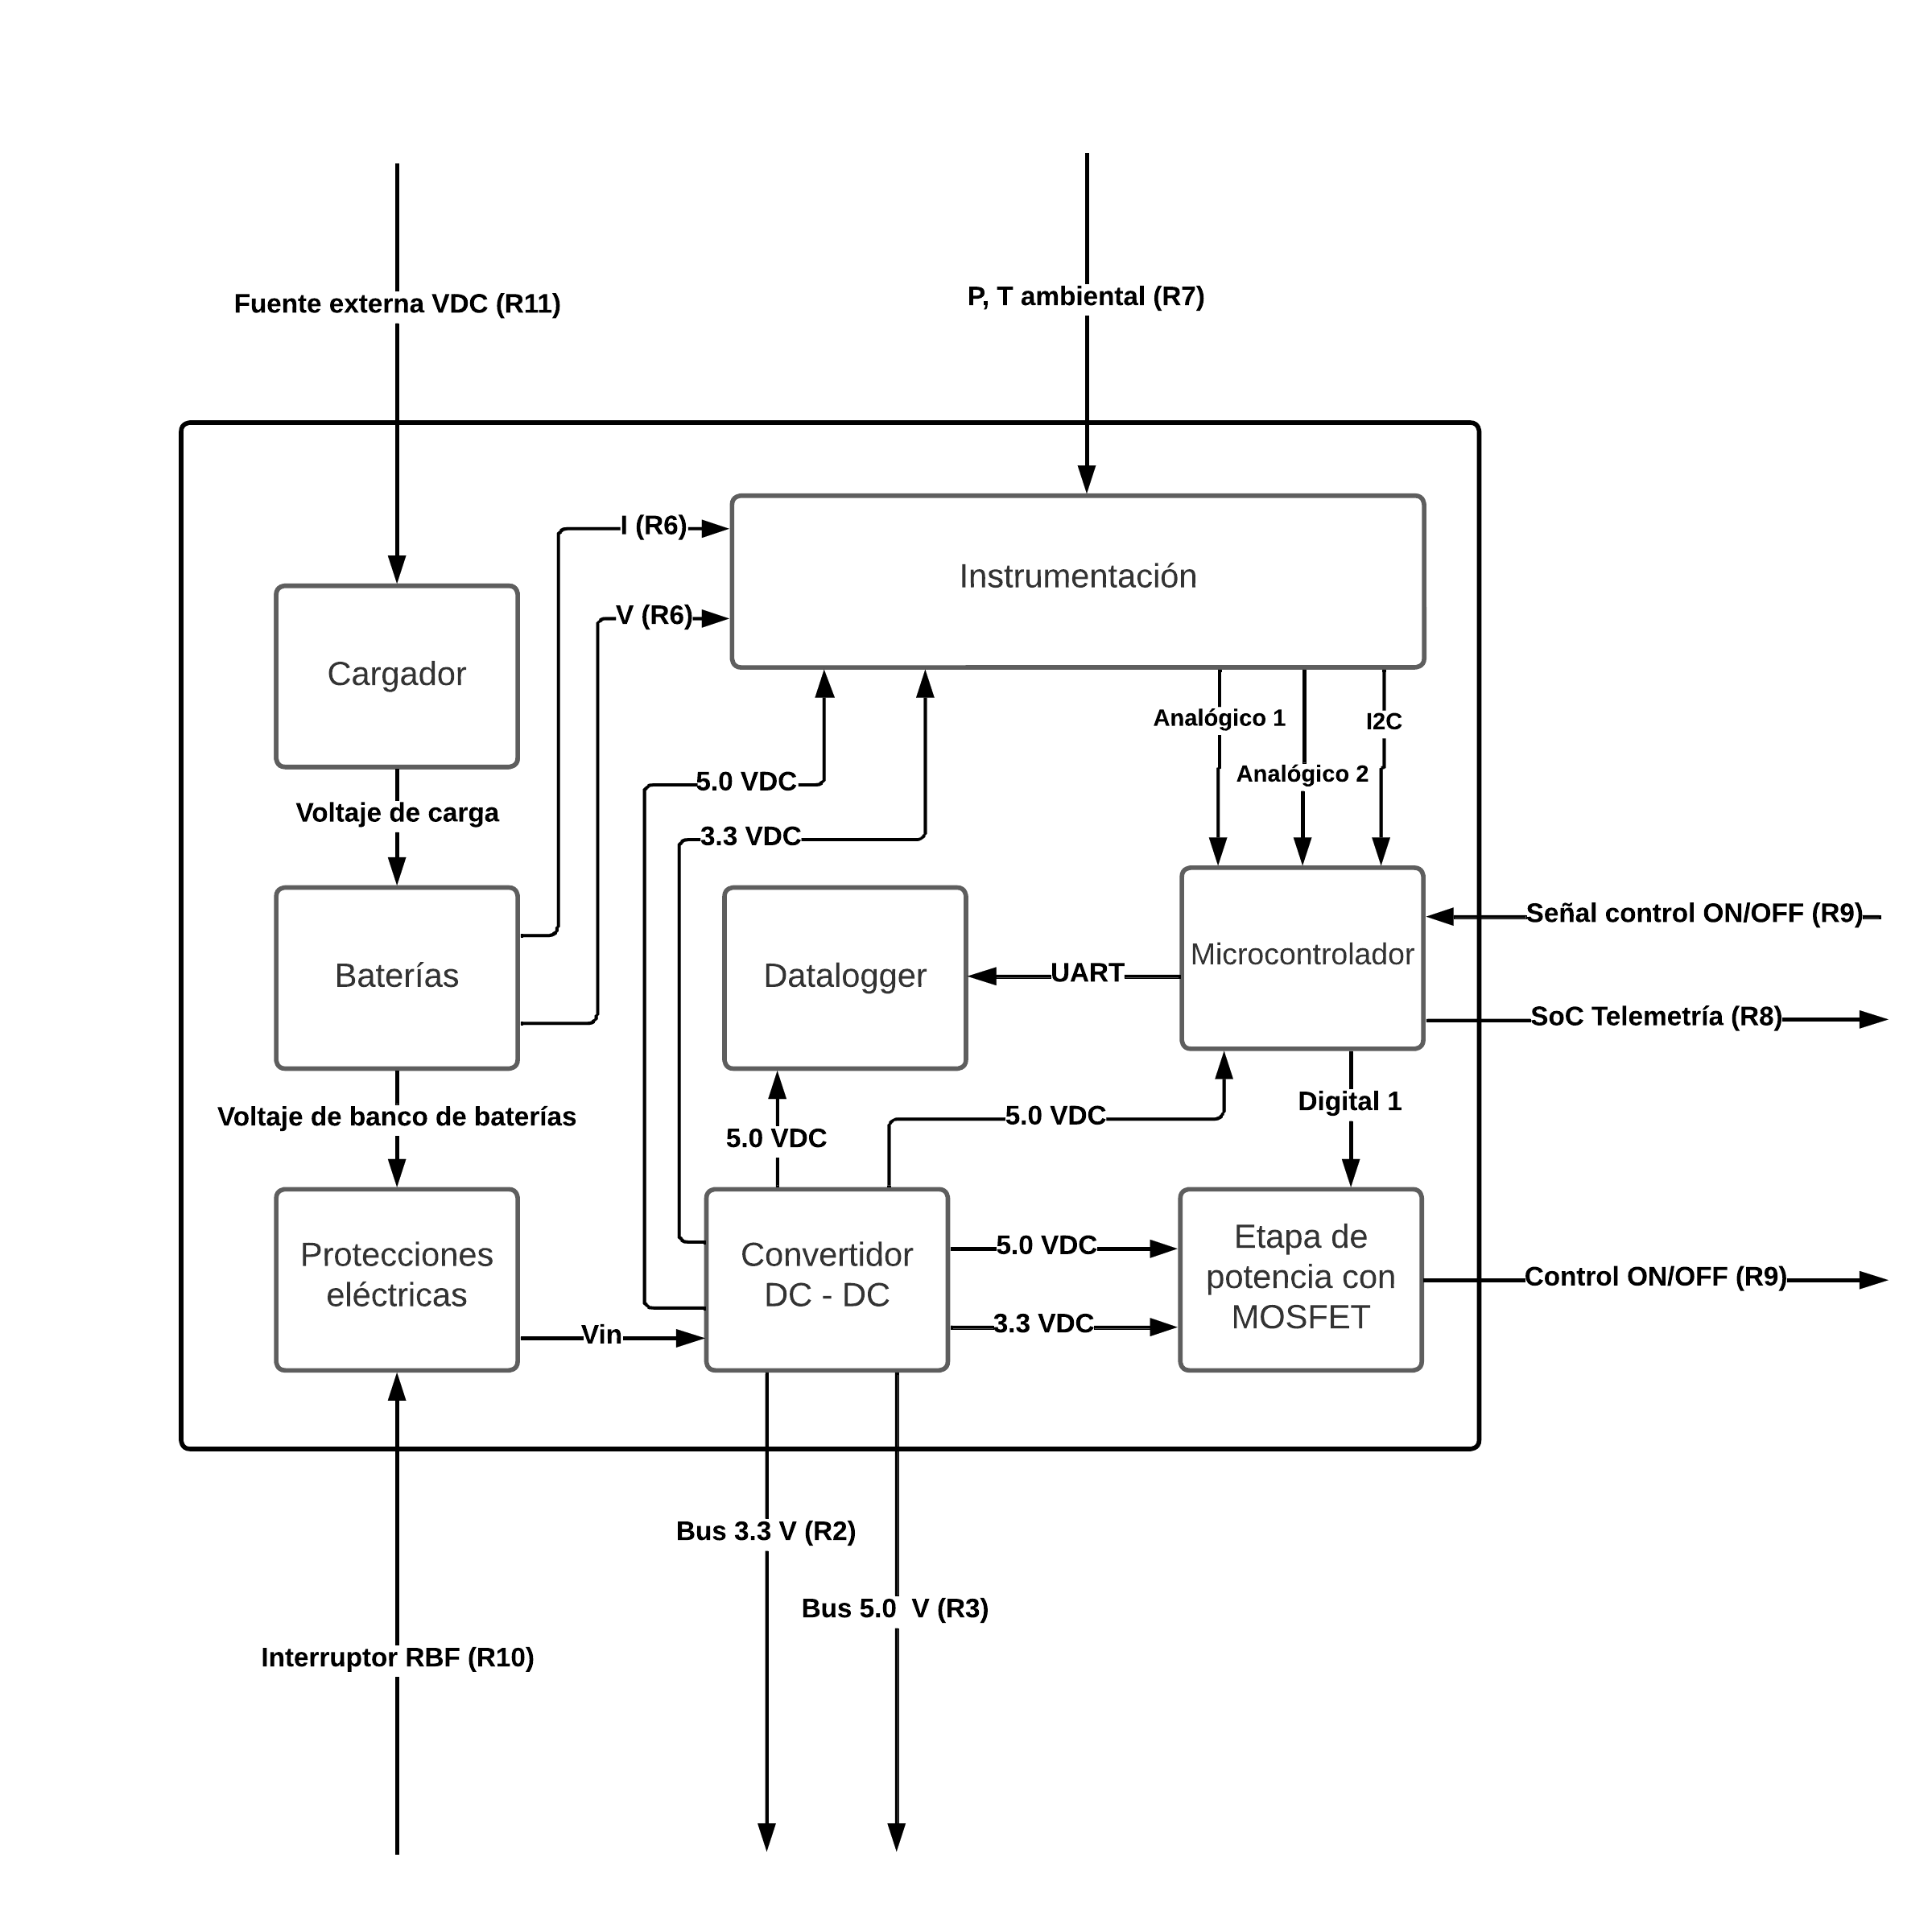
\includegraphics[width=0.8\textwidth]{Pictures/Level1.png}
\caption{Diagrama funcional Nivel 1.}\label{fig:Level1}
\index{figures}
\end{figure}

\begin{table}[h!]
    \centering
    \caption{Detalles de Nivel 1, cargador.}
    \label{tab:nivel1_cargador}
    \begin{tabular}{ll}
    \toprule
        Módulo  & Cargador\\ 
    \midrule
        Entradas & 
        \begin{minipage}[t]{0.75\linewidth}
 - Fuente externa VDC 5.0 V $\pm$ 1\% 
        \end{minipage} \\
    \midrule
        Salidas & 
        \begin{minipage}[t]{0.75\linewidth}
        - Voltaje de carga (4.2 v $\pm$ 1\%) para baterías Li-ion 18650.
        \end{minipage} \\
    \midrule
        Funcionamiento & 
        \begin{minipage}[t]{0.75\linewidth}
El cargador recibe energía de una fuente externa de tensión constante (\textit{VDC}). Su función principal es proporcionar una salida de $4.2 \, \text{V} \pm 1\%$ para cargar baterías de ion de litio 18650.

        \end{minipage} \\
    \bottomrule
    \end{tabular}
\end{table}
\newpage

%-**************************************
% BATERÍAS 
\begin{table}[!ht]
    \centering
    \caption{Detalles de Nivel 1, baterías.}
    \label{tab:nivel1_baterias}
    \begin{tabular}{ll}
    \toprule
        Módulo  & Baterías\\ 
    \midrule
        Entradas & 
        \begin{minipage}[t]{0.75\linewidth}
 - Voltaje de carga a $4.2 \, \text{V} \pm 1\%$ 
        \end{minipage} \\
    \midrule
        Salidas & 
        \begin{minipage}[t]{0.75\linewidth}
- El voltaje de salida del banco de baterías se determina mediante una configuración serie-paralelo de pilas con un voltaje nominal de 3.6 V.

        \end{minipage} \\
    \midrule
        Funcionamiento & 
        \begin{minipage}[t]{0.75\linewidth}
El banco de baterías tiene la función de entregar la potencia eléctrica requerida por el EPS.

        \end{minipage} \\
    \bottomrule
    \end{tabular}
\end{table}


%-**************************************

% PROTECCIONES ELÉCTRICAS

\begin{table}[h!]
    \centering
    \caption{Detalles de Nivel 1, protecciones eléctricas.}
    \label{tab:nivel1_protecciones}
    \begin{tabular}{ll}
    \toprule
        Módulo  & Protecciones Eléctricas\\ 
    \midrule
        Entradas & 
        \begin{minipage}[t]{0.75\linewidth}
 - Voltaje del banco de baterías.\\ - Señal de activación de interruptor RBF.
 
        \end{minipage} \\
    \midrule
        Salidas & 
        \begin{minipage}[t]{0.75\linewidth}
- Voltaje de entrada para etapa de regulación de voltaje.

        \end{minipage} \\
    \midrule
        Funcionamiento & 
        \begin{minipage}[t]{0.75\linewidth}
Consta de una protección tipo "Remove before Flight" y un interruptor de 4 polos para la desconexión de las pilas 18650.

        \end{minipage} \\
    \bottomrule
    \end{tabular}
\end{table}
%-**************************************

% REGULACIÓN DE VOLTAJE
\begin{table}[h!]
    \centering
    \caption{Detalles de Nivel 1, Convertidor DC-DC.}
    \label{tab:nivel1_protecciones}
    \begin{tabular}{ll}
    \toprule
        Módulo  & Convertidor DC-DC\\ 
    \midrule
        Entradas & 
        \begin{minipage}[t]{0.75\linewidth}
 - Voltaje del banco de baterías.
 
        \end{minipage} \\
    \midrule
        Salidas & 
        \begin{minipage}[t]{0.75\linewidth}
- Bus 3.3 V $\pm$ 1\%, 1.5A (factor de seguridad 1.25) \\
        - Bus 5.0 V $\pm$ 1\%, 0.6A factor de seguridad 1.25)\\

        \end{minipage} \\
    \midrule
        Funcionamiento & 
        \begin{minipage}[t]{0.75\linewidth}
La etapa de convertidores DC-DC transforma el voltaje de las pilas Li-ion 18650 del banco de baterías en dos buses de salida: uno de $5.0 \, \text{V} \pm 1\%$ que suministra al menos 983 mA y otro de $3.3 \, \text{V} \pm 1\%$ con una capacidad mínima de 402.30 mA. Estos buses alimentan los subsistemas electrónicos y las cargas del sistema.


        \end{minipage} \\
    \bottomrule
    \end{tabular}
\end{table}

%-**************************************

% ETAPA DE POTENCIA MOSFET

\begin{table}[h!]
    \centering
    \caption{Detalles de Nivel 1, etapa de potencia con MOSFET.}
    \label{tab:nivel1_MOSFET}
    \begin{tabular}{ll}
    \toprule
        Módulo  & Etapa de potencia con MOSFET\\ 
    \midrule
        Entradas & 
        \begin{minipage}[t]{0.75\linewidth}
 - Alimentación $5.0 \, \text{V} \pm 1\%$\\
 - Alimentación $3.3 \, \text{V} \pm 1\%$\\
 - Señal digital de activación de microcontrolador (Digital 1)
 
        \end{minipage} \\
    \midrule
        Salidas & 
        \begin{minipage}[t]{0.75\linewidth}
    - Control de activación ON/OFF a tensión $5.0 \, \text{V} \pm 1\%$

        \end{minipage} \\
    \midrule
        Funcionamiento & 
        \begin{minipage}[t]{0.75\linewidth}
Activa o desactiva la fuente de alimentación de la caerga útil. 

        \end{minipage} \\
    \bottomrule
    \end{tabular}
\end{table}

\vspace{4 cm}
%****************************************
% Microcontrolador

\begin{table}[h!]
    \centering
    \caption{Detalles de Nivel 1, microcontrolador.}
    \label{tab:nivel1_Microcontrolador}
    \begin{tabular}{ll}
    \toprule
        Módulo  & Microcontrolador\\ 
    \midrule
        Entradas & 
        \begin{minipage}[t]{0.75\linewidth}
 - Alimentación $5.0 \, \text{V} \pm 1\%$\\
 - Señal de activación para control ON/OFF proveniente de subsistema de Navegación vía I2C.\\
- Señal analógica 1 de etapa de instrumentación.\\
- Señal analógica 2 de etapa de instrumentación.\\
- Comunicación I2C de etapa de instrumentación.\\
 
        \end{minipage} \\
    \midrule
        Salidas & 
        \begin{minipage}[t]{0.75\linewidth}
    - Comunicación UART con Datalogger.\\
    - Señal digital de activación de microcontrolador (Digital 1)\\
    - Estado de carga (SoC) para subsistema de Telemetría vía I2C.

        \end{minipage} \\
    \midrule
        Funcionamiento & 
        \begin{minipage}[t]{0.75\linewidth}
El microcontrolador se alimenta con una tensión de $5.0 \, \text{V} \pm 1\%$. Recibe lecturas analógicas (1 y 2) de la etapa de instrumentación, así como datos a través de la comunicación I2C. Además, recibe una señal digital del subsistema de Navegación, la cual está asociada a un control ON/OFF para la activación de la carga útil.

En lo que respecta a las salidas, envía datos de registro al Datalogger a través de una conexión UART. Utiliza el pin Digital 1 para activar o desactivar la etapa de potencia que alimenta la carga útil. Finalmente, después de un procesamiento interno, el microcontrolador calcula y transmite vía I2C el estado de carga (SoC) al subsistema de telemetría.


        \end{minipage} \\
    \bottomrule
    \end{tabular}
\end{table}

%***************************************
% Datalogger
% Microcontrolador

\begin{table}[h!]
    \centering
    \caption{Detalles de Nivel 1, Datalogger.}
    \label{tab:nivel1_Datalogger}
    \begin{tabular}{ll}
    \toprule
        Módulo  & Datalogger\\ 
    \midrule
        Entradas & 
        \begin{minipage}[t]{0.75\linewidth}
 - Alimentación $5.0 \, \text{V} \pm 1\%$\\
 - Recepción de datos vía UART, provenientes del Microcontrolador.
 
        \end{minipage} \\
    \midrule
        Salidas & 
        \begin{minipage}[t]{0.75\linewidth}
    - Registro de datos en MicroSD

        \end{minipage} \\
    \midrule
        Funcionamiento & 
        \begin{minipage}[t]{0.75\linewidth}
El datalogger alimentado a  $5.0 \, \text{V} \pm 1\%$ recibe datos vía UART y los registra en una MicroSD.

        \end{minipage} \\
    \bottomrule
    \end{tabular}
\end{table}
% ESPACIADO VERTICAL
\vspace{4 cm}
%***************************************
% INSTRUMENTACIÓN

\begin{table}[h!]
    \centering
    \caption{Detalles de Nivel 1, Instrumentación.}
    \label{tab:nivel1_Instrumentacion}
    \begin{tabular}{ll}
    \toprule
        Módulo  & Instrumentación\\ 
    \midrule
        Entradas & 
        \begin{minipage}[t]{0.75\linewidth}
  - Alimentación $5.0 \, \text{V} \pm 1\%$\\
   - Alimentación $3.3 \, \text{V} \pm 1\%$\\
 - Presión atmosférica y emperatura ambiente.
 
        \end{minipage} \\
    \midrule
        Salidas & 
        \begin{minipage}[t]{0.75\linewidth}
    - Señal analógica 1\\
    - Señal analógica 2 \\
    - Señal vía I2C

        \end{minipage} \\
    \midrule
        Funcionamiento & 
        \begin{minipage}[t]{0.75\linewidth}
La etapa de instrumentación se alimenta con $5.0 \, \text{V} \pm 1\%$ y $3.3 \, \text{V} \pm 1\%$, y recibe señales analógicas del entorno, como temperatura y presión. Luego, traduce esta información ambiental en señales digitales, así también las medición eléctricas dentro del mismo EPS como el voltaje y corriente del banco de baterías.

        \end{minipage} \\
    \bottomrule
    \end{tabular}
\end{table}


% Nueva página para Nivel 2
\newpage

\section{Nivel 2}

\begin{figure}[h!]
\centering
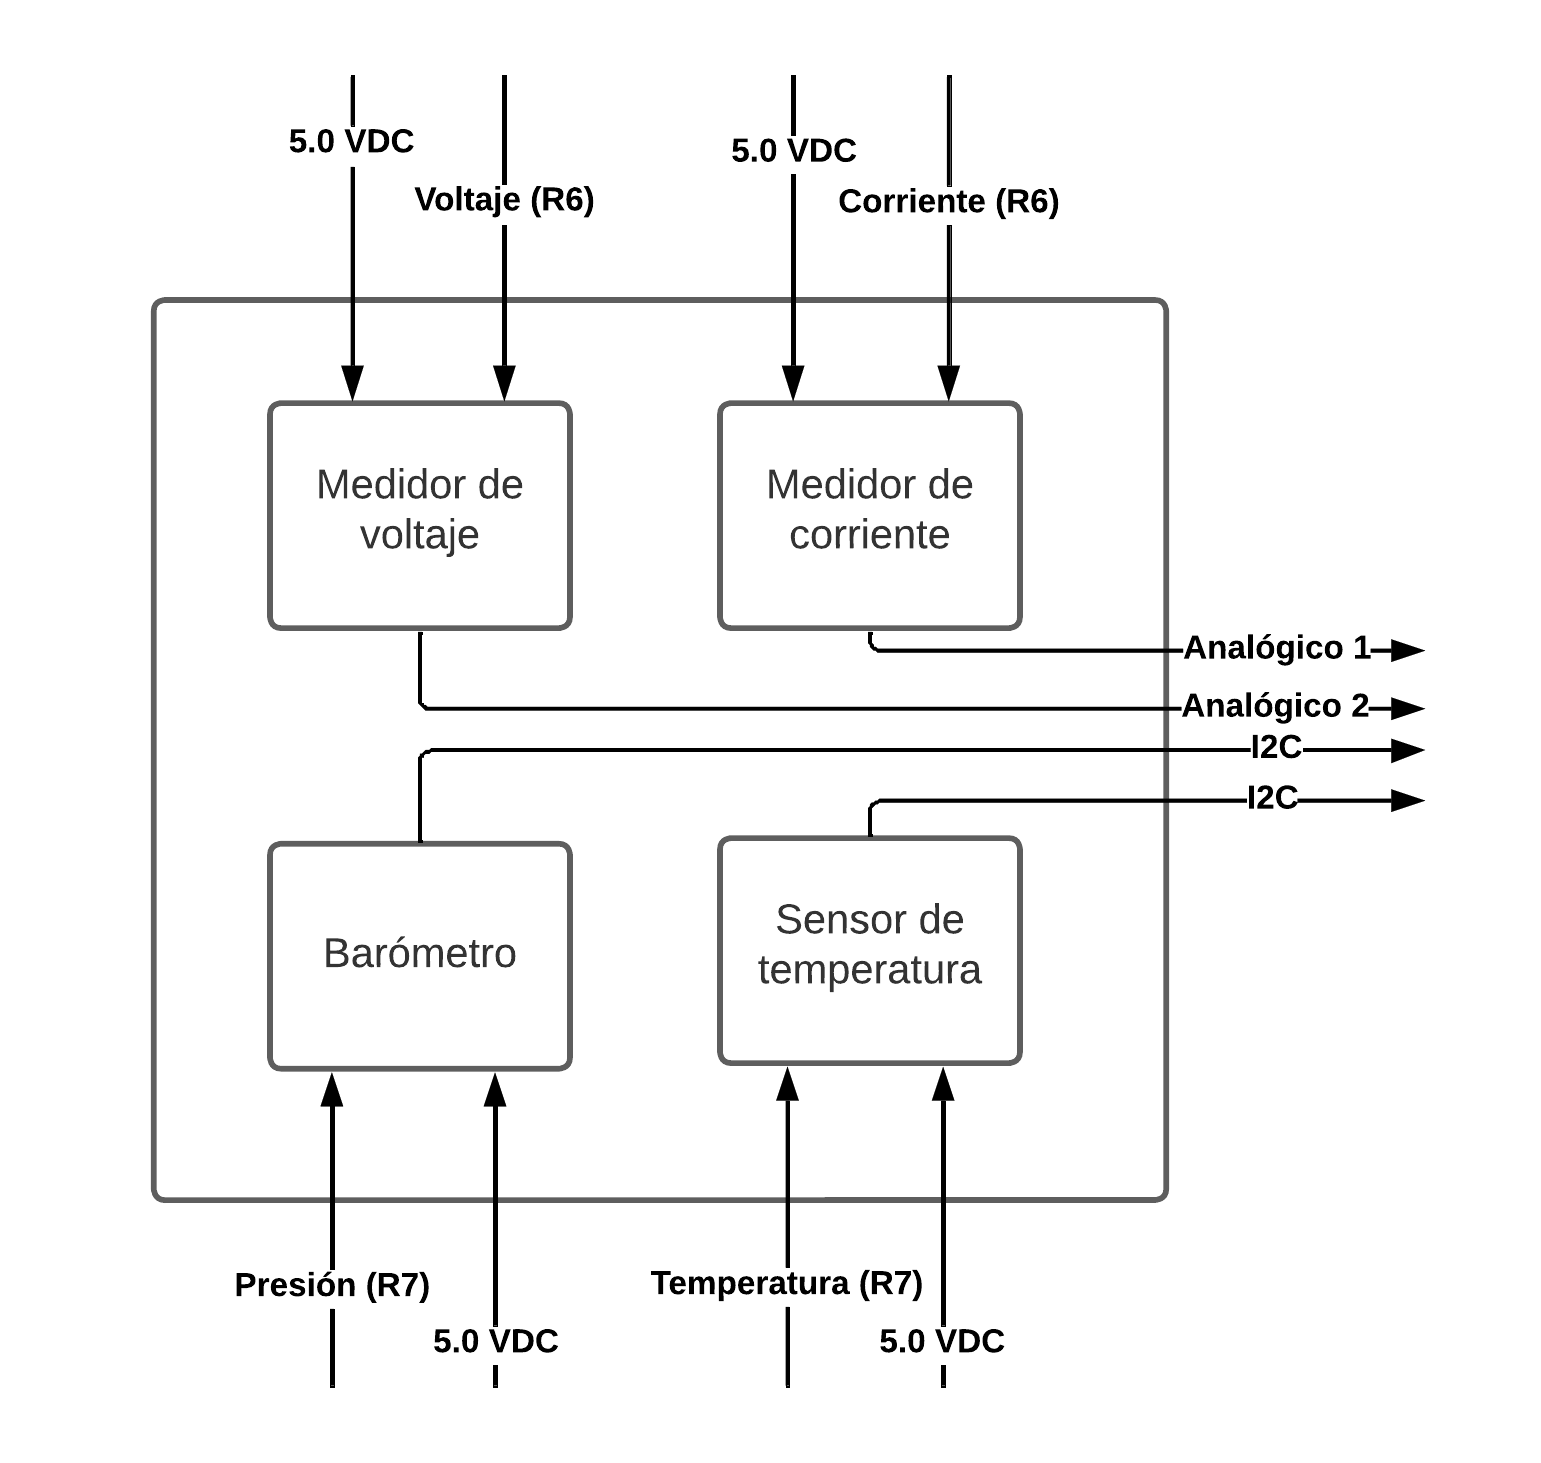
\includegraphics[width=\textwidth]{Pictures/Level2A.png}
\caption{Diagrama funcional Nivel 2, Instrumentación.}\label{fig:Level2A}
\index{figures}
\end{figure}

%**************************************
% BARÓMETRO

\begin{table}[h!]
    \centering
    \caption{Detalles de Nivel 1, Barómetro}
    \label{tab:nivel2_Barometro}
    \begin{tabular}{ll}
    \toprule
        Módulo  & Barómetro\\ 
    \midrule
        Entradas & 
        \begin{minipage}[t]{0.75\linewidth}
  - Alimentación $5.0 \, \text{V} \pm 1\%$\\
   - Presión atmosférica
 
        \end{minipage} \\
    \midrule
        Salidas & 
        \begin{minipage}[t]{0.75\linewidth}
    - Señal vía I2C

        \end{minipage} \\
    \midrule
        Funcionamiento & 
        \begin{minipage}[t]{0.75\linewidth}
El barómetro se alimenta con una tensión de $5.0 \, \text{V} \pm 1\%$. Transforma la presión atmosférica en una señal eléctrica, la acondiciona y posteriormente transmite los datos a través de la comunicación I2C.

        \end{minipage} \\
    \bottomrule
    \end{tabular}
\end{table}

%**************************************
% SENSOR DE TEMPERATURA 

\begin{table}[h!]
    \centering
    \caption{Detalles de Nivel 1, Sensor de temperatura}
    \label{tab:nivel2_Temperatura}
    \begin{tabular}{ll}
    \toprule
        Módulo  & Sensor de temperatura\\ 
    \midrule
        Entradas & 
        \begin{minipage}[t]{0.75\linewidth}
  - Alimentación $5.0 \, \text{V} \pm 1\%$\\
   - Temperatura ambiente
 
        \end{minipage} \\
    \midrule
        Salidas & 
        \begin{minipage}[t]{0.75\linewidth}
    - Señal vía I2C

        \end{minipage} \\
    \midrule
        Funcionamiento & 
        \begin{minipage}[t]{0.75\linewidth}
El sensor de temperatura se alimenta con una tensión de $5.0 \, \text{V} \pm 1\%$. Transforma la temperatura ambiente en una señal eléctrica, la acondiciona y posteriormente transmite los datos a través de la comunicación I2C.

        \end{minipage} \\
    \bottomrule
    \end{tabular}
\end{table}


%**************************************
% ADC

\begin{table}[h!]
    \centering
    \caption{Detalles de Nivel 1, Medidor de voltaje}
    \label{tab:nivel2_Voltaje}
    \begin{tabular}{ll}
    \toprule
        Módulo  & Medidor de voltaje\\ 
    \midrule
        Entradas & 
        \begin{minipage}[t]{0.75\linewidth}
  - Alimentación $5.0 \, \text{V} \pm 1\%$\\
   - Voltaje del banco de baterías
 
        \end{minipage} \\
    \midrule
        Salidas & 
        \begin{minipage}[t]{0.75\linewidth}
    - Señal analógica 2 - 10 bits.

        \end{minipage} \\
    \midrule
        Funcionamiento & 
        \begin{minipage}[t]{0.75\linewidth}
El ADC se alimenta con una tensión de $5.0 \, \text{V} \pm 1\%$. Este posee una resolución de 10 bits. 

        \end{minipage} \\
    \bottomrule
    \end{tabular}
\end{table}

%**************************************
% Sensor de corriente

\begin{table}[h!]
    \centering
    \caption{Detalles de Nivel 1, Medidor de corriente}
    \label{tab:nivel2_Voltaje}
    \begin{tabular}{ll}
    \toprule
        Módulo  & Medidor de corriente\\ 
    \midrule
        Entradas & 
        \begin{minipage}[t]{0.75\linewidth}
  - Alimentación $5.0 \, \text{V} \pm 1\%$\\
   - Corriente de banco de baterías.
 
        \end{minipage} \\
    \midrule
        Salidas & 
        \begin{minipage}[t]{0.75\linewidth}
    - Señal analógica 1.

        \end{minipage} \\
    \midrule
        Funcionamiento & 
        \begin{minipage}[t]{0.75\linewidth}
El medidor de corriente se alimenta con una tensión de $5.0 \, \text{V} \pm 1\%$. Utilizando el Efecto Hall, genera una señal de voltaje que se presenta como Analógica 1.


        \end{minipage} \\
    \bottomrule
    \end{tabular}
\end{table}
\chapter{Diseño e Implementación del Sistema}

En este capítulo, una vez que hemos definido la arquitectura del sistema y alcanzado un nivel funcional base que coincide con los componentes físicos (consulte las Figuras \ref{fig:Level1} y \ref{fig:Level2A}), nos sumergimos en la fase de diseño e implementación. A partir de la comprensión de las funciones esperadas en cada componente del sistema, desarrollaremos el diseño de circuitos electrónicos que, de manera coordinada, logren llevar a cabo el trabajo requerido. En este proceso, debemos tener en cuenta aspectos técnicos, así como limitaciones en el mercado, como la disponibilidad, los plazos de entrega y los costos. Por lo tanto, es responsabilidad del ingeniero establecer un diseño coherente que cumpla con los requisitos.

\hspace{1.27cm}Durante la selección de componentes, consideramos este proceso como una evaluación de valor, teniendo en cuenta la experiencia previa en trabajos anteriores. Esto aumenta la probabilidad de éxito de la misión, ya que estos componentes cuentan con un historial de éxitos en misiones aeroespaciales.

\newpage

% Cargador, baterias, protecciones eléctricas, reguladores de voltaje, Etapa de Potencia, Datalogger, Microcontrolador, Instrumentación (Barómetro, Medidor de voltaje, medidor de corriente, sensor de temperatura, Cámara IR).



\section{Microcontrolador}
sPara el control y procesamiento de datos en nuestro proyecto, hemos incorporado un Arduino Nano. El Arduino Nano es una placa de desarrollo de tamaño compacto que funciona como un microcontrolador programable. Está equipado con un microcontrolador ATmega328P y ofrece una amplia variedad de pines de entrada/salida, lo que facilita la conexión y control de sensores, actuadores y otros dispositivos periféricos. El Arduino Nano es conocido por su versatilidad y su capacidad para ejecutar programas personalizados, lo que lo convierte en una elección ideal para la implementación de lógica y control en nuestro sistema. Además, su tamaño compacto permite una integración eficiente en nuestra configuración de hardware \cite{arduino-nano} (ver Fig.\ref{fig:arduinoNanoBoard}). Las especificaciones del microcontrolador están disponible con más detalle en Tabla \ref{tab:nanotable}

\begin{figure}[hb!]
  \centering
  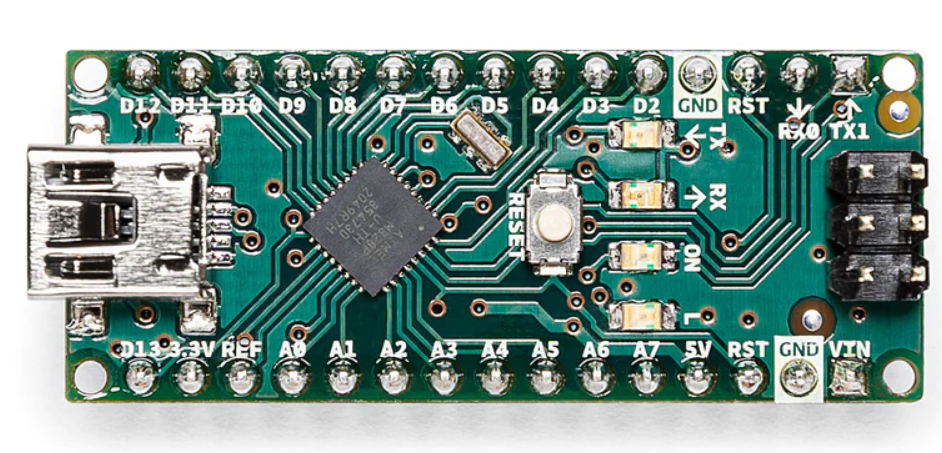
\includegraphics[width=0.4\linewidth]{Pictures/ArduinoNano.png} 
  \caption{Placa de desarrollo Arduino Nano}
  \label{fig:arduinoNanoBoard}
\end{figure}

\begin{table}[b]
\centering
\caption{Especificaciones del Microcontrolador AVR}
\label{tab:nanotable}
\begin{tabular}{l l}
\toprule % Línea horizontal superior
Característica & Valor \\
\midrule % Línea horizontal media
Arquitectura & AVR \\
Voltaje de operación & 5 V \\
Memoria Flash & 32 KB de los cuales 2 KB son utilizados por el bootloader \\
SRAM & 2 KB \\
Velocidad de reloj & 16 MHz \\
Pines de entrada analógica & 8 \\
EEPROM & 1 KB \\
Corriente por pines I/O  & 40 mA (Pines de E/S) \\
Voltaje de alimentación externa & 7-12V \\
Pines digitales I/O & 22 (6 de los cuales son PWM) \\
Salidas PWM  & 6 \\
Consumo de potencia & 19 mA \\
\bottomrule % Línea horizontal inferior
\end{tabular}
\end{table}

\newpage

\section{Datalogger}
Para el registro de datos, hemos optado por el módulo SparkFun OpenLog de código abierto. Este datalogger se comunica a través de una sencilla conexión serie y es compatible con tarjetas microSD de hasta 32 GB. Desempeña la función de un registro de datos, similar a una 'caja negra', capaz de almacenar información generada por nuestro sistema (ver Fig. \ref{fig:datalogger}). En el contexto del EPS, este módulo será responsable de almacenar datos eléctricos, como voltaje y corriente, así como datos ambientales, incluyendo temperatura y presión.

El módulo SparkFun OpenLog está equipado con un ATmega328 que opera a 16 MHz gracias a un oscilador incorporado. En modo inactivo, consume aproximadamente 2-3 mA cuando no hay datos que registrar. Durante una sesión de registro completa, el consumo de energía varía entre 10 y 20 mA, dependiendo del tipo de tarjeta microSD utilizada. Es compatible con tarjetas microSD que tienen una capacidad de 512 MB a 32 GB (ver Tabla \ref{tab:openlog_sparkfun_tabla_specs})\cite{sparkfun-13712}.



\begin{table}[h]
\centering
\caption{Especificaciones del SparkFun OpenLog}
\label{tab:openlog_sparkfun_tabla_specs}
\begin{tabular}{l l}
\toprule
Voltaje de operación & 3V a 5V \\
Velocidad del Microcontrolador & 16 MHz \\
Consumo en Modo Inactivo & 2-3 mA \\
Consumo durante Registro & 10-20 mA \\
Compatibilidad de Tarjetas microSD & 512 MB a 32 GB \\
Formatos de Tarjetas SD & FAT16 y FAT32 \\
\bottomrule
\end{tabular}
\end{table}


\begin{figure}[htbp]
  \centering
  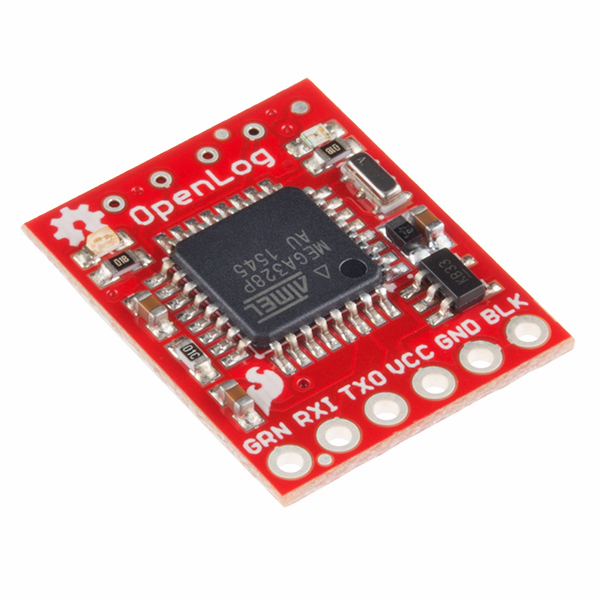
\includegraphics[width=0.4\linewidth]{Pictures/datalogger.jpg} 
  \caption{Módulo Datalogger Openlog de Sparkfun}
  \label{fig:datalogger}
\end{figure}


% Codigo de Prueba de Arduino IDE
\newpage
\begin{lstlisting}[caption={Prueba unitaria de Sparkfun Openlog desarrollado en Arduino IDE}, label={lst:ejemplo}]
#include <SoftwareSerial.h>

SoftwareSerial OpenLog(6, 5);

int statLED = 13;
float dummyVoltage = 3.50;

void setup() {
  pinMode(statLED, OUTPUT);
  Serial.begin(9600);
  OpenLog.begin(9600);

  Serial.println("This serial prints to the COM port");
  OpenLog.println("This serial records to the OpenLog text file");

  OpenLog.println("Hi there! How are you today?");
  OpenLog.print("Voltage: ");
  OpenLog.println(dummyVoltage);
  dummyVoltage++;
  OpenLog.print("Voltage: ");
  OpenLog.println(dummyVoltage);

  Serial.println("Text written to file. Go look!");
}
void loop() {
  digitalWrite(statLED, HIGH);
  delay(1000);
  digitalWrite(statLED, LOW);
  delay(1000);
}

}
\end{lstlisting}

% Codigo de Prueba de Arduino IDE 

\section{Etapa de Potencia}

Esta etapa incorpora un circuito de electrónica de potencia para gestionar la conexión y desconexión de cargas mediante señales digitales del microcontrolador. Se han establecido dos etapas de potencia: una para el bus de 3.3V, alimentando cargas descritas en la Tabla \ref{tab:cuadro_cargas_payload33}, y otra para el bus de 5.0V, para cargas detalladas en la Tabla \ref{tab:cuadro_cargas_payload50}

\begin{table}[h]
    \centering
    \renewcommand{\arraystretch}{1}
    \caption{Carga útil conectada a bus de 3.3v}
    \label{tab:cuadro_cargas_payload33}
    \begin{tabularx}{\textwidth}{lllllll}
    \hline
    \textbf{Descripción} & \textbf{Cantidad} & \textbf{I [mA]} & \textbf{P [W]} & \textbf{t [h]} & \textbf{E [Wh]} & \textbf{Q [mAh]} \\
    \hline
    \text{MCU 3} & 1 unidad & 70.00 & 0.23 & 2.00 & 0.46 & 140.00 \\ 
    \text{Cámara IR} & 1 unidad & 25.00 & 0.08 & 2.00 & 0.17 & 50.00 \\\hline 
    & \textbf{I Máx.} & \text{95.00} & & & & \textbf{190.00} \\ \hline
    \end{tabularx}
\end{table}

\begin{table}[h]
    \centering
    \renewcommand{\arraystretch}{1}
    \caption{Carga útil conectada a bus de 5.0v}
    \label{tab:cuadro_cargas_payload50}
    \begin{tabularx}{\textwidth}{lllllll}
        \hline
        \textbf{Descripción} & \textbf{Cantidad} & \textbf{I [mA]} & \textbf{P [W]} & \textbf{t [h]} & \textbf{E [Wh]} & \textbf{Q [mAh]} \\
        \hline
        Cámara & 1 unidad & 260.00 & 1.30 & 2.00 & 2.60 & 520 \\
        Datalogger 2 & 1 unidad & 12.00 & 0.06 & 2.00 & 0.12 & 24\\\hline
        ~ & \textbf{I Máx.} & \text{282.00} & ~ & ~ & ~ & \textbf{544.00} \\
        \hline
    \end{tabularx}
\end{table}

En el ámbito de la electrónica, las opciones de diseño abarcan soluciones que incorporan bobinas, como los relés y dispositivos semiconductores, como los transistores \cite{rashid2015electronica}. En el contexto de este trabajo de investigación, la elección de utilizar relés fue descartada debido a la significativa disipación de potencia por efecto Joule asociada con la operación de las bobinas. Esta decisión se respalda con ejemplos específicos de soluciones comerciales, como el relé PE014006, capaz de disipar hasta 209 mW \cite{TE2023PE014006}, un nivel de disipación que resulta inaceptable en aplicaciones alimentadas por baterías.


En consecuencia, dirigimos nuestra atención hacia alternativas basadas en semiconductores, específicamente los transistores. Entre estos, los BJT y los MOSFET son considerados mayoritariamente debido a su disponibilidad y asequibilidad. Mientras que el BJT es controlado por corriente, el MOSFET responde al control por voltaje. Las diferencias fundamentales entre estos dispositivos se resumen de manera concisa en la Tabla \ref{tab:comparisonbjtmosfet}.

Con el objetivo de realizar un análisis más directo y preciso, optamos por dos modelos comerciales accesibles: el BJT 2N2222A (Fig. \ref{fig:subfig12N2222A}) y el MOSFET BS170 (Fig. \ref{fig:subfig2bs170}).
\newpage

\begin{table}[h]
    \centering
    \renewcommand{\arraystretch}{1.5}
    \begin{tabular}{p{0.35\linewidth}p{0.25\linewidth}p{0.30\linewidth}}
    \hline
        \textbf{Característica} & \textbf{BJT} & \textbf{MOSFET} \\ \hline
        Tipo & PNP/NPN & N/P \\ 
        Control & Corriente & Voltaje \\ 
        Temp. Coeficiente & Negativo & Positivo \\ 
        Salida controlada & Corriente de base & Voltaje en compuerta\\ 
        Costo & Bajo & Alto \\ 
        Descarga electrostática & No problema & Problema potencial \\ 
        Ganancia de corriente & Baja e inestable & Alta y estable \\ 
        Resistencia de entrada & Baja & Alta \\ 
        Corriente de entrada & mA/uA & pA \\ 
        Velocidad de conmutación & Más lenta & Más rápida \\ 
        Impedancia de entrada & Baja & Alta \\ 
        Frecuencia de conmutación & Baja & Alta \\ 
        Aplicaciones & Baja corriente & Alta corriente \\ \hline
    \end{tabular}
    \caption{Características generales de BJT y MOSFET.}
    \label{tab:comparisonbjtmosfet}
\end{table}

\vspace{1 cm}

\begin{figure}[h]
  \centering
  \begin{subfigure}{0.4\textwidth}
    \centering
    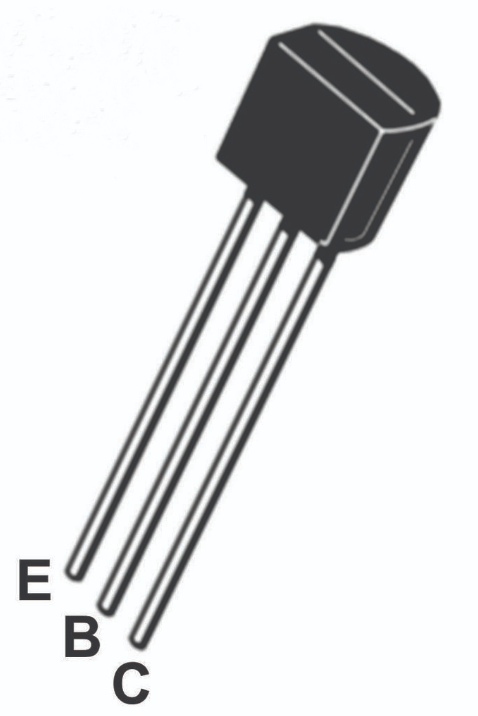
\includegraphics[width=0.7\linewidth]{Pictures/2N2222A_Pinout.png}
    \caption{BJT 2N2222A}
    \label{fig:subfig12N2222A}
  \end{subfigure}
  \hspace{2cm} % Ajusta el espacio entre las subfiguras
  \begin{subfigure}{0.4\textwidth}
    \centering
    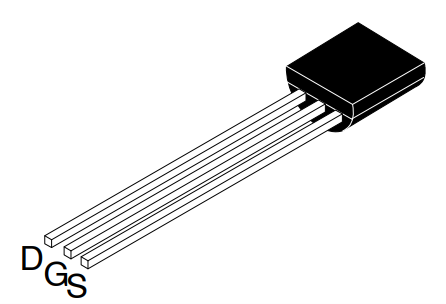
\includegraphics[width=0.9\linewidth]{Pictures/BS170_Pinout.png}
    \caption{MOSFET BS170}
    \label{fig:subfig2bs170}
  \end{subfigure}
  \caption{Transistores BJT y MOSFET comerciales}
  \label{fig:arduinoNanoSubfigures}
\end{figure}

\newpage

\subsection{Análisis Comparativo entre BJT 2N2222A y MOSFET BS170}

Con el objetivo de realizar una comparación precisa entre los transistores BJT 2N2222A y MOSFET BS170, es imperativo establecer criterios relevantes que orienten la evaluación:

\begin{itemize}
\item Capacidad de corriente en drenaje o colector.
\item Rango de temperatura de operación.
\item Potencia disipada.
\item Resistencia térmica.
\end{itemize}

Para facilitar la elaboración de una tabla comparativa directa entre ambos modelos, nos apoyaremos en las hojas técnicas respectivas proporcionadas en \cite{BS170Datasheet} y \cite{2N2222A_Datasheet}.

\begin{table}[h]
    \centering
    \begin{tabularx}{\textwidth}{lcc}
        \hline
        \textbf{Parámetro} & \textbf{BS170} & \textbf{2N2222A} \\ 
        \hline
        Corriente Máxima ($I_{\text{Máx.}}$) & \SI{500}{\milli\ampere} & \SI{600}{\milli\ampere} \\ 
        Potencia Disipada ($P_D$) & \SI{830}{\milli\watt} a \SI{6.60}{\milli\watt/\celsius} & \SI{625}{\milli\watt} a \SI{5.0}{\milli\watt/\celsius} \\ 
        Potencia Disipada ($P_D$) & \SI{830}{\milli\watt} a \SI{6.60}{\milli\watt/\celsius}  & \SI{1.5}{\watt} a \SI{12.0}{\milli\watt/\celsius} \\ 
        Rango de Temperatura & \SI{-55}{\celsius} a \SI{+150}{\celsius} & \SI{-55}{\celsius} a \SI{+150}{\celsius} \\ 
        R$\theta$ja & \SI{150}{\celsius/\milli\watt} & \SI{200}{\celsius/\milli\watt} \\ 
        \hline
    \end{tabularx}
    \caption{Comparativa entre MOSFET BS170 y BJT 2N2222A.}
    \label{tab:comparisonmodeltransistor}
\end{table}

En la Tabla \ref{tab:comparisonmodeltransistor} se detallan las características clave de los modelos de transistores seleccionados. El BJT 2N2222A, al ser un dispositivo de coeficiente térmico negativo (NTC), muestra incremento en la resistencia interna con la disminución de la temperatura ambiente (Fig. \ref{fig:pdenviromentaltemperature}). En contraste, los transistores MOSFET, como el BS170, son PTC y disminuyen su resistencia a bajas temperaturas (Fig. \ref{fig:resinternavscorriente}).

Ambos transistores admiten un amplio rango de temperaturas, pero el BJT permite una corriente más alta y tiene un incremento térmico significativamente mayor. Sin embargo, considerando el consumo de energía crítico para baterías, la respuesta más eficiente del MOSFET a la temperatura lo posiciona como la mejor alternativa.

En conclusión, para la aplicación específica en la misión de globo de gran altitud de StratoBalloon, se favorece la implementación del MOSFET BS170 en la etapa de potencia, debido a su eficiencia energética y respuesta térmica más favorable.

\newpage

\begin{figure}[h]
  \centering
  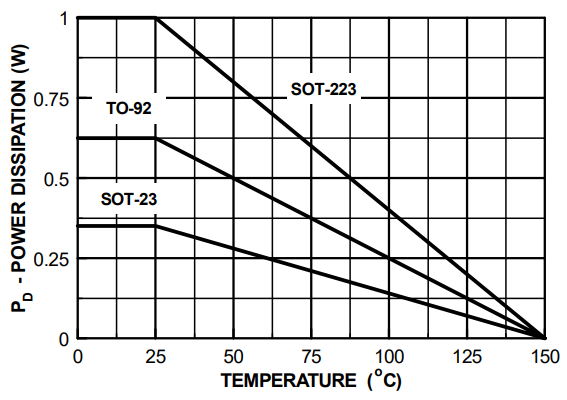
\includegraphics[width=0.85\linewidth]{Pictures/2N2222ApowerD.png} 
  \caption{Variación de la Potencia Disipada en el 2N2222A en Función de la Temperatura Ambiente \cite{2N2222A_Datasheet}}
  \label{fig:pdenviromentaltemperature}
\end{figure}

\begin{figure}[h]
  \centering
  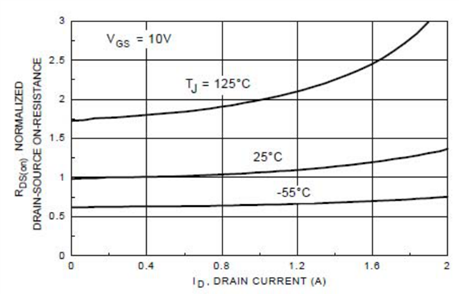
\includegraphics[width=0.9\linewidth]{Pictures/resvscorriente.png} 
  \caption{Variación de la Resistencia Interna en Función de la Corriente a Distintas Temperaturas Ambiente para un MOSFET BS170 \cite{BS170Datasheet}}
  \label{fig:resinternavscorriente}
\end{figure}

\newpage

\subsection{Diseño e implementación de MOSFET BS170}
    

Considerando las indicaciones del fabricante \cite{BS170Datasheet}, se han identificado parámetros fundamentales para el diseño de la etapa de potencia con el MOSFET BS170. Destaca el voltaje máximo $V_{DS}$ entre Drenaje y Fuente, limitado a 60 V, así como el máximo voltaje $V_{GS}$ soportado en la compuerta, establecido en 20 V.

Un aspecto clave es $V_{GS}(TH)$, definiendo el rango típico de voltajes para activar la compuerta y permitir la conducción, sujeto a una curva de comportamiento en relación con la corriente en el Drenaje2. Además, se aborda $I_{D}(Load) Máx$, indicando la corriente máxima en el Drenaje, asociada con la carga máxima manejable.

Estos aspectos esenciales se detallan en la Tabla \ref{tab:Designbs170}, proporcionando información crucial para un diseño eficiente y seguro de la etapa de potencia.

\begin{table}[!ht]
    \centering
    \begin{tabular}{l l}
    \hline
        \textbf{Parámetro} & \textbf{Valor} \\ \hline
        V\_DS (BR) & 60 V \\ 
        V\_GS  MAX & 20 V \\ 
        V\_GS Threshold & Min. 0.8 – 2.1 avg – 3 Máx \\ 
        I\_D (Load) MAX & 500 mA \\ 

        I\_DSS & 10 nA \\ 
        I\_DM & 1200 mA \\ 
    \hline
    \end{tabular}
    \caption{Parámetros de diseño para MOSFET BS170}
    \label{tab:Designbs170}
\end{table}

De acuerdo a la documentación técnica del MOSFET BS170 \cite{BS170Datasheet}, y basándonos en la Figura \ref{fig:bs170vgsidrainA}, seleccionamos el valor mínimo de $V_{GS}$ necesario para el BS170 en el bus de 3.3 V, considerando una corriente aproximada de 100 mA. Asimismo, elegimos el voltaje mínimo $V_{GS}$ para la etapa de potencia en el bus de 5.0 V, con una corriente mínima de 300 mA. En ambos casos, y al verificar que los valores son aceptables según se muestra en la Tabla \ref{tab:Designbs170}, optamos por utilizar el voltaje suministrado naturalmente por el Arduino Nano, que es de 5 VDC con una corriente máxima continua de 20 mA \cite{arduino_getting_started}.

Dicho esto, siguiendo la conexión del MOSFET en la configuración "low side" para este MOSFET de canal N, permitiendo así que funcione como un interruptor normalmente abierto y se active en función de una señal de entrada del microcontrolador, el esquemático y vista 3D de la PCB resultante se muestran en la Figura \ref{fig:combined_figureBS170}.

\newpage

\begin{figure}[h]
  \centering
  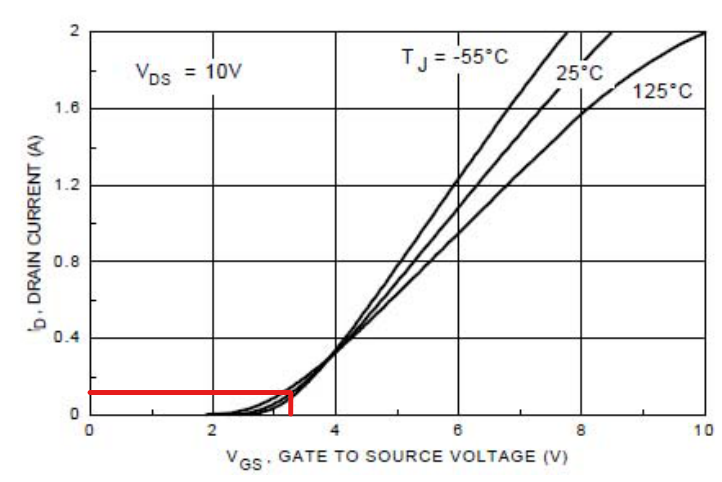
\includegraphics[width=0.45\linewidth]{Pictures/33busvgsgraphic.png} 
  \caption{$V_{GS}$ para bus de 3.3 V a 100 [mA]. \cite{BS170Datasheet}}
  \label{fig:bs170vgsidrainA}
\end{figure}

\begin{figure}[h]
  \centering
  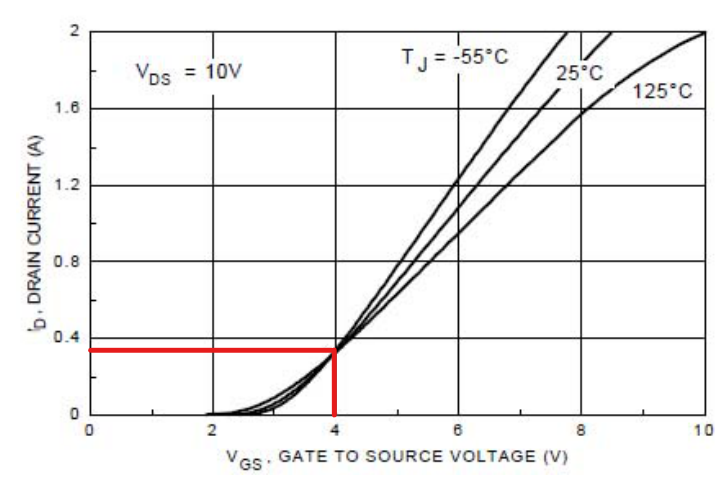
\includegraphics[width=0.45\linewidth]{Pictures/50busvgsgraphic.png} 
  \caption{$V_{GS}$ para bus de 5.0 V a 300 [mA]. \cite{BS170Datasheet}}
  \label{fig:bs170vgsidrainB}
\end{figure}

\vspace{1 cm }

\begin{figure}[h]
    \centering
    \begin{subfigure}{0.45\textwidth}
        \centering
        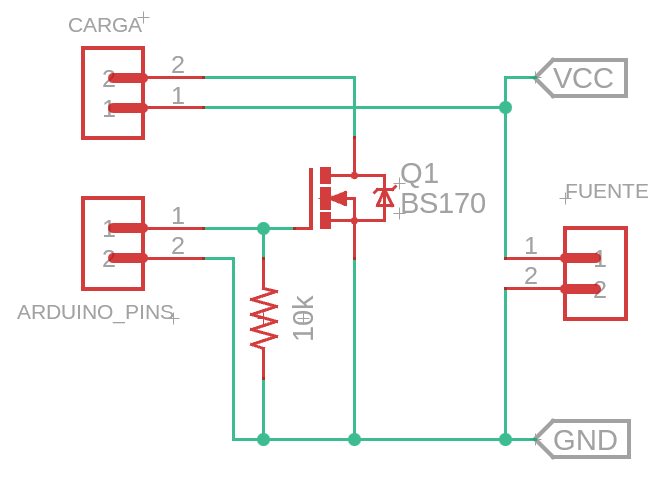
\includegraphics[width=\linewidth]{Pictures/EtapaMosfet_Esquematico.png}
        \caption{Esquemático de la etapa de potencia con MOSFET BS170. La resistencia de 10k ohmios es un valor recomendado por el fabricante \cite{BS170Datasheet}.}
        \label{fig:Esquematico_powerstage170}
    \end{subfigure}
    \hfill
    \begin{subfigure}{0.45\textwidth}
        \centering
        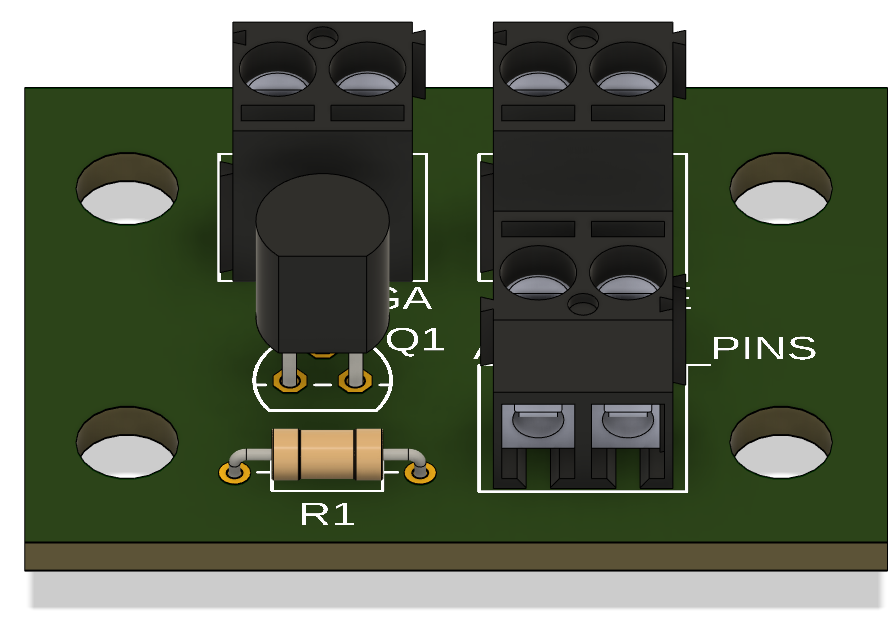
\includegraphics[width=\linewidth]{Pictures/3D_MOSFET.png}
        \caption{Vista 3D de la etapa de potencia con MOSFET BS170.}
        \label{fig:3Do_powerstage170}
    \end{subfigure}
    \caption{Esquemático y vista 3D de la etapa de potencia con MOSFET BS170.}
    \label{fig:combined_figureBS170}
\end{figure}


\newpage


\section{Instrumentación}

\subsection{Barómetro y sensor de temperatura}

Para llevar a cabo la medición de presión y temperatura durante la misión, así como para realizar un análisis comparativo con respecto al rendimiento frente a parámetros eléctricos, hemos optado por la utilización del sensor de bajo costo MS5611. Las especificaciones detalladas de este sensor se presentan en la Tabla \ref{tab:ms5611}.

El código de programación utilizado para realizar la prueba unitaria de este componente se encuentra detallado en el Código 4.2.


\begin{table}[h]
\centering
\caption{Especificaciones sensor MS5611}
\label{tab:ms5611}
\begin{tabular}{ll}
\toprule
Rango de presiones & 10 to 1200 mbar \\
Rango de temperaturas & -40 °C to 85 °C \\
Resolución en altura & 10 cm \\
Resolución en presión & 0.012 mbar \\
Resolución en temperatura & 0.01 °C \\
Fuente de alimentación & 1.8 to 3.6 V \\
Consumo en corriente & 1.4 mA \\
Comunicación & I²C y SPI \\
\bottomrule
\end{tabular}
\end{table}

% Codigo de Prueba de Arduino IDE

\begin{lstlisting}[caption={Prueba unitario en sensor MS5611 desarrollado en Arduino IDE}, label={code:ms5611cod}]
#include <Wire.h>
#include <MS5611.h>

MS5611 ms5611;
double referencePressure;

void setup() 
{
  Serial.begin(9600);
  Serial.println("Initialize MS5611 Sensor");
  
  while (!ms5611.begin())
  {
    Serial.println("Could not find a valid MS5611 sensor, check wiring!");
    delay(500);
  }
  
  referencePressure = ms5611.readPressure();
  checkSettings();
}

void checkSettings()
{
  Serial.print("Oversampling: ");
  Serial.println(ms5611.getOversampling());
}

void loop()
{
  uint32_t rawTemp = ms5611.readRawTemperature();
  uint32_t rawPressure = ms5611.readRawPressure();
  
  double realTemperature = ms5611.readTemperature();
  long realPressure = ms5611.readPressure();
  
  float absoluteAltitude = ms5611.getAltitude(realPressure);
  float relativeAltitude = ms5611.getAltitude(realPressure, referencePressure);
  
  String logData = String(realTemperature, 2) + " *C, " + String(realPressure) + " Pa; ";
  logData += "Absolute Altitude: " + String(absoluteAltitude, 2) + " m; ";
  
  Serial.println(logData);
  delay(1000);

}
\end{lstlisting}

% Codigo de Prueba de Arduino IDE 


\subsection{Medidor de voltaje}

Para medir los voltajes del banco de baterías del Sistema de energía (EPS), hemos elegido utilizar el Convertidor Analógico-Digital (ADC) integrado en el Arduino Nano. El ADC del Arduino Nano ofrece una resolución de 10 bits, lo que permite mediciones precisas con una sensibilidad de 4.88 mV por unidad de conteo (4.88 mV/count). A continuación, presentamos un código de prueba unitaria para la medición de voltajes (ver Código 4.3). Los parámetros técnicos asociados al ADC se detallan en Tabla \ref{tab:ArduinoADC}.

\begin{table}[h]
\centering
\caption{Especificaciones del ADC del Arduino Nano}
\label{tab:ArduinoADC}
\begin{tabular}{llll}
\toprule
\textbf{Placa} & \textbf{Voltaje de Operación} & \textbf{Pines} & \textbf{Resolución Máx.} \\
\midrule
Nano & 5 Voltios & A0 a A5 & 10 bits \\
\bottomrule
\end{tabular}
\end{table}


% Codigo de Prueba de Arduino IDE

\begin{lstlisting}[caption={Prueba unitaria para ADC desarrollado en Arduino IDE}, label={lst:ADCode}]
const int pinAnalogico = A0;

void setup() {
  Serial.begin(9600);
}

void loop() {
  int lectura = analogRead(pinAnalogico);
  float voltaje = (lectura * 5.0) / 1023.0;

  Serial.print("Valor: ");
  Serial.print(lectura);
  Serial.print(", Voltaje: ");
  Serial.println(voltaje, 2);

  delay(1000);
}

\end{lstlisting}

% Codigo de Prueba de Arduino IDE 

\newpage
\subsection{Medidor de corriente}

Para la medición precisa de corriente sin afectar el circuito, hemos optado por el uso del sensor ACS723 (ver Fig.\ref{fig:Sensor_ACS723_Imagen} ), una placa de alta precisión diseñada para aplicaciones de corriente AC y DC, que utiliza el efecto Hall para generar una tensión proporcional a la corriente que fluye a través de sus pines IP+ e IP-. Una ventaja fundamental es que el sensor emplea un efecto Hall, lo que proporciona un aislamiento eléctrico entre el circuito medido y el circuito que lee el sensor. Esto significa que, aunque nuestro Arduino funcione a 5V, el circuito medido puede operar a tensiones DC o AC más elevadas.

\begin{figure}[h]
  \centering
  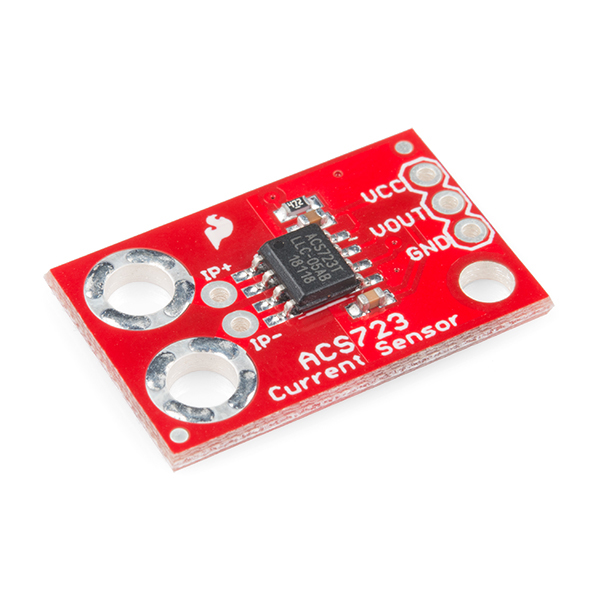
\includegraphics[width=0.7\linewidth]{Pictures/ACS723.jpg} 
  \caption{Sensor ACS723 de Sparkfun.}
  \label{fig:Sensor_ACS723_Imagen}
\end{figure}


Este sensor de baja corriente puede detectar corrientes muy pequeñas, incluso a partir de 10mA, y corrientes más altas de hasta 5A. No obstante, dado que su salida es analógica, la precisión de las lecturas estará limitada por el ruido y la resolución del convertidor analógico-digital (ADC) que lee la señal. Además, esta placa ofrece aislamiento eléctrico completo entre los circuitos medidos y de detección y, gracias a un amplificador integrado, permite ajustar su sensibilidad \cite{sparkfun14544}.

A continuación, presentamos un código de prueba unitaria para la medición de corrientes utilizando este dispositivo (ver Código 4.4).


% Codigo de Prueba de Arduino IDE

\begin{lstlisting}[caption={Prueba unitaria para sensor de corriente ACS723}, label={lst:acs723cod}]

const int analogInPin = A0;
const int avgSamples = 10;
int sensorValue = 0;
float sensitivity = 100.0 / 500.0; 
float Vref = 2500;

void setup() {
  Serial.begin(9600);
}

void loop() {
  for (int i = 0; i < avgSamples; i++) {
    sensorValue += analogRead(analogInPin);
    delay(2);
  }
  sensorValue = sensorValue / avgSamples;

  float voltage = 4.88 * sensorValue;
  float current = (voltage - Vref) * sensitivity;

  Serial.print(current);
  Serial.print("mA");
  Serial.print(analogRead(A1));
  Serial.print("mV_Resistor");

  Serial.print("\n");
  
  sensorValue = 0;
}


\end{lstlisting}

% Codigo de Prueba de Arduino IDE 

\newpage



\section{Baterías}

La selección de baterías de iones de litio comerciales (COTS, por sus siglas en inglés) adecuadas para misiones en globos de gran altitud es una consideración crítica. Si bien las baterías COTS ofrecen rentabilidad, amplia disponibilidad y un historial probado en diversas aplicaciones, se deben abordar cuidadosamente los desafíos únicos de operar a altitudes extremas. Las misiones en globos de gran altitud requieren un rendimiento confiable de las baterías, incluso bajo condiciones ambientales adversas e impredecibles.

Las bajas temperaturas y presiones pueden afectar significativamente el rendimiento de las baterías, comprometiendo potencialmente la seguridad de la misión. Operar baterías en tales condiciones conlleva efectos perjudiciales, incluyendo la alteración de la conductividad iónica, la resistencia interna y la cinética de transferencia de carga\cite{Ma2018,Navarathinam2011}. Dada la importancia de la energía de la batería para los sistemas electrónicos durante las misiones en globos de gran altitud, evaluar las baterías de iones de litio COTS es esencial para garantizar el éxito de la misión.

\subsection{Química y geometría de las baterías}\label{AA} 

A pesar de su tamaño compacto, alta densidad de energía y baja tasa de autodescarga, las baterías de iones de litio conllevan riesgos potenciales inherentes, como posibles incendios o explosiones debido a cortocircuitos internos \cite{Meyer2020}.

En cuanto a la geometría de la batería, los diseños prismáticos optimizan la utilización del espacio, pero a menudo requieren mejoras en la eficiencia térmica. Las baterías de tipo bolsa ofrecen flexibilidad en su forma, aunque necesitan un soporte adecuado. Por otro lado, las baterías cilíndricas, como las del tipo 18650, proporcionan estabilidad mecánica y cuentan con sistemas de seguridad integrados, lo que las hace especialmente adecuadas para aplicaciones en globos de gran altitud\cite{Eleazar2020}.

\subsection{Baterías comerciales}

\vspace{0.5cm}
\begin{figure}[htbp]
  \centering
  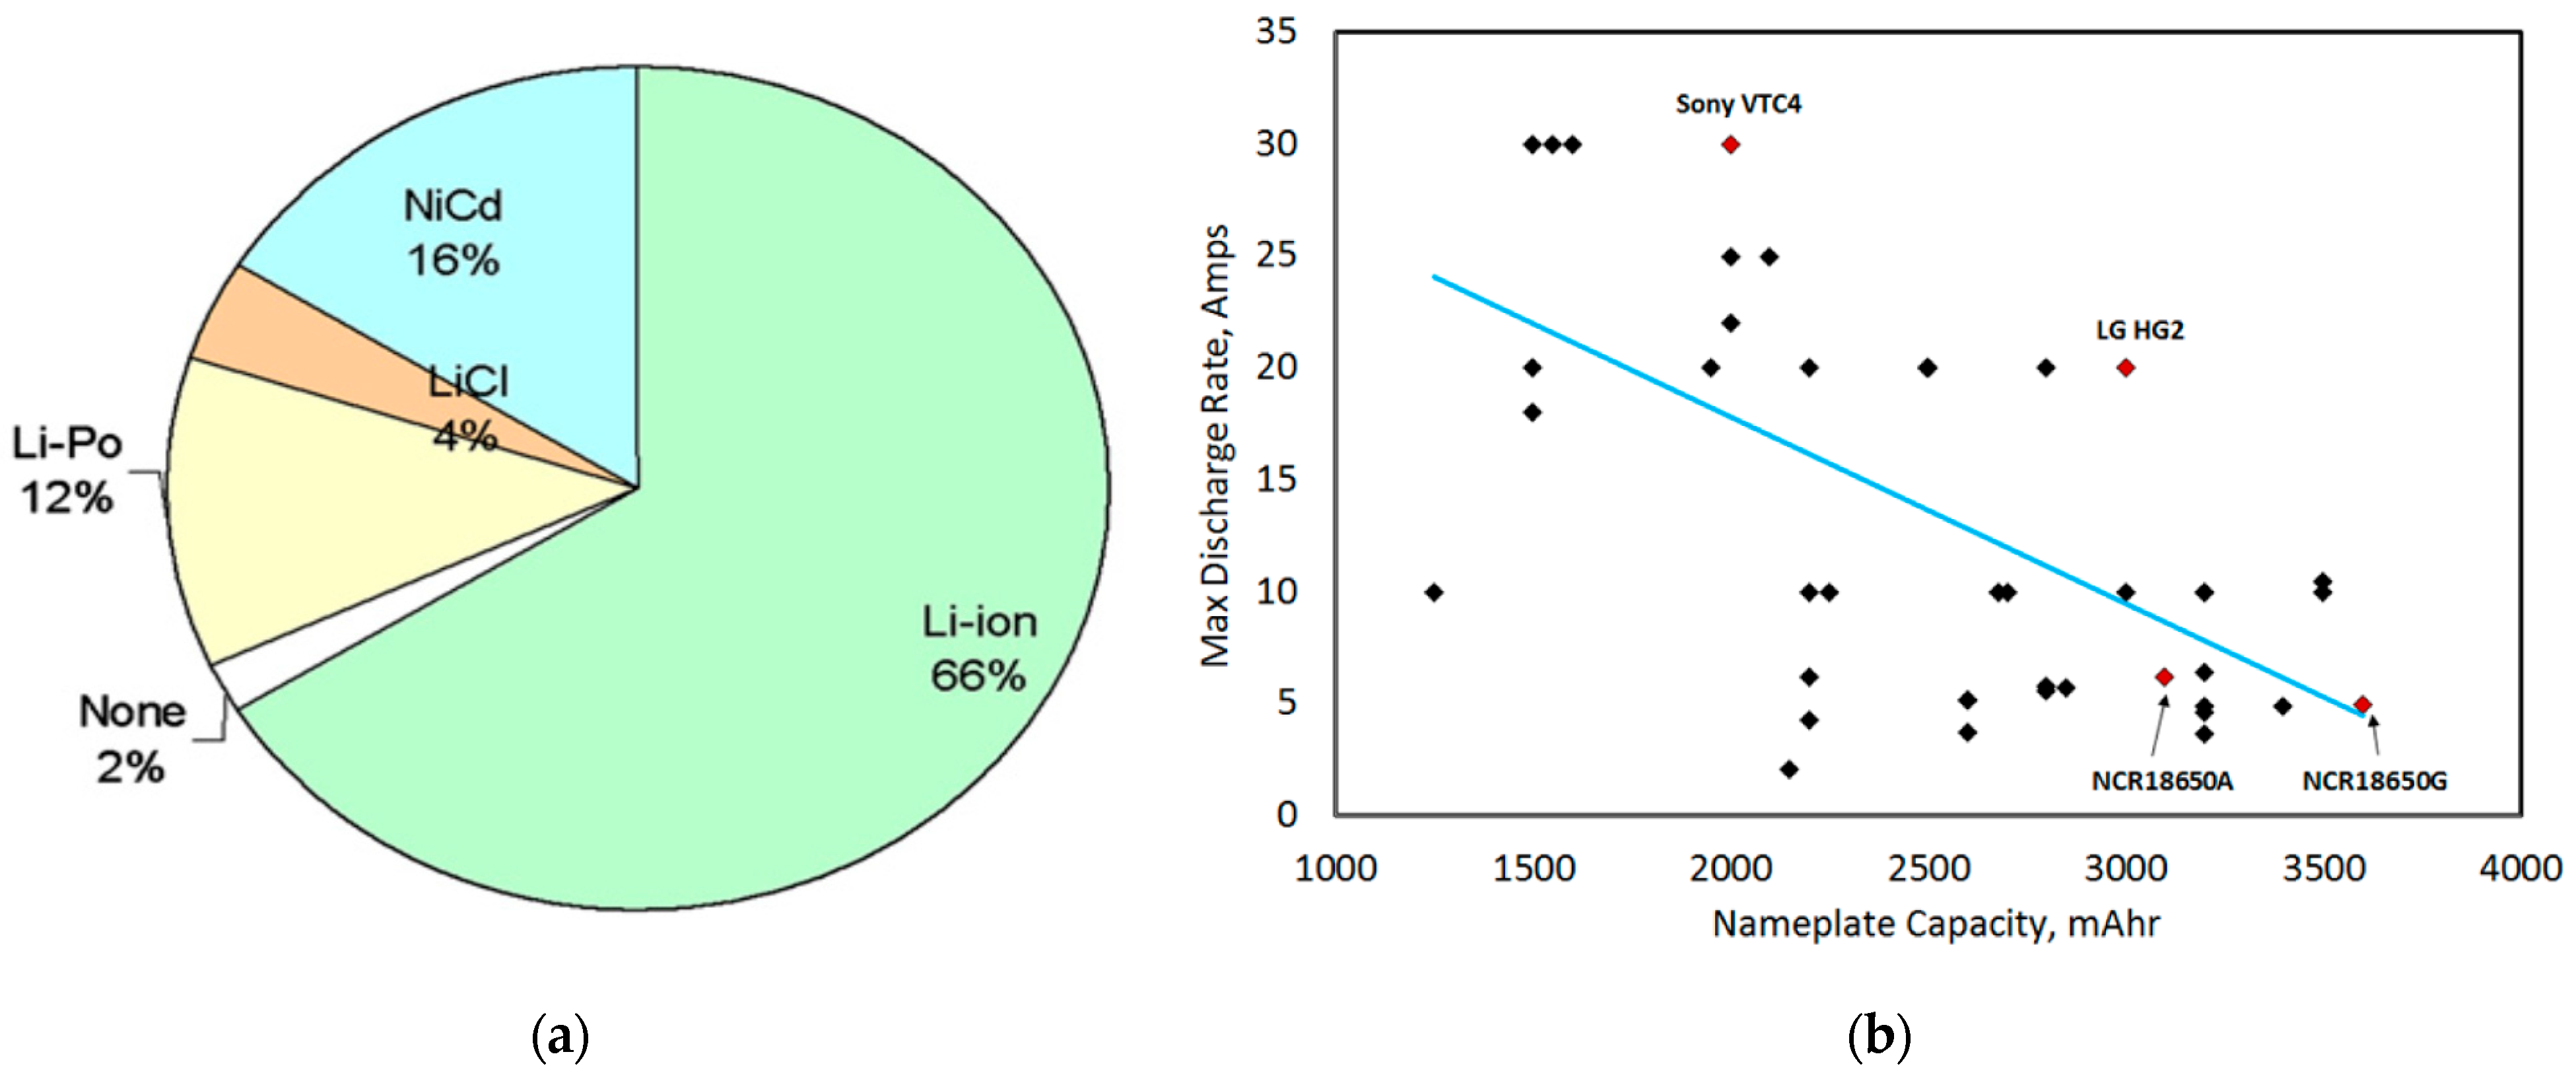
\includegraphics[width=0.9\linewidth]{Pictures/COTSBatteries.png} 
  \caption{(a) Battery types used in pico- and nano-satellites\cite{bouwmeester2010survey}.
  (b) Summary of maximum discharge rate capabilities versus nameplate capacity of some representative COTS 18650 Li-ion cells \cite{chin2018energy}}
  \label{fig:graphicsCOTS}
\end{figure}

Basándonos en el estudio exhaustivo realizado en \cite{Knap2020} y representado en la Fig. \ref{fig:graphicsCOTS}, el rendimiento de las celdas de iones de litio puede ser efectivamente limitado por tres modelos específicos: Sony VTC4, LG HG2 y Panasonic NCR18650G.

Debido a su costo asequible, historial comprobado de confiabilidad y características electroquímicas de carga y descarga, hemos optado por utilizar la batería Panasonic NCR18650B en este trabajo. \newpage Esta batería tiene una capacidad de descarga de hasta 4.9A, una capacidad de carga de 3400 mAh y un rango de temperatura de -20 a 60 grados Celsius\cite{panasonic_18650b}. Además, cuenta con documentación técnica que respalda su uso en aplicaciones aeroespaciales previas\cite{Knap2020}\cite{Kumar2022}.

\subsection{Arreglo para el banco de baterías}

Al analizar la Tabla \ref{tab:requerimientos-eps}, que presenta los requerimientos del Sistema de Energía (EPS), obtenidos a partir del presupuesto energético desarrollado en las Tablas \ref{tab:cuadro-cargas1} y \ref{tab:cuadro-cargas2}, se observa que la corriente requerida por las cargas se estima en 1385.4 mA. Tras consultar la hoja técnica del modelo de batería Panasonic NCR18650B utilizado en este trabajo, se verifica que este modelo de batería puede suministrar una corriente máxima de 4.9 A. Por lo tanto, este diseño no está restringido ni obligado a utilizar arreglos en paralelo.

En lo que respecta a las necesidades de capacidad de carga, se ha estimado un valor nominal de 6844.2 mAh para la misión StratoBalloon, sin considerar las posibles pérdidas en las diversas etapas del EPS.

Dado que la capacidad nominal de esta batería es de 3400 mAh, se calcula que se requerirían 3 baterías, considerando un redondeo hacia arriba. No obstante, dado que aún disponemos de espacio y pensando en futuras aplicaciones, hemos decidido utilizar 4 baterías de este tipo.

Con el fin de explorar el funcionamiento de etapas posteriores, como los convertidores DC-DC, se han considerado tres diseños: 4s1p (Fig. \ref{fig:powerbank}), 2s2p (Fig. \ref{fig:powerbank2}) y 1s4p (Fig. \ref{fig:powerbank3}).

\begin{figure}[h]
  \centering
  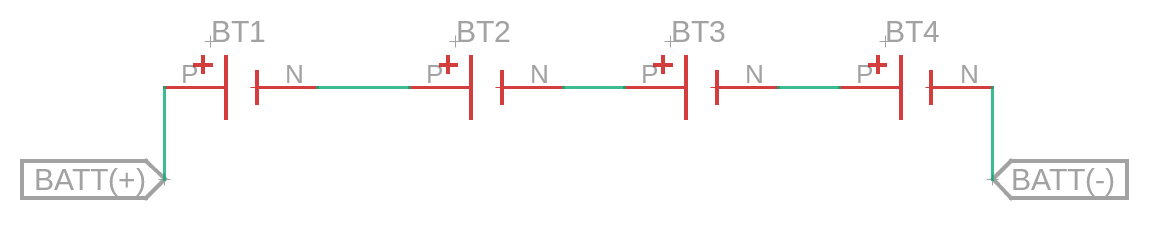
\includegraphics[width=0.7\linewidth]{Pictures/PowerBank.png} 
  \caption{Banco de baterías en arreglo 4s1p a 14.4 V.}
  \label{fig:powerbank}
\end{figure}

\begin{figure}[h]
  \centering
  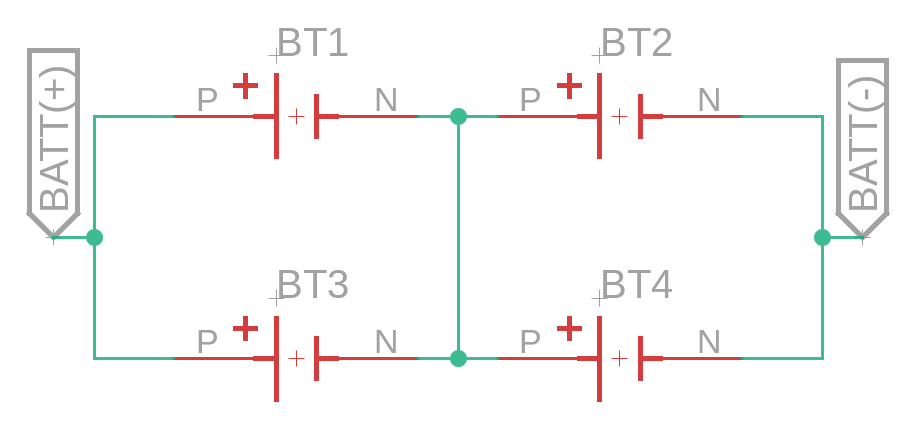
\includegraphics[width=0.5\linewidth]{Pictures/Batteries2s2p.png} 
  \caption{Banco de baterías en arreglo 2s2p a 7.2 V.}
  \label{fig:powerbank2}
\end{figure}

\begin{figure}[h]
  \centering
  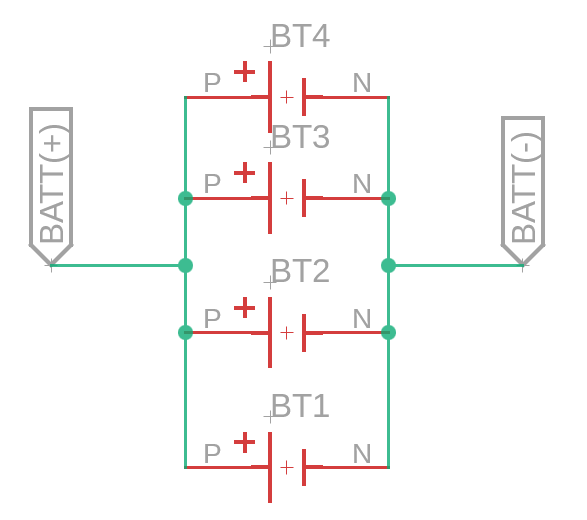
\includegraphics[width=0.4\linewidth]{Pictures/Batteries1s4p.png} 
  \caption{Banco de baterías en arreglo 1s4p a 3.6 V.}
  \label{fig:powerbank3}
\end{figure}

\begin{figure}
  \centering
  \begin{subfigure}{0.35\linewidth}
    \centering
    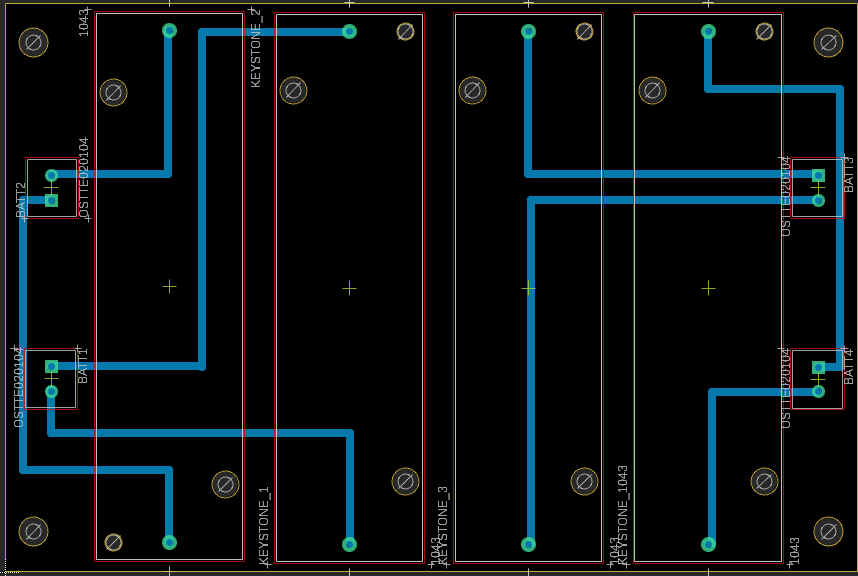
\includegraphics[width=\linewidth]{Pictures/DesignPCBHolders.png}
    \caption{Diseño de pistas}
    \label{fig:powerbankpistas}
  \end{subfigure}
  \begin{subfigure}{0.45\linewidth}
    \centering
    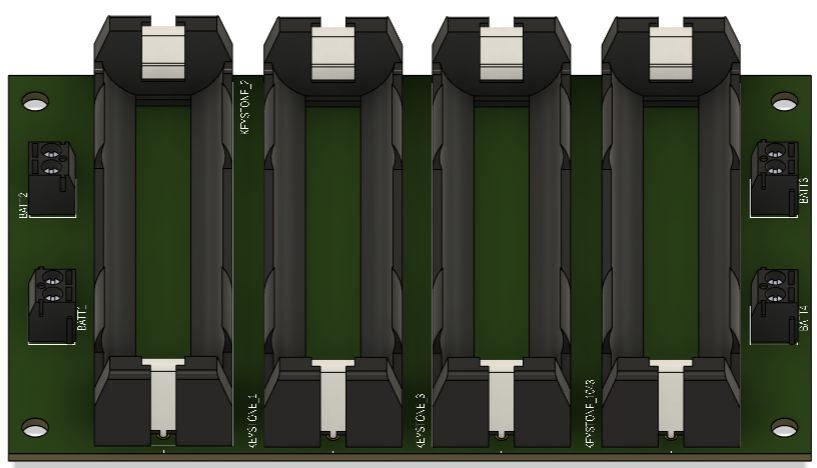
\includegraphics[width=\linewidth]{Pictures/DesignPCBHolders3d.png}
    \caption{Vista 3D de PCB}
    \label{fig:powerbankpistas3d}
  \end{subfigure}
  \caption{Banco de baterías}
  \label{fig:powerbank-subfiguras}
\end{figure}


Para llevar a cabo pruebas preliminares y verificar el rendimiento óptimo en prototipado rápido, hemos instalado en una placa de circuito impreso (PCB) cuatro pilas a través de los portadores Keystone 1043 conectados a bornes para facilitar su manipulación (consulte las Fig. \ref{fig:powerbankpistas} y \ref{fig:powerbankpistas3d}).


\section{Selección del Cargador para el Sistema de Energía (EPS)}

Una vez determinado el tipo de baterías a utilizar en nuestro Sistema de Energía (EPS), la elección de un cargador adecuado se vuelve crucial. Al analizar los resultados de las simulaciones de trayectoria (ver Figura \ref{fig:ruta}), observamos una duración de vuelo relativamente corta, de aproximadamente 2 horas. Debido a esto, se descarta la necesidad de ciclos de carga a bordo, calificando la implementación de un cargador como un requisito deseable pero no indispensable. La selección del cargador dependerá de la evaluación del EPS en conjunto con otros componentes, teniendo en cuenta el propósito del sistema y evitando complicaciones innecesarias.

Al explorar alternativas disponibles, la primera opción considera no desechar la idea de un cargador a bordo. Para esto, consideramos el circuito integrado MCP73831T-2ACI/OT, un controlador de carga lineal diseñado para baterías de iones de litio con un voltaje nominal de 3.6 V \cite{MCP73831-datasheet,sparkfun-10217}.

La corriente de carga se ajusta mediante una resistencia externa siguiendo la ecuación \ref{eq:corriente_carga}

\begin{equation}\label{eq:corriente_carga}
    I_{\text{Reg}} = \frac{1000[V]}{Resistencia_{\text{Externa}[k\Omega]}}
\end{equation}

Dado que la corriente máxima es de 500 mA, se configura con dicho valor mediante una resistencia equivalente de 2 kOhm (consultar ecuación \ref{eq:corriente_configurada}), el esquemático resultante se muestra en la Fig. \ref{fig:cargador}.

\begin{equation}\label{eq:corriente_configurada}
    I_{\text{Reg}} = \frac{1000[V]}{2 \text{[k}\Omega\text{]}} = 500 \text{[mA]}
\end{equation}

\begin{figure}[h]
  \centering
  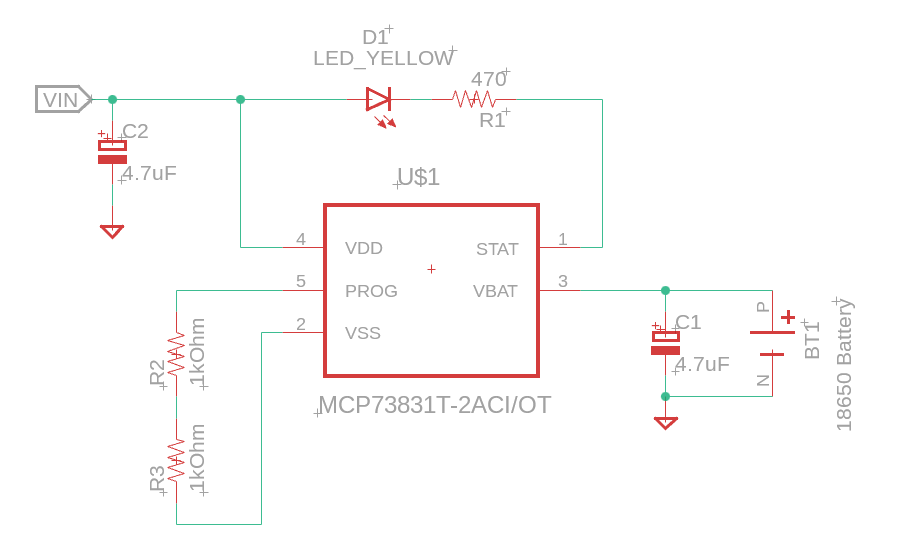
\includegraphics[width=0.75\linewidth]{Pictures/Circuito_cargador.png} 
  \caption{Circuito de carga MCP73831T-2ACI/OT configurado a 500 mA. }
  \label{fig:cargador}
\end{figure}

Es importante destacar que este cargador lineal está diseñado para una sola celda, por lo que se deberá implementar el circuito la misma cantidad de veces acorde a la cantidad de baterías.

Para realizar pruebas preliminares y verificar el rendimiento mediante prototipado rápido, hemos instalado en una placa de circuito impreso (PCB) el circuito cargador, para poder trabajar en conjunto con la PCB del arreglo de baterías (consultar Figuras \ref{fig:Chargerpistas} y \ref{fig:Charger3d}).

\begin{figure}
  \centering
  \begin{subfigure}{\linewidth}
    \centering
    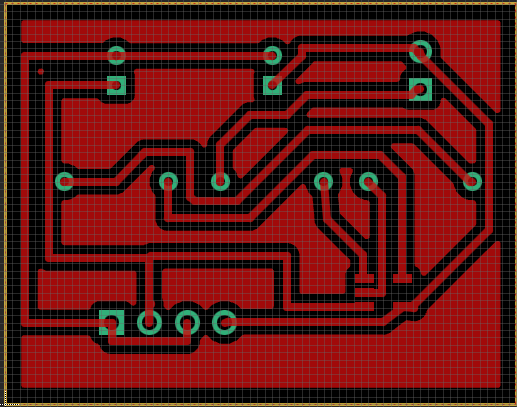
\includegraphics[width=0.4\linewidth]{Pictures/DesignPCBCharger.png}
    \caption{Diseño de pistas cargador MCP73831T-2ACI/OT}
    \label{fig:Chargerpistas}
  \end{subfigure}
  \begin{subfigure}{\linewidth}
    \centering
    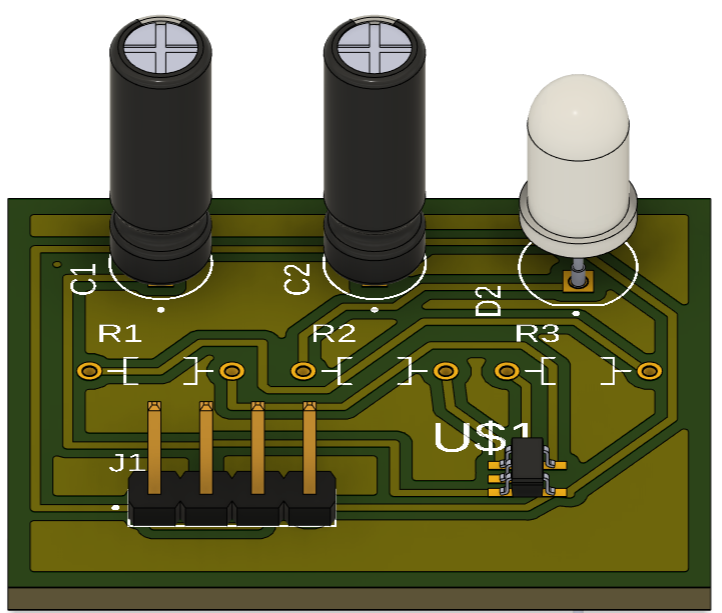
\includegraphics[width=0.4\linewidth]{Pictures/DesignPCBCharger3d.png}
    \caption{Vista 3D de PCB MCP73831T-2ACI/OT}
    \label{fig:Charger3d}
  \end{subfigure}
  \caption{Cargador de baterías}
  \label{fig:CHARGER-subfiguras}
\end{figure}

Como segunda alternativa, se consideran soluciones con cargadores comerciales. Un ejemplo de ello es el modelo D4 de Nitecore \cite{nitecore-d4-charger}, un sistema automatizado de carga de cuatro canales.

Finalmente, la elección entre el circuito de cargador lineal y el cargador comercial automatizado para esta etapa del EPS se tomará en función de evaluar el resto de los componentes, considerando criterios de complejidad y restricciones de espacio.


\section{Regulación de Voltaje}

Una de las etapas más críticas en el diseño, y que requiere una elección cuidadosa, es la conversión de voltaje. Esto se debe a factores esenciales, como la eficiencia de conversión y la compatibilidad con el banco de baterías. En el mercado, encontramos principalmente dos tipos de soluciones: reguladores de voltaje lineales y convertidores DC-DC.

En el diseño de circuitos electrónicos es bien conocido sobre la alta eficiencia de los convertidores DC-DC conmutados, pero los reguladores lineales siguen siendo la elección preferida en muchas aplicaciones. Comprender las razones detrás de esta preferencia ayudará a tomar decisiones acertadas e implementarlas de manera efectiva \cite{digikey-linear-regulators}.

\subsection{Reguladores lineales}

Los reguladores lineales presentan ventajas notables, como su simplicidad, costo asequible, necesidad reducida de componentes externos y ausencia de ruido por conmutación. Sin embargo, su principal desventaja es su baja eficiencia, la cual empeora a medida que aumenta la diferencia entre el voltaje de entrada y el voltaje regulado en la salida. Es crucial tener en cuenta que estos dispositivos no son capaces de aumentar el voltaje, lo que significa que, al utilizar un banco de baterías, es necesario configurarlo de manera que suministre un voltaje mínimo superior al voltaje requerido por el regulador. Además, es importante considerar que el voltaje de la batería no es constante y varía en función de su nivel de carga, generalmente oscilando entre 4.2 V y 2.5 V en el caso de baterías de iones de litio 18650, como las utilizadas en este trabajo. Esto podría dar lugar al inconveniente de no aprovechar toda la energía disponible debido a la falta de voltaje adecuado. A pesar de estas limitaciones, en aplicaciones específicas, los reguladores lineales pueden ser una elección adecuada (ver Tabla \ref{tab:caracteristicas_LDO}).


\subsection{Convertidores DC-DC}

Los reguladores conmutados son altamente eficientes y pueden elevar, reducir e invertir voltajes con facilidad. En muchos casos, es posible configurar un convertidor DC-DC en modo de elevación ('boost') o reducción de voltaje ('buck') de forma estática, lo cual es adecuado para aplicaciones con fuentes de voltaje DC constantes en el tiempo. Además, en el caso de aplicaciones que utilizan bancos de baterías, algunos modelos de convertidores DC-DC ofrecen la opción del modo buck-boost, que proporciona un voltaje de salida constante y programable. Este enfoque utiliza un esquema de control que permite una transición automática y suave entre los modos de boost, buck-boost y buck, lo que permite aprovechar al máximo la energía disponible en el rango de voltaje seguro de la batería.

Sin embargo, los reguladores conmutados también presentan algunas desventajas. En primer lugar, son componentes complejos, y su integración puede requerir un esfuerzo adicional de diseño. En segundo lugar, la alta integración puede aumentar los costos y el tamaño del chip. Por último, la conmutación a alta frecuencia tiende a generar ruido.

El rizado de voltaje y corriente en los filtros de entrada y salida, causado por la operación a alta frecuencia, puede ser un problema importante en un diseño con un regulador conmutado. Aunque estos problemas se pueden abordar, requieren tiempo y habilidad en el diseño (ver Tabla \ref{tab:caracteristicas_DC_DC}).



\begin{table}[h]
    \centering
    \caption{Características de regulador de voltaje lineal}
    \label{tab:caracteristicas_LDO}
    \begin{tabular}{ll}
        \toprule
        Característica & Regulador de voltaje lineal \\ 
        \midrule
        Función & Regulación descendente (buck) \\ 
        Eficiencia & Baja a media, alta si diferencia entre voltajes es pequeña \\ 
        Generación de calor & Alta si carga o diferencia de voltaje son altas \\ 
        Complejidad & Baja, regulador y condensadores \\ 
        Tamaño & Pequeño-mediano en portátiles \\ 
        Costo & Bajo \\ 
        Ruido & Bajo; mejor rechazo \\ 
        \bottomrule
    \end{tabular}
\end{table}

\begin{table}[h]
    \centering
    \caption{Características de convertidor DC-DC}
    \label{tab:caracteristicas_DC_DC}
    \begin{tabular}{ll}
        \toprule
        Característica & Convertidor DC-DC \\ 
        \midrule
        Función & Regulación elevador (boost), reductor (buck), inversor \\ 
        Eficiencia & Alta, excepto a corrientes muy bajas \\ 
        Calor & Baja, componentes fríos a <10W \\ 
        Complejidad & Media-alta: inductor, diodo, condensadores, FET en alta potencia \\ 
        Tamaño & Mayor que lineal a baja potencia, menor que lineal con disipador \\ 
        Costo & Medio-alto, debido a componentes externos \\ 
        Ruido & Medio-alto, ruido a frecuencia de conmutación \\ 
        \bottomrule
    \end{tabular}
\end{table}

\subsection{Análisis previo a implementación}

Centrándonos en la implementación, realizaremos una comparativa entre dos modelos comerciales. Por un lado, tenemos el convertidor de voltaje lineal LT1117 de Analog Devices (consultar Figura \ref{fig:LT1117_IC}), que es asequible y está respaldado por una documentación sólida \cite{analog_lt1117fd}. Por otro lado, evaluaremos el convertidor DC-DC MC34063A de Texas Instruments, que se destaca por su alta disponibilidad en el mercado internacional y su bajo costo \cite{ti_mc34063a} (ver Figura \ref{fig:MC34063_IC}).

\textbf{LT1117}

\begin{figure}[h]
  \centering
  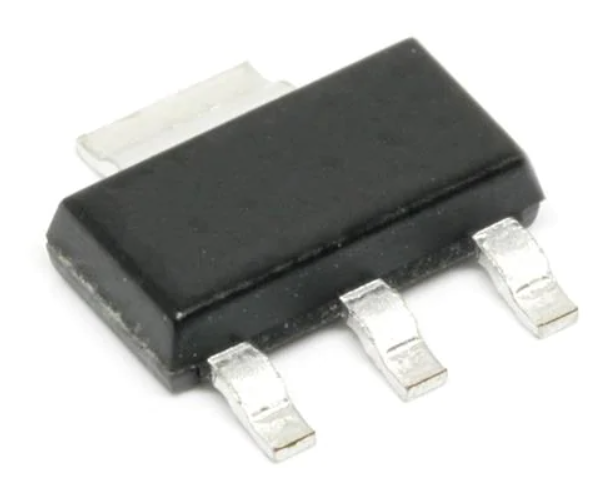
\includegraphics[width=0.20\linewidth]{Pictures/LT1117_AnalogD.png} 
  \caption{Circuito Integrado LT1117}
  \label{fig:LT1117_IC}
\end{figure}

La implementación del regulador lineal LT1117 es un proceso significativamente más simple. Es simplemente seguir el esquemático que se muestra en la Figura \ref{fig:Esquematico_LT1117_IC}.

\begin{figure}[h]
\centering
\includegraphics[width=0.42\linewidth]{Pictures/Esquemático LT1117_IC.png}
\caption{Esquemático del regulador lineal LT1117}
\label{fig:Esquematico_LT1117_IC}
\end{figure}


Para determinar los valores apropiados de resistencias, se utiliza la ecuación \ref{eq:tension_salida_LT1117}.

\begin{equation}\label{eq:tension_salida_LT1117}
V_{\text{out}} = 1.25 \, \text{V} \left(1 + \frac{R2}{R1}\right)
\end{equation}

Este enfoque simplificado facilita el diseño del regulador lineal LT1117. Ahora bien, para poder determinar la potencia disipada, Analog Devices en su hoja técnica brinda la ecuación \ref{eq:potencia_dissipada}.
\newpage
\begin{equation}
P_D = (V_{in} - V_{out}) \cdot I_{out}
\label{eq:potencia_dissipada}
\end{equation}


Donde:\\
$P_D$ es la potencia disipada.\\
$V_{in}$ es el voltaje de entrada.\\
$V_{out}$ es el voltaje de salida.\\
$I_{out}$ es la corriente de salida.

La eficiencia de un sistema (E) se define como la relación entre la potencia de salida ($P_{\text{out}}$) y la potencia de entrada ($P_{\text{in}}$), y se expresa en la ecuación \ref{eq:eficiencia}.

\begin{equation}
E = \frac{P_{\text{out}}}{P_{\text{in}}}
\label{eq:eficiencia}
\end{equation}

Donde, según la ecuación \ref{eq:potencia_dissipada}, la potencia de entrada ($P_{\text{in}}$) se calcula como:

\begin{equation}
P_{\text{in}} = (V_{\text{in}} - V_{\text{out}}) \cdot I_{\text{out}} + V_{\text{out}} \cdot I_{\text{out}}
\label{eq:eficiencia2}
\end{equation}

Y la potencia de salida ($P_{\text{out}}$) se calcula como:

\begin{equation}
P_{\text{out}} = V_{\text{out}} \cdot I_{\text{out}}
\label{eq:eficiencia3}
\end{equation}

Utilizando estas ecuaciones, podemos determinar la eficiencia porcentual de un regulador lineal como:

\begin{equation}
E (\%) = \frac{V_{\text{out}}}{V_{\text{in}}}\cdot 100\%.
\label{eq:eficiencia4}
\end{equation}

La eficiencia de la implementación de reguladores lineales se convierte en un tema preocupante cuando existe una diferencia significativa entre el voltaje de entrada y el de salida. \\\\Si consideramos las configuraciones previamente definidas (4s1p, 2s2p y 1s4p) para el banco de baterías, con voltajes nominales de entrada de 14.4 V, 7.2 V y 3.6 V respectivamente, podemos obtener resultados gráficos a partir de la ecuación \ref{eq:eficiencia4}, como se muestra en la Fig. \ref{fig:LDO_Efficiency}.

\newpage

\begin{figure}[h]
  \centering
  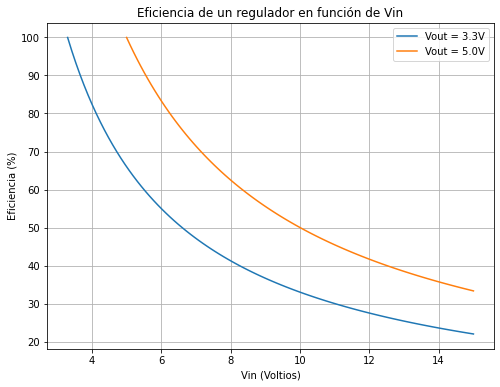
\includegraphics[width=0.8\linewidth]{Pictures/Grafica_Eficiencia_LDO.png} 
  \caption{Eficiencia del regulador LT1117 en función del voltaje de entrada ($V_{in}$)}
  \label{fig:LDO_Efficiency}
\end{figure}

Como resultado del análisis de la gráfica y considerando el contexto de diseño en el que se utilizaría el regulador de voltaje lineal LT1117, se concluye que su implementación no es conveniente. En el caso de la configuración 4s1p, la eficiencia es notablemente baja, siendo inferior al 35\% tanto para el bus de 3.3 V como para el de 5.0 V. Aunque la situación mejora ligeramente en la configuración 2s2p donde el vin es de 7.2 V, la eficiencia aún no alcanza ni siquiera el 70\%.

Finalmente, para el arreglo 1s4p donde el voltaje de entrada inicial sería 3.6 V se presenta un inconveniente inherente a los reguladores lineales, ya que no es posible construir un elevador de voltaje ('boost') con este dispositivo. Esto significa que no se podría obtener un bus de 5.0 V. Para el voltaje de 3.3 V, según la hoja de datos del fabricante \cite{analog_lt1117fd}, el voltaje de entrada mínimo necesario para regular y llevarlo a 3.3 V debe ser al menos de 5.0 V. \\\\Además, en el bus de 3.3 V precisamente se presenta un escenario aún más complejo, nos encontramos en una situación en la que el voltaje de la batería disminuiría hasta un valor de 2.5 V, lo que requeriría nuevamente una configuración 'boost'. Por lo tanto, debido a estas limitaciones y desafíos técnicos, se descarta el uso de reguladores lineales para esta aplicación.
\newpage

\textbf{MC34063A}

\begin{figure}[h]
  \centering
  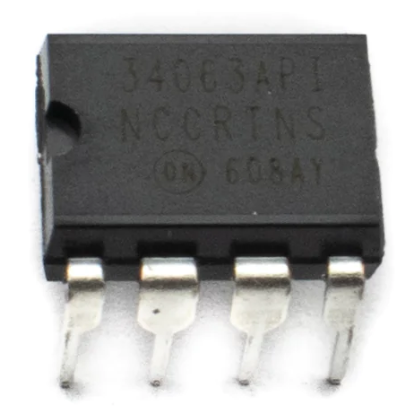
\includegraphics[width=0.25\linewidth]{Pictures/MC34063_IC.png} 
  \caption{Circuito Integrado MC34063A}
  \label{fig:MC34063_IC}
\end{figure}

Para la implementación del convertidor DC-DC MC34063, se emplean fórmulas esenciales proporcionadas por el fabricante y resumidas en la Tabla \ref{tab:forms_MC34063A} \cite{ti_mc34063a}. Adicionalmente, se utiliza una herramienta calculadora desarrollada por la comunidad de electrónicos para agilizar el proceso de diseño \cite{nomad_ee_mc34063a}. En cuanto al esquemático, se presenta la configuración Boost en la Figura \ref{fig:BoostMC} y la configuración Buck en la Figura \ref{fig:BuckMC}. La evaluación de la eficiencia se basa en tablas de referencia proporcionadas por el fabricante.

\begin{figure}[h]
  \centering
  \begin{subfigure}{0.4\linewidth}
    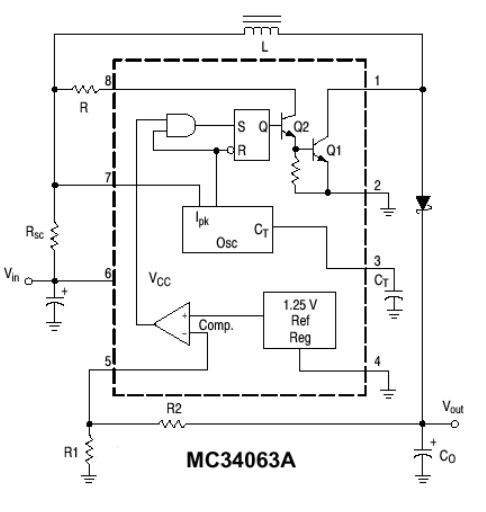
\includegraphics[width=\textwidth]{Pictures/Esquematico_Boost_Converter.png}
    \caption{MC34063A Configuración Boost}
    \label{fig:BoostMC}
  \end{subfigure}
  \begin{subfigure}{0.42\linewidth}
    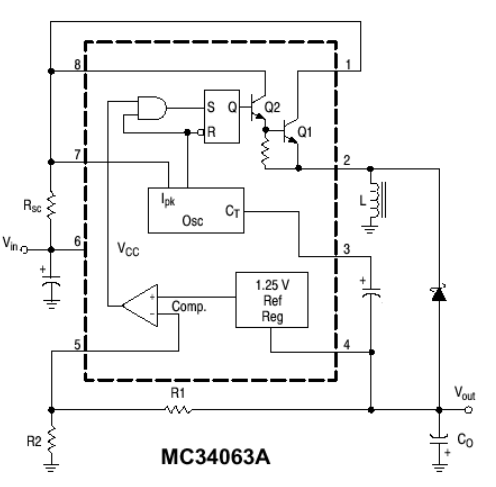
\includegraphics[width=\textwidth]{Pictures/Esquematico_Buck_Converter.png}
    \caption{MC34063A Configuración Buck}
    \label{fig:BuckMC}
  \end{subfigure}
  \caption{Configuraciones MC34063A}
\end{figure}

\begin{table}[!ht]
    \centering
    \renewcommand{\arraystretch}{2} % Espacio entre filas
    \begin{adjustbox}{max width=\textwidth}
        \begin{tabular}{ccc}
            \hline
            \makecell{Cálculo} & \makecell{Step-Up} & \makecell{Step-Down} \\
            \hline
            \makecell{$\frac{t_{on}}{t_{off}}$} & \makecell{$\frac{{V_{out} + V_F + V_{in(min)}}}{V_{in(min)}-V_{sat}}$} & \makecell{$\frac{V_{out} + V_F}{V_{in(min)}-V_{sat}-V_{out}}$} \\
            \hline
            \makecell{$t_{on}+{t_{off}}$} & \makecell{$\frac{1}{f}$} & \makecell{$\frac{1}{f}$} \\
            \hline
            \makecell{$t_{off}$} & \makecell{$\frac{t_{on}+t_{off}}{\frac{t_{on}}{t_{off}}+1}$} & \makecell{$\frac{t_{on}+t_{off}}{\frac{t_{on}}{t_{off}}+1}$} \\
            \hline
            \makecell{$t_{on}$}  & \makecell{$(t_{on}+{t_{off}})-{t_{off}}$} & \makecell{$(t_{on}+{t_{off}})-{t_{off}}$} \\
            \hline
            \makecell{$C_T$} & \makecell{$4.0x10^{-5}t_{on}$} & \makecell{$4.0x10^{-5}t_{on}$} \\
            \hline
            \makecell{$I_{pk(switch)}$} & \makecell{$2I_{out(max)}(\frac{t_{on}}{t_{off}}+1)$} & \makecell{$2I_{out(max)}$} \\
            \hline
            \makecell{$R_{sc}$} & \makecell{$\frac{0.3}{I_{pk(switch)}}$} & \makecell{$\frac{0.3}{I_{pk(switch)}}$} \\
            \hline
            \makecell{$L_(min)$} & \makecell{$(\frac{(V_{in(min)}-V_{sat})}{I_{pk(switch)}})t_{on(max)}$} & \makecell{$(\frac{(V_{in(min)}-V_{sat})}{I_{pk(switch)}})t_{on(max)}$} \\
            \hline
            \makecell{$C_O$} & \makecell{$9\frac{I_{out}I_{on}}{V_{ripple(pp)}}$} & \makecell{$\frac{I_{pk(switch)}(t_{on} + t_{off})}{8V_{ripple(pp)}}$} \\
            \hline
        \end{tabular}
    \end{adjustbox}
    \caption{Fórmulas de diseño para MC34063A}
    \label{tab:forms_MC34063A}
\end{table}

Un aspecto importante resaltado en la Tabla \ref{tab:forms_MC34063A} es el cálculo de la inductancia. El fabricante especifica un valor mínimo, lo que significa que al diseñar el circuito, existe flexibilidad para realizar ajustes finos según los resultados en la señal de salida o la disponibilidad de valores comerciales. Tanto el inductor como el condensador 'Co' forman un filtro pasabajos de segundo orden que desempeña un papel crucial en el convertidor DC-DC al reducir los sobreimpulsos antes de alcanzar el valor de estado estable.

Al igual que con el regulador de voltaje lineal LT1117, con el convertidor DC-DC evaluaremos el rendimiento con las configuraciones del banco de baterías 4s1p, 2s2p y 1s4p, previamente desarrolladas en las  \ref{fig:powerbank}, \ref{fig:powerbank2} y \ref{fig:powerbank3}.

Previo a desarrollar las simulaciones debemos recordar que en el capítulo de Requerimientos se realizó un presupuesto energético para cubrir la demanda de los subsistemas electrónicos de la misión StratoBalloon en Tabla \ref{tab:cuadro-cargas1} y \ref{tab:cuadro-cargas2}. 

En el presupuesto energético preliminar, no se consideraron las pérdidas asociadas a esta etapa de conversión de voltaje DC-DC, ni tampoco el autoconsumo de otros componentes relacionados con el Sistema de energía (EPS). Por lo tanto, al finalizar este capítulo, se llevará a cabo una revisión tomando estas consideraciones. Esto permitirá evaluar si el dimensionamiento del banco de baterías es adecuado. Dicho esto, iniciamos con la evaluación del convertidor para cada arreglo.

\newpage

%ARREGLO DE BATERÍAS 4S1P

\subsection{Arreglo de baterías 4s1p}

Como punto de partida consideramos el arreglo 4s1p. Para este arreglo, se toman en cuenta los valores detallados en la Tabla \ref{tab:valores_33_4s1p}

\begin{table*}[h]
    \centering
    \begin{tabular}{p{0.25\linewidth}p{0.1\linewidth}p{0.25\linewidth}p{0.1\linewidth}}
    \hline
    \textbf{Entradas} & \textbf{Valor} & \textbf{Salidas} & \textbf{Valor} \\ \hline
    Vin (min)[V] & 10.0 & Ct [pF] & 157 \\
    Vout [V] & 3.3 & Ipk [mA] & 1500 \\
    Iout [mA] & 750 & Rsc [Ohm] & 0.2 \\
    V ripple pp [mV] & 10 & Lmin [uH] & 15 \\
    Fmin [kHz] & 100 & Co [uF] & 188 \\
    ~ & ~ & R1 [kohm] & 11 \\
    ~ & ~ & R2 [kohm] & 18 \\ \hline
    \end{tabular}
\caption{Valores para convertidor DC-DC MC34063A, bus 3.3 V a 750 mA.}
\label{tab:valores_33_4s1p}
\end{table*}

Como resultado obtenemos la señal de voltaje de salida para el arreglo de baterías 4s1p a máxima carga en Fig. \ref{fig:4s1p_33v_2dcdcconverters_Max} y para mínima carga en Fig. \ref{fig:4s1p_33v_2dcdcconverters_min}.

\begin{figure}[h]
  \centering
  \begin{subfigure}{0.48\linewidth}
    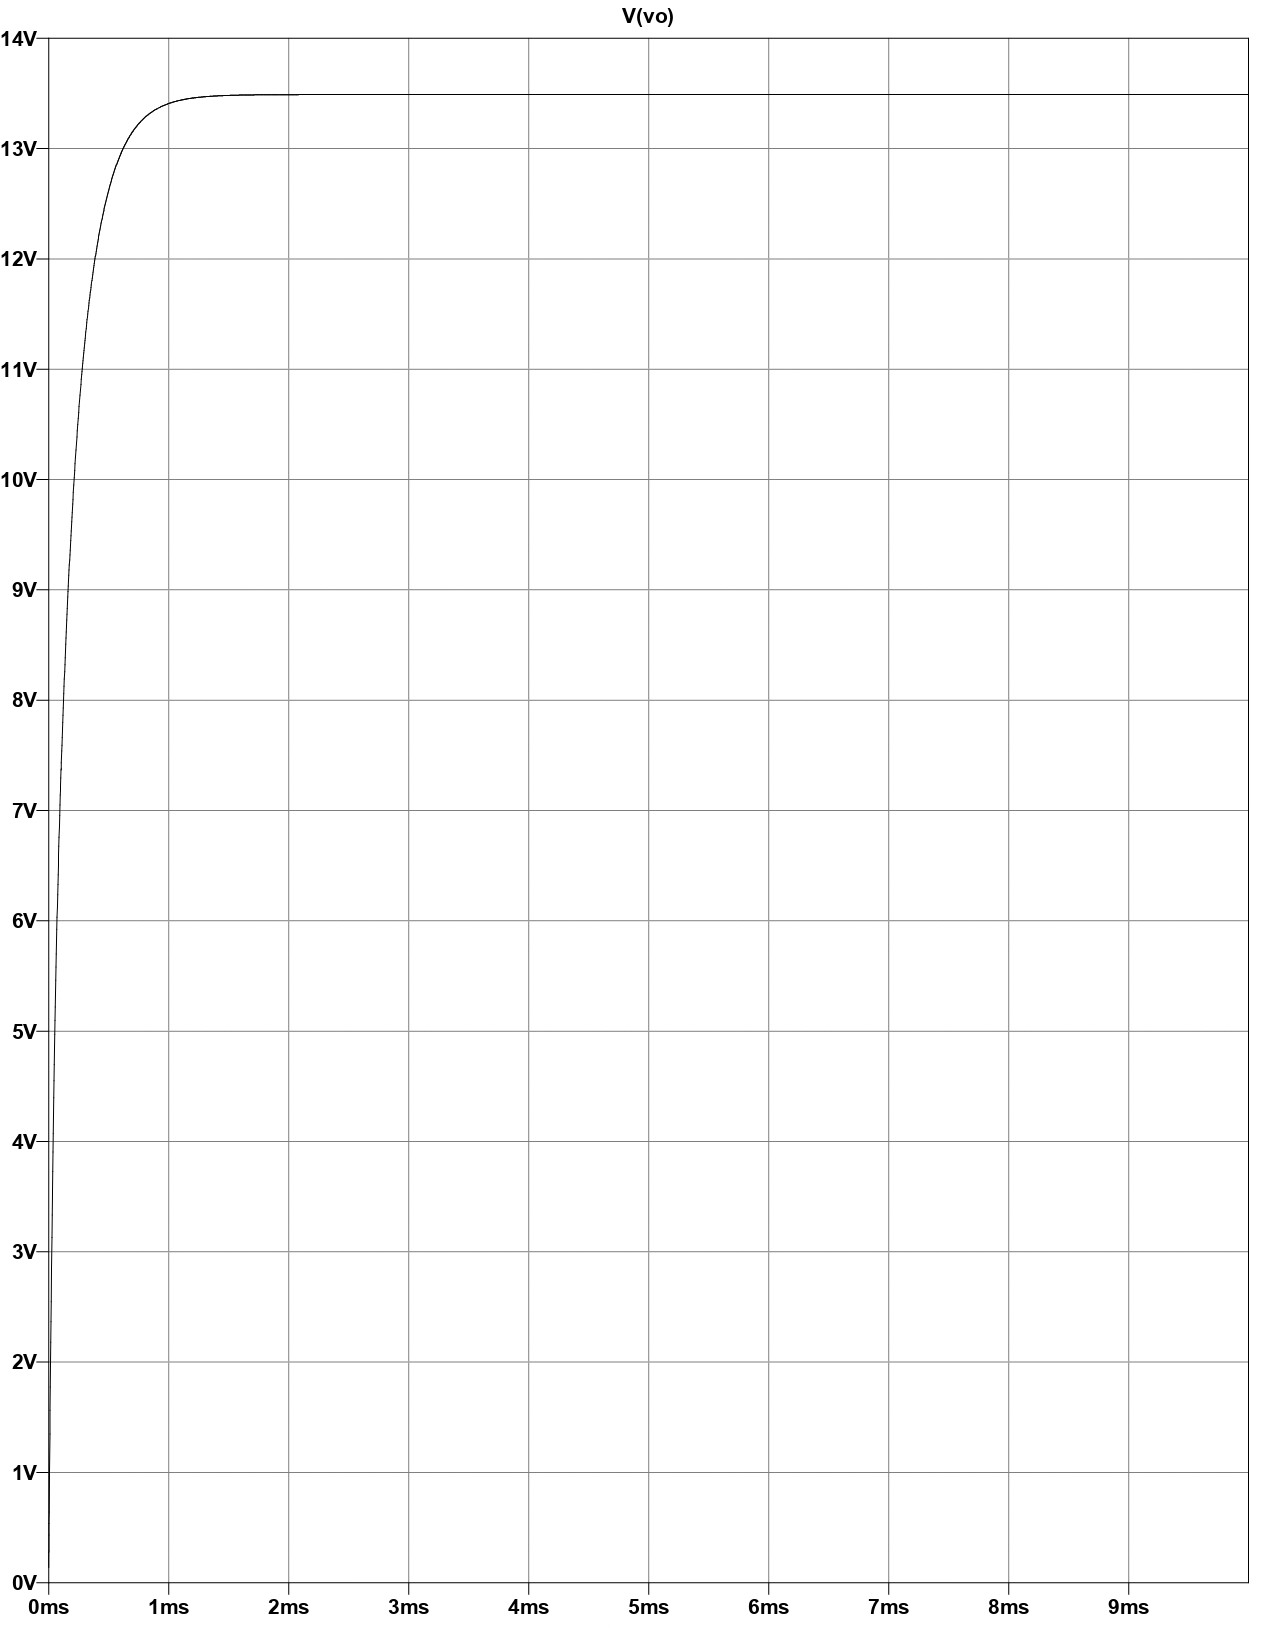
\includegraphics[width=\textwidth]{Pictures/Convertidor DC-DC MC34063A, bus 3.3 v a 750 mA_page-0001.jpg}
    \caption{Salida de voltaje a 3.3 voltios. Vin máximo (16.8 V)}
    \label{fig:4s1p_33v_2dcdcconverters_Max}
  \end{subfigure}
  \hfill
  \begin{subfigure}{0.48\linewidth}
    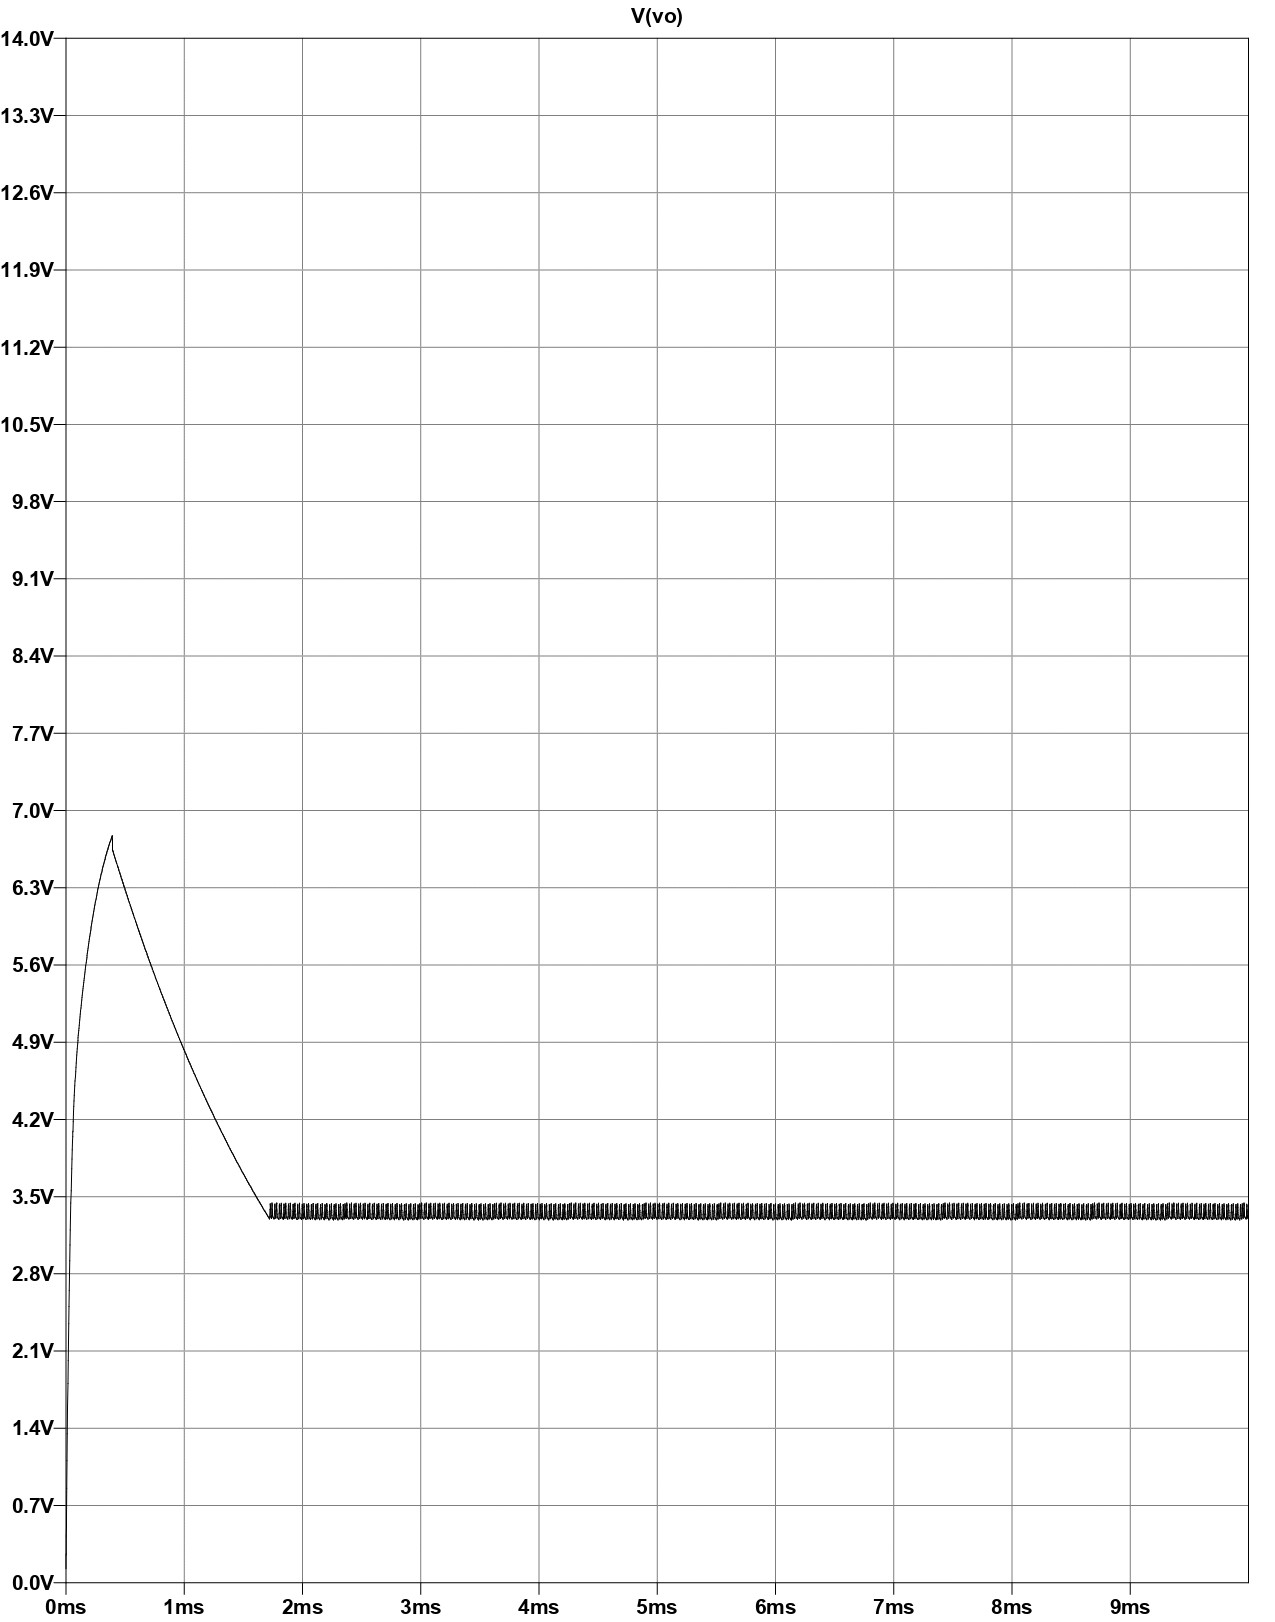
\includegraphics[width=\textwidth]{Pictures/Convertidor DC-DC MC34063A, bus 3.3 v a 750 mA_page-0001 Min.jpg}
    \caption{Salida de voltaje a 3.3 voltios. Vin mínimo. (10.0 V)}
    \label{fig:4s1p_33v_2dcdcconverters_min}
  \end{subfigure}
  \caption{Convertidor DC-DC MC34063A, arreglo 4s1p, bus de 3.3 V a 750 mA.}
  \label{fig:ConveridorDCDC_4S1P_33V}
\end{figure}

En el primer escenario (Fig. \ref{fig:4s1p_33v_2dcdcconverters_Max}), con las baterías completamente cargadas, observamos que el convertidor DC-DC no alcanza el valor de voltaje regulado.

En el escenario opuesto (Fig. \ref{fig:ConveridorDCDC_4S1P_33V}), con las baterías descargadas al mínimo, logramos alcanzar el valor deseado en estado estable. Sin embargo, se produce un sobreimpulso que alcanza hasta 6.3V, lo que representa un riesgo para los dispositivos electrónicos alimentados. La estabilización en 3.3V en este caso requiere aproximadamente 1.8 milisegundos. Por lo tanto, será necesario realizar un ajuste en el valor de la inductancia del circuito LC del convertidor.

Al ajustar los valores de la inductancia mínima a 30uH, obtenemos los resultados de la Fig. \ref{fig:ConveridorDCDC_4S1P_33V_ajustada}


\begin{figure}[h]
  \centering
  \begin{subfigure}{0.48\linewidth}
    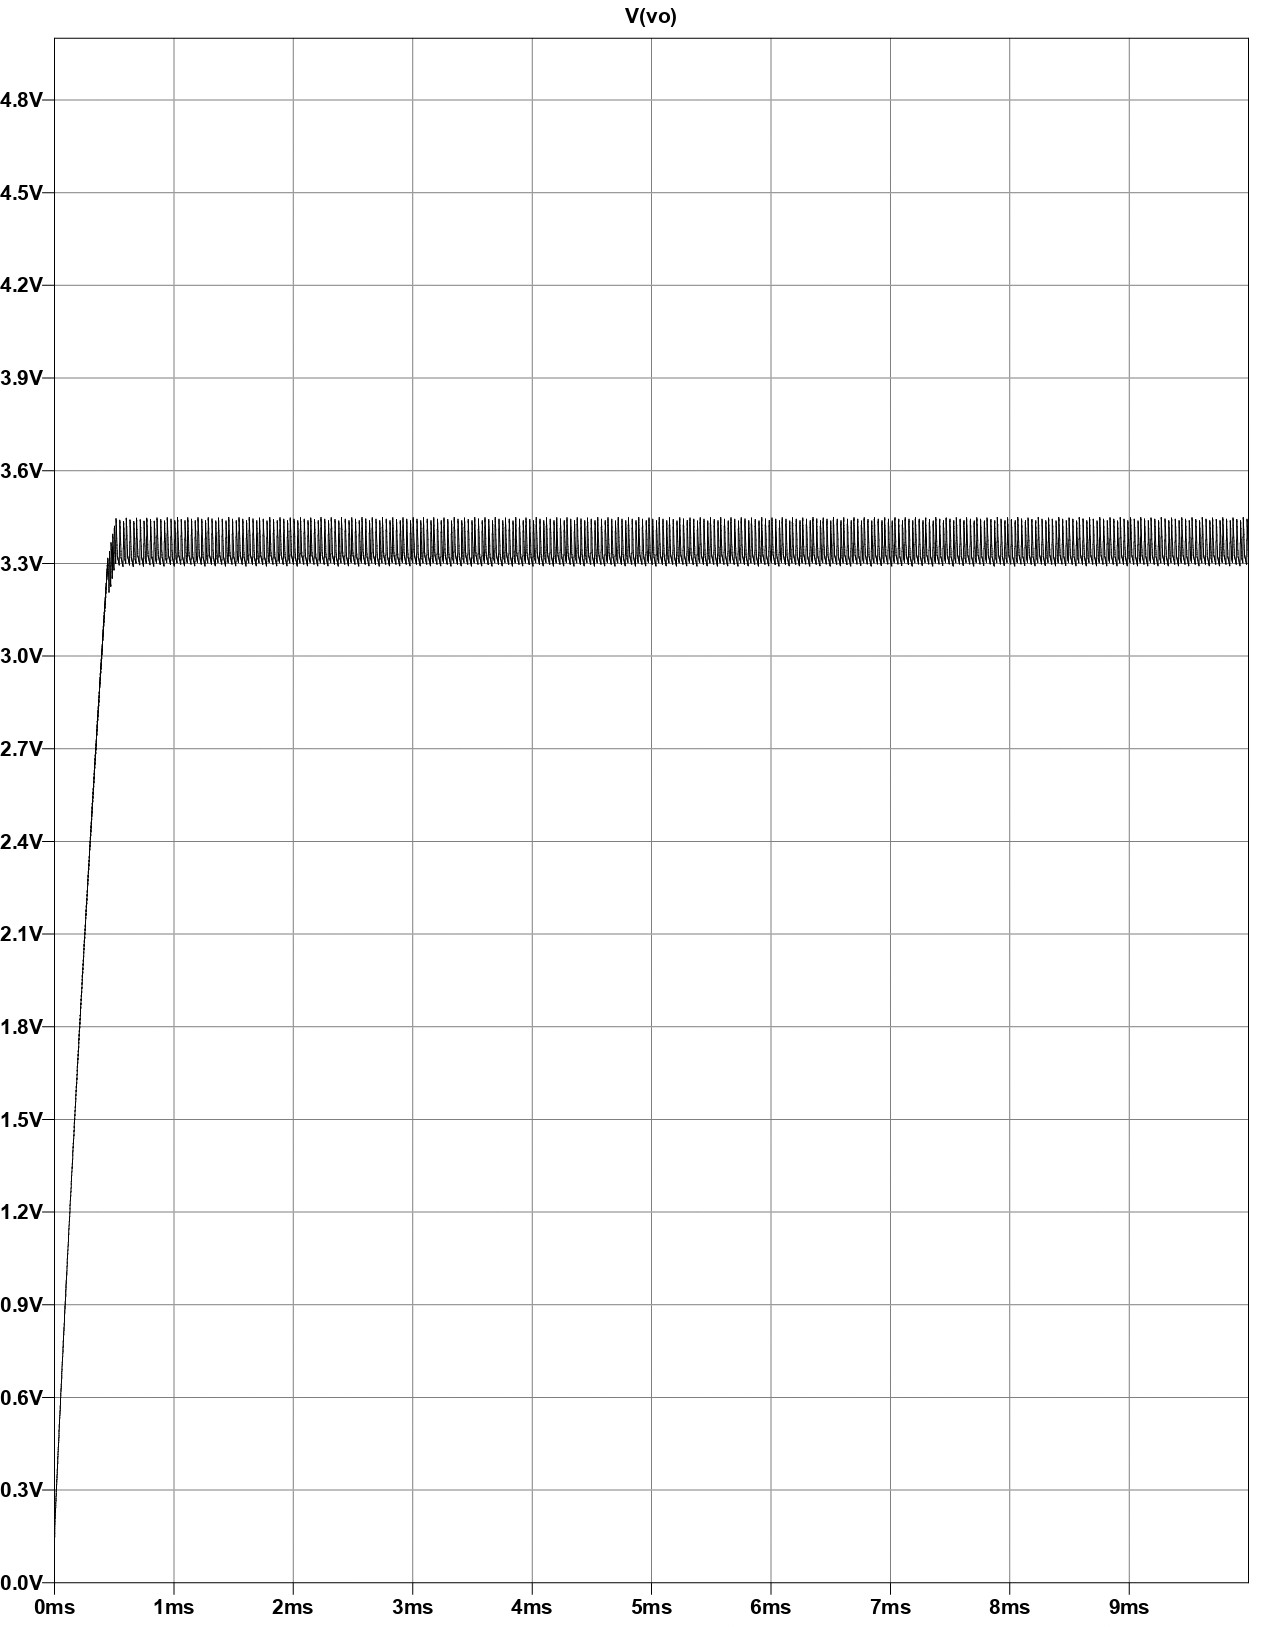
\includegraphics[width=\textwidth]{Pictures/Ajustada1_Max.jpg}
    \caption{Salida de voltaje a 3.3 voltios. Vin máximo (16.8 V). Inductancia ajustada a 30 uH.}
    \label{fig:4s1p_33v_2dcdcconverters_Max2}
  \end{subfigure}
  \hfill
  \begin{subfigure}{0.48\linewidth}
    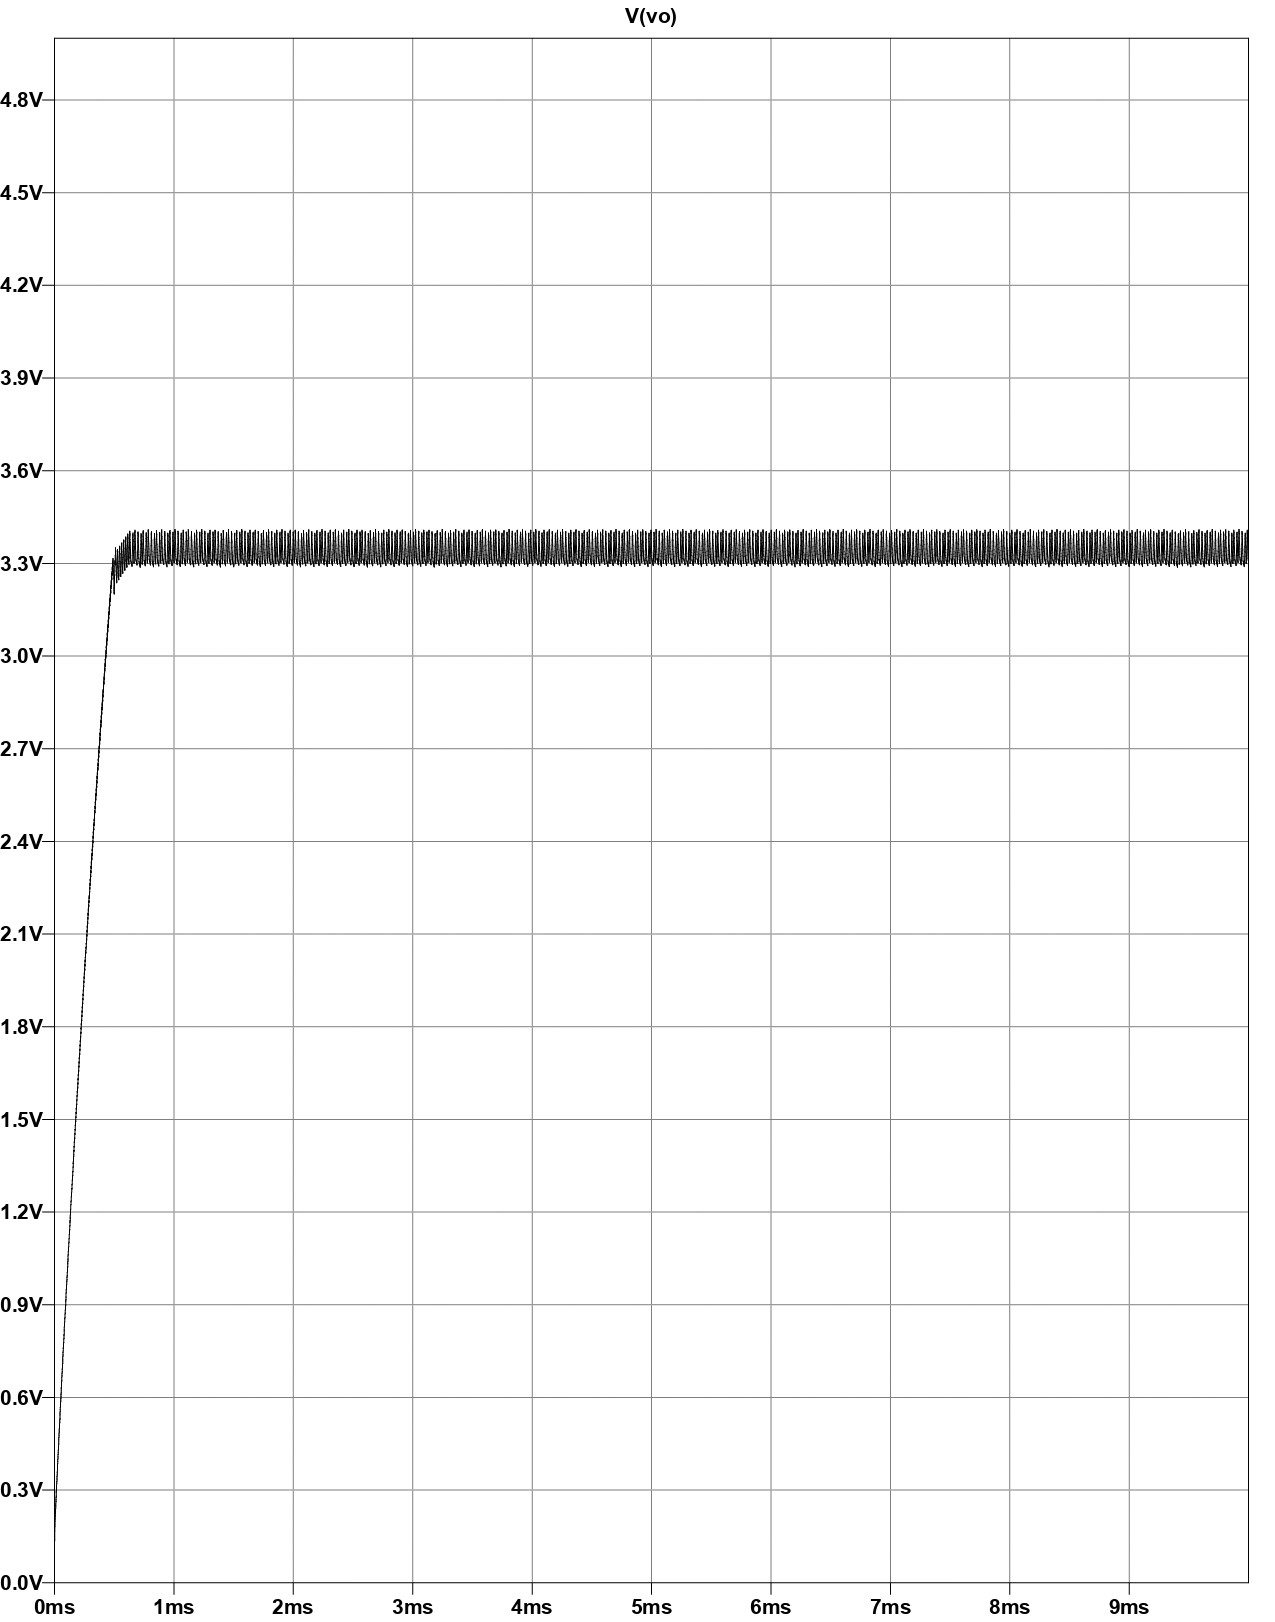
\includegraphics[width=\textwidth]{Pictures/Ajustada1_Min.jpg}
    \caption{Salida de voltaje a 3.3 voltios. Vin mínimo. (10.0 V). Inductancia ajustada a 30 uH.}
    \label{fig:4s1p_33v_2dcdcconverters_min2}
  \end{subfigure}
  \caption{Convertidor DC-DC MC34063A, arreglo 4s1p, bus de 3.3 V a 750 mA. Inductancia ajustada a 30 uH.}
  \label{fig:ConveridorDCDC_4S1P_33V_ajustada}
\end{figure}

Podemos observar que en ambos casos, los resultados son satisfactorios para alimentar las cargas. Tanto el valor pico a pico como el sobreimpulso se encuentran en niveles despreciables, lo que representa un resultado satisfactorio tanto en el caso del banco de baterías a máxima carga (ver Fig. \ref{fig:4s1p_33v_2dcdcconverters_Max2}) como en el caso de mínima carga (ver Fig. \ref{fig:ConveridorDCDC_4S1P_33V_ajustada}).

\newpage

% PARA EL BUS DE 5.0 VOLTIOS ************

Siguiendo un procedimiento similar, empleando los datos de la Tabla \ref{tab:valores_50_4s1p}, obtenemos los resultados para el voltaje máximo del banco de baterías en configuración 4s1p en Fig. \ref{fig:4s1p_50v_2dcdcconverters_Max} y el mínimo en Fig. \ref{fig:4s1p_50v_2dcdcconverters_min}.

\begin{table*}[h]
    \centering
    \begin{tabular}{p{0.25\linewidth}p{0.1\linewidth}p{0.25\linewidth}p{0.1\linewidth}}
    \hline
    \textbf{Entradas} & \textbf{Valor} & \textbf{Salidas} & \textbf{Valor} \\ \hline
    Vin (min)[V] & 10.0 & Ct [pF] & 230 \\
    Vout [V] & 5.0 & Ipk [mA] & 1500 \\
    Iout [mA] & 750 & Rsc [Ohm] & 0.2 \\
    V ripple pp [mV] & 10 & Lmin [uH] & 15 \\
    Fmin [kHz] & 100 & Co [uF] & 188 \\
    ~ & ~ & R1 [kohm] & 1 \\
    ~ & ~ & R2 [kohm] & 3 \\ \hline
    \end{tabular}
\caption{Valores para convertidor DC-DC MC34063A, arreglo 4s1p, bus 5.0 V a 750 mA.}
\label{tab:valores_50_4s1p}
\end{table*}


\begin{figure}[h]
  \centering
  \begin{subfigure}{0.48\linewidth}
    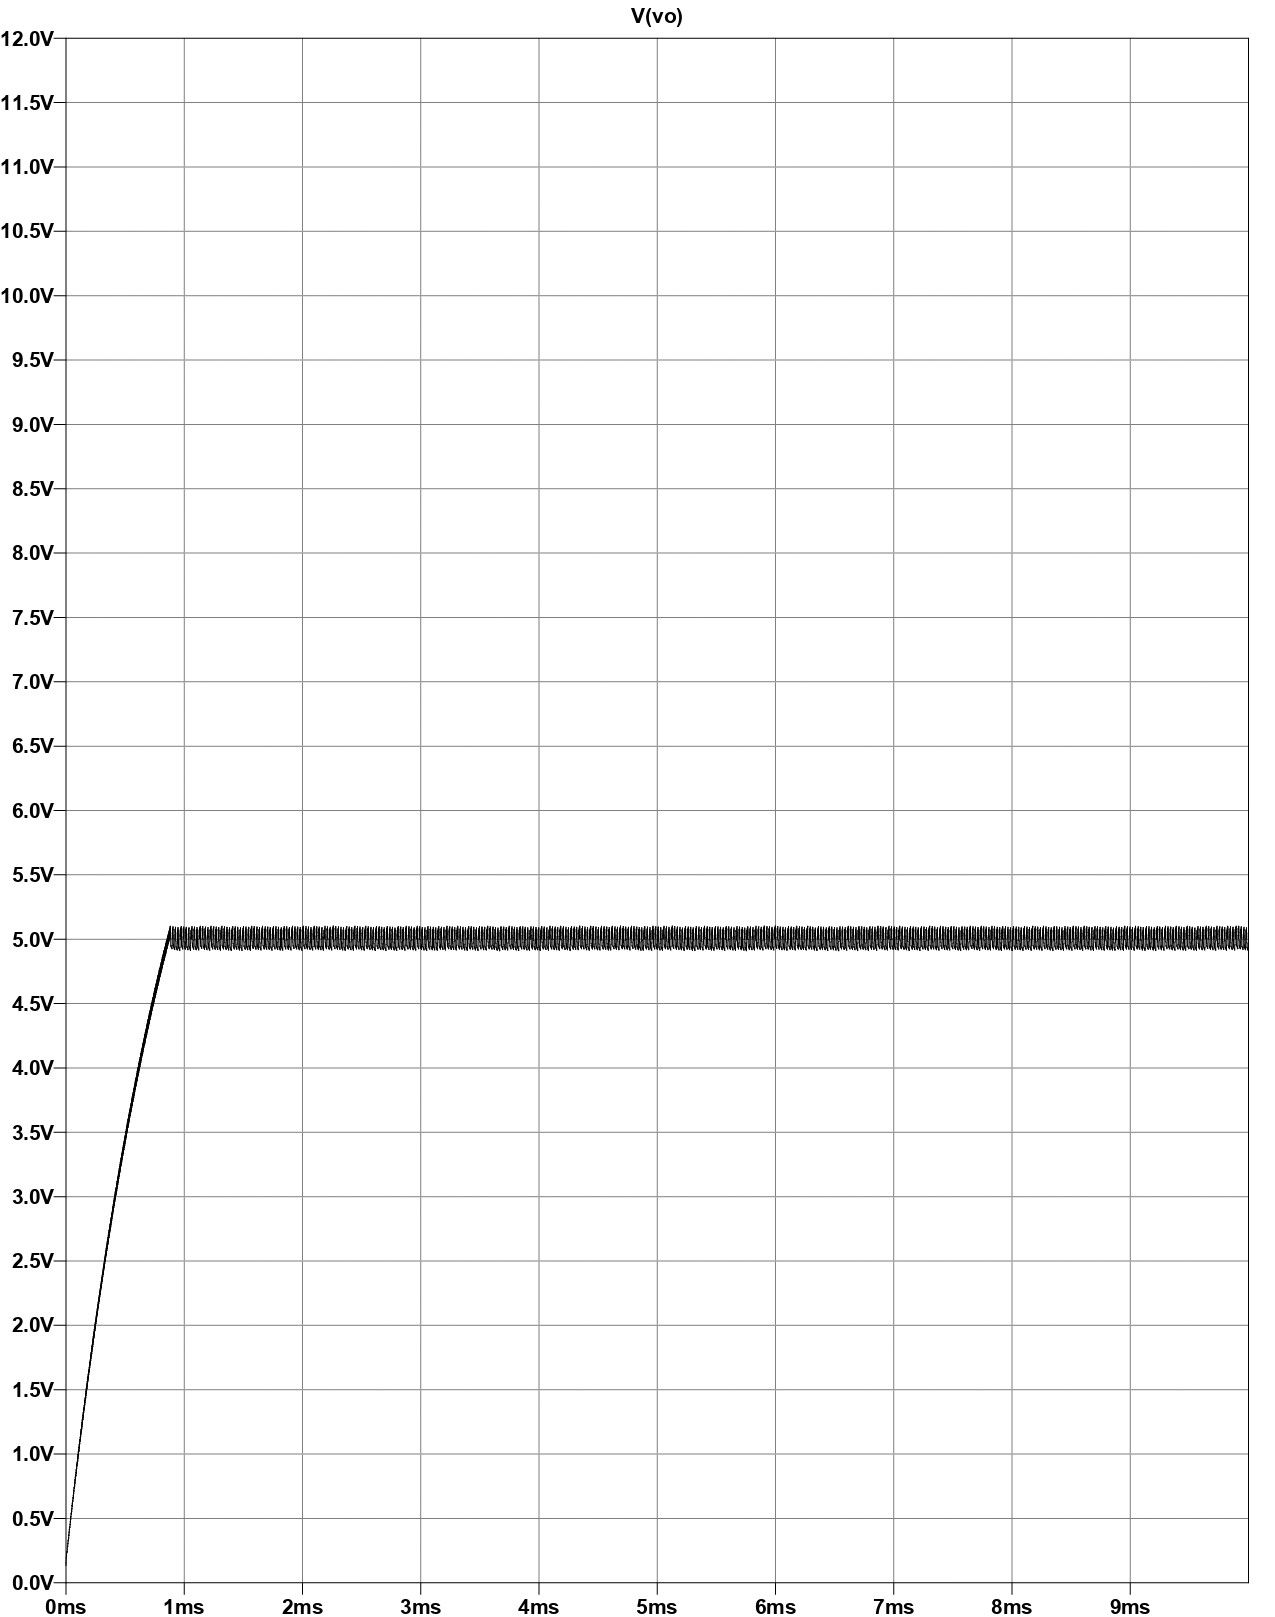
\includegraphics[width=\textwidth]{Pictures/Convertidor DC-DC MC34063A, bus 5.0 v a 750 mA_page-0001 Max.jpg}
    \caption{Salida de voltaje a 5.0 voltios. Vin máximo (16.8 V)}
    \label{fig:4s1p_50v_2dcdcconverters_Max}
  \end{subfigure}
  \hfill
  \begin{subfigure}{0.48\linewidth}
    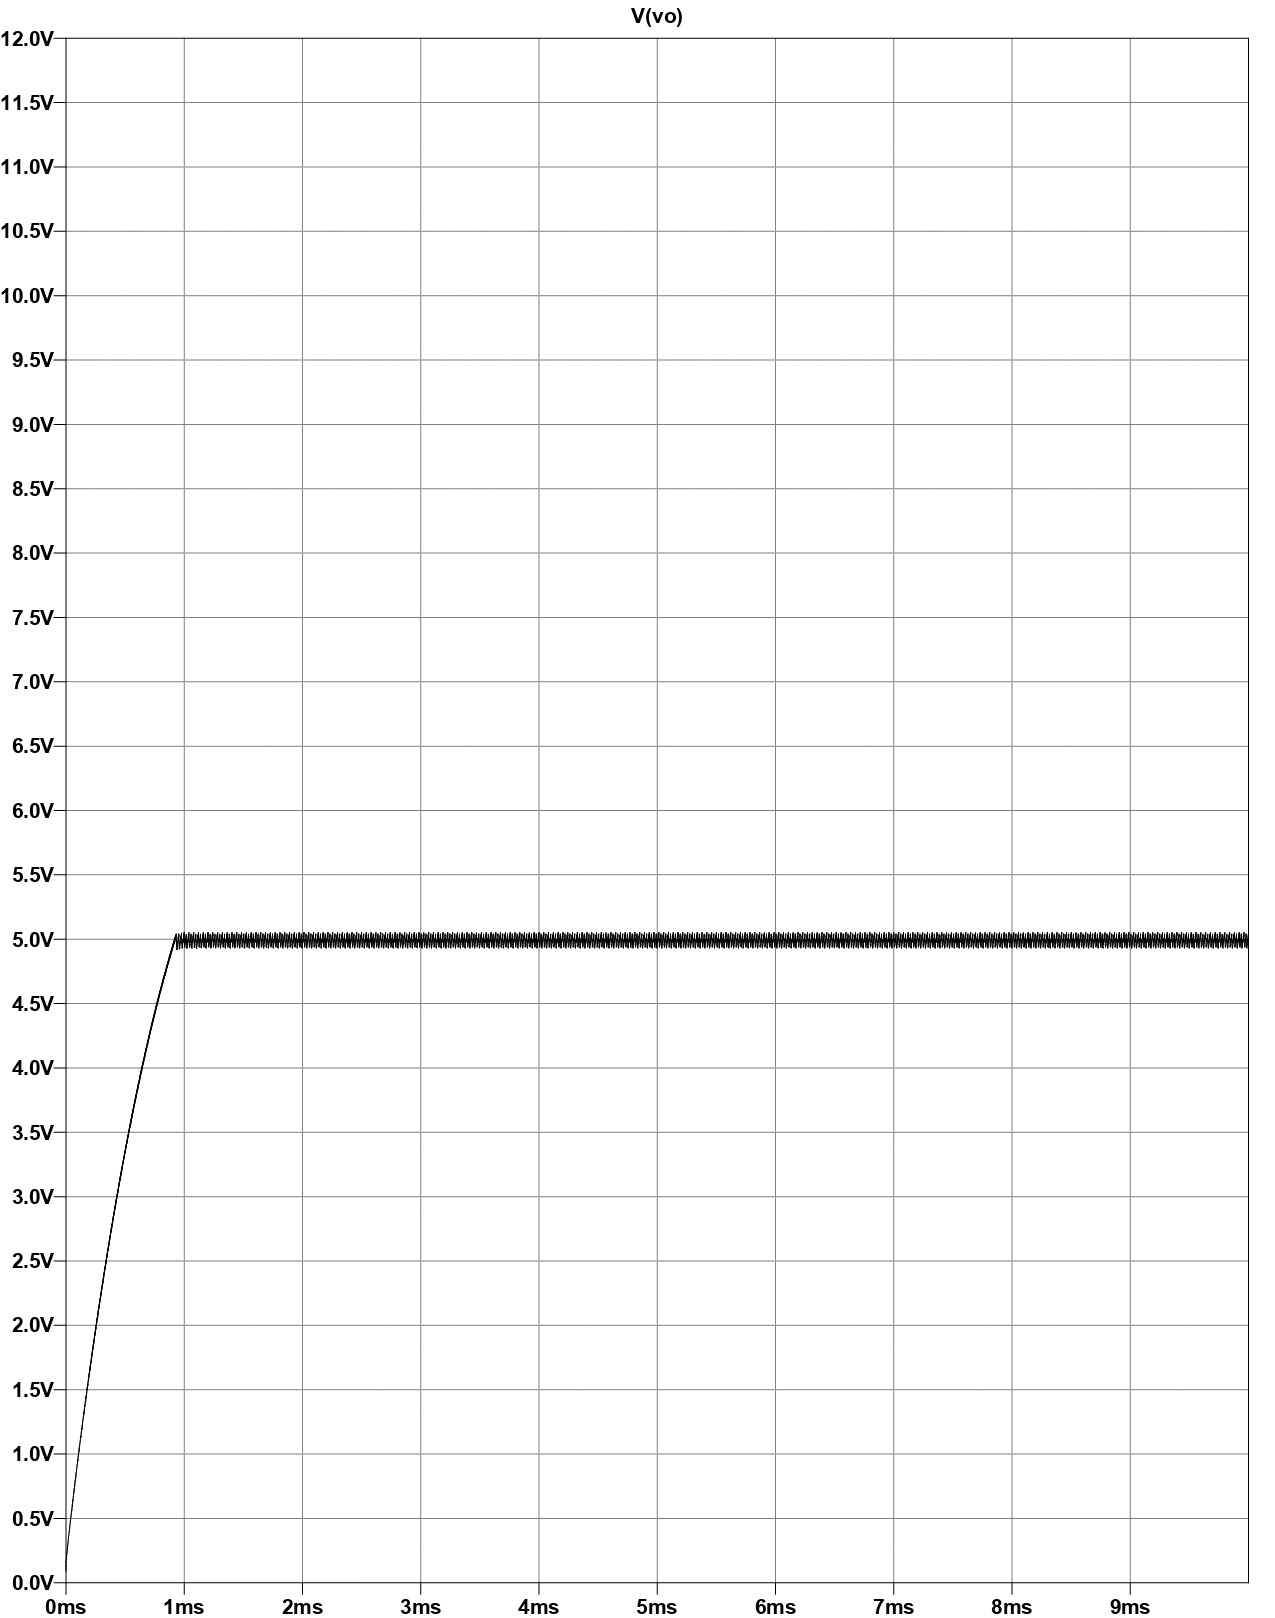
\includegraphics[width=\textwidth]{Pictures/Convertidor DC-DC MC34063A, bus 5.0 v a 750 mA_page-0001 Min.jpg}
    \caption{Salida de voltaje a 5.0 voltios. Vin mínimo. (10.0 V)}
    \label{fig:4s1p_50v_2dcdcconverters_min}
  \end{subfigure}
  \caption{Convertidor DC-DC MC34063A, arreglo 4s1p, bus de 5.0 V a 750 mA.}
\end{figure}

Podemos observar que en ambos casos, los resultados son satisfactorios para alimentar las cargas. Tanto el valor pico a pico como el sobreimpulso se encuentran en niveles despreciables, lo que representa un resultado satisfactorio sin requerir el ajuste de la inductancia del filtro pasabajos.




% ARREGLO 2S2P
\subsection{Arreglo de baterías 2s2p}
Como segundo arreglo del banco de baterías consideramos la configuración 2s2p. Empleamos los cálculos de la Fig. \ref{tab:valores_33_2s2p} y como resultado se obtiene la Fig. \ref{fig:2s2p_33v_2dcdcconverters_Max} para un banco de baterías con carga máxima y la Fig. \ref{fig:2s2p_33v_2dcdcconverters_min} para carga al mínimo.

% PARA EL BUS DE 3.3 VOLTIOS ************

\begin{table*}[h]
    \centering
    \begin{tabular}{p{0.25\linewidth}p{0.1\linewidth}p{0.25\linewidth}p{0.1\linewidth}}
    \hline
    \textbf{Entradas} & \textbf{Valor} & \textbf{Salidas} & \textbf{Valor} \\ \hline
    Vin (min)[V] & 5.0 & Ct [pF] & 336 \\
    Vout [V] & 3.3 & Ipk [mA] & 1500 \\
    Iout [mA] & 750 & Rsc [Ohm] & 0.2 \\
    V ripple pp [mV] & 10 & Lmin [uH] & 4 \\
    Fmin [kHz] & 100 & Co [uF] & 188 \\
    ~ & ~ & R1 [kohm] & 11 \\
    ~ & ~ & R2 [kohm] & 18 \\ \hline
    \end{tabular}
\caption{Valores para convertidor DC-DC MC34063A, arreglo 2s2p, bus 3.3 V a 750 mA.}
\label{tab:valores_33_2s2p}
\end{table*}


\begin{figure}[h]
  \centering
  \begin{subfigure}{0.48\linewidth}
    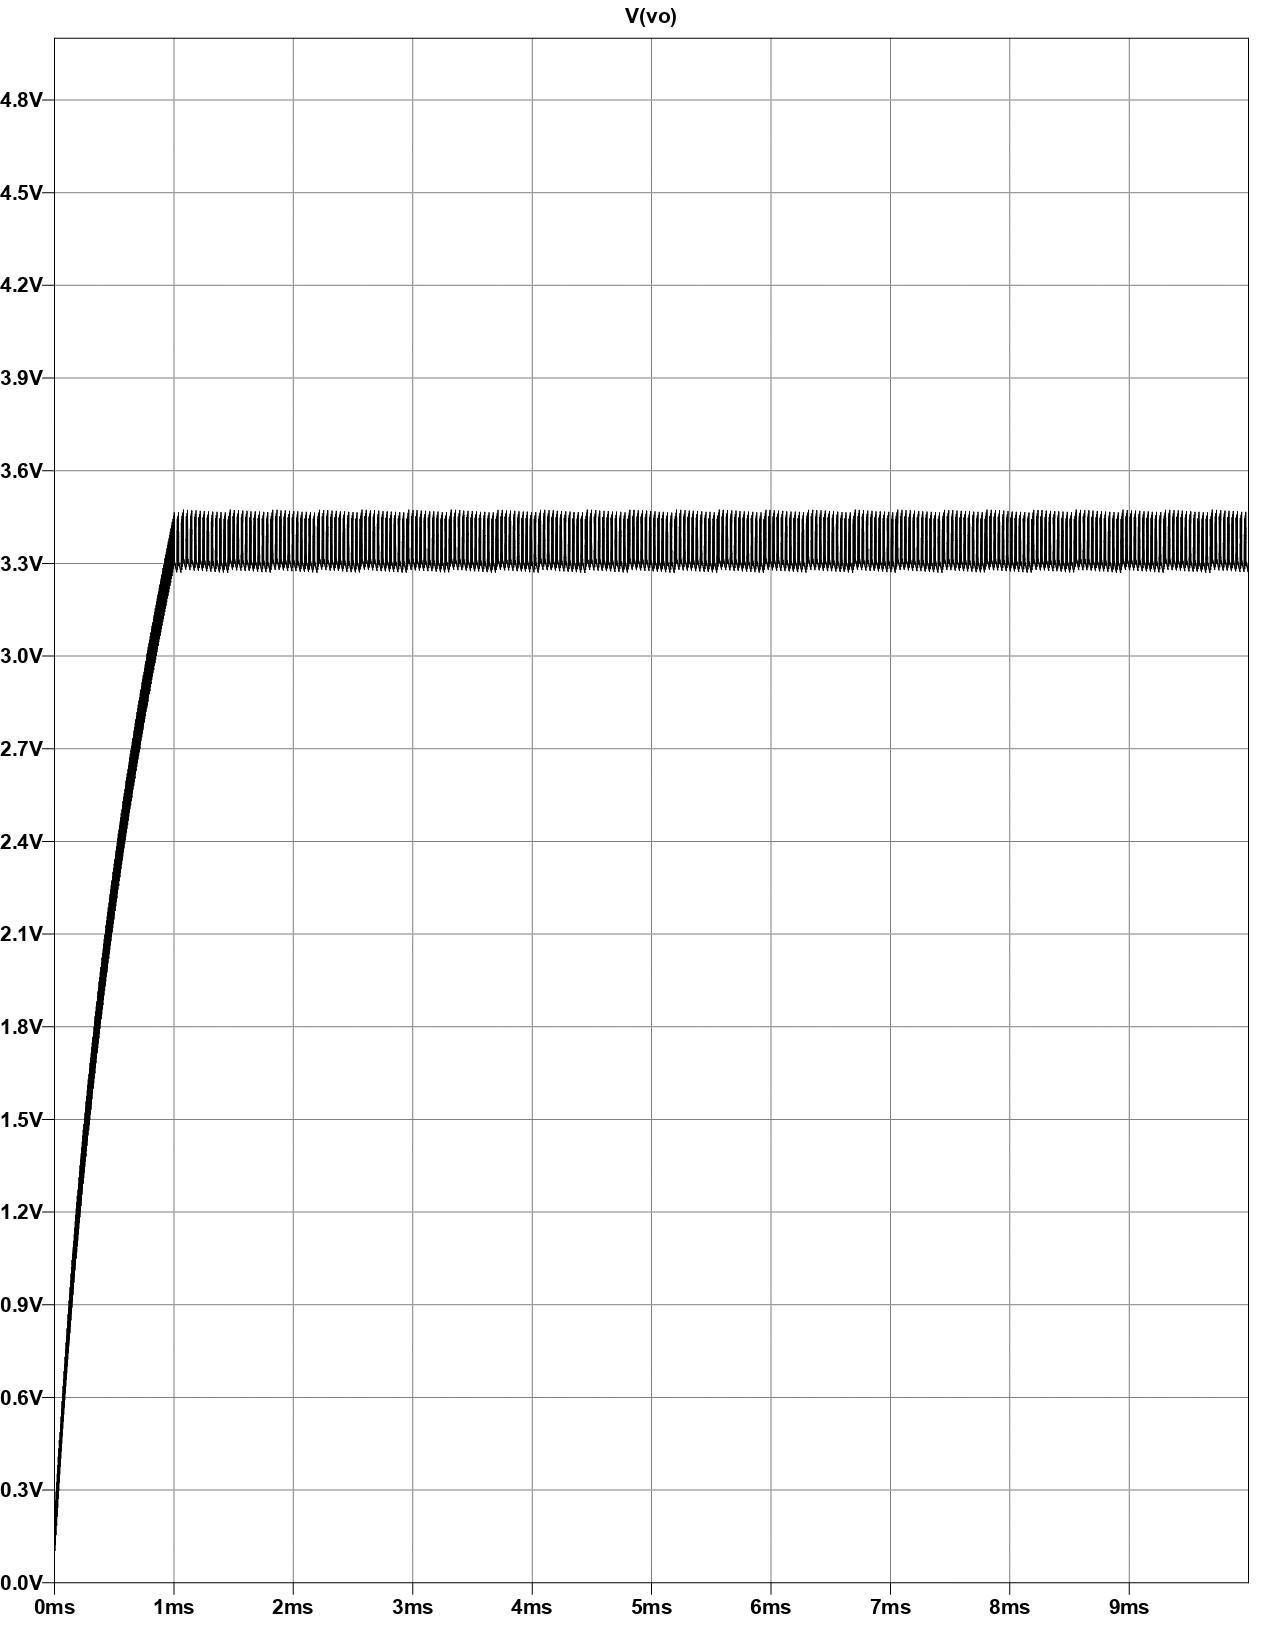
\includegraphics[width=\textwidth]{Pictures/Convertidor DC-DC MC34063A, 2s2p, bus 3.3 v a 750 mA_page-0001 Max.jpg}
    \caption{Salida de voltaje a 3.3 voltios. Vin máximo (8.4 V).}
    \label{fig:2s2p_33v_2dcdcconverters_Max}
  \end{subfigure}
  \hfill
  \begin{subfigure}{0.48\linewidth}
    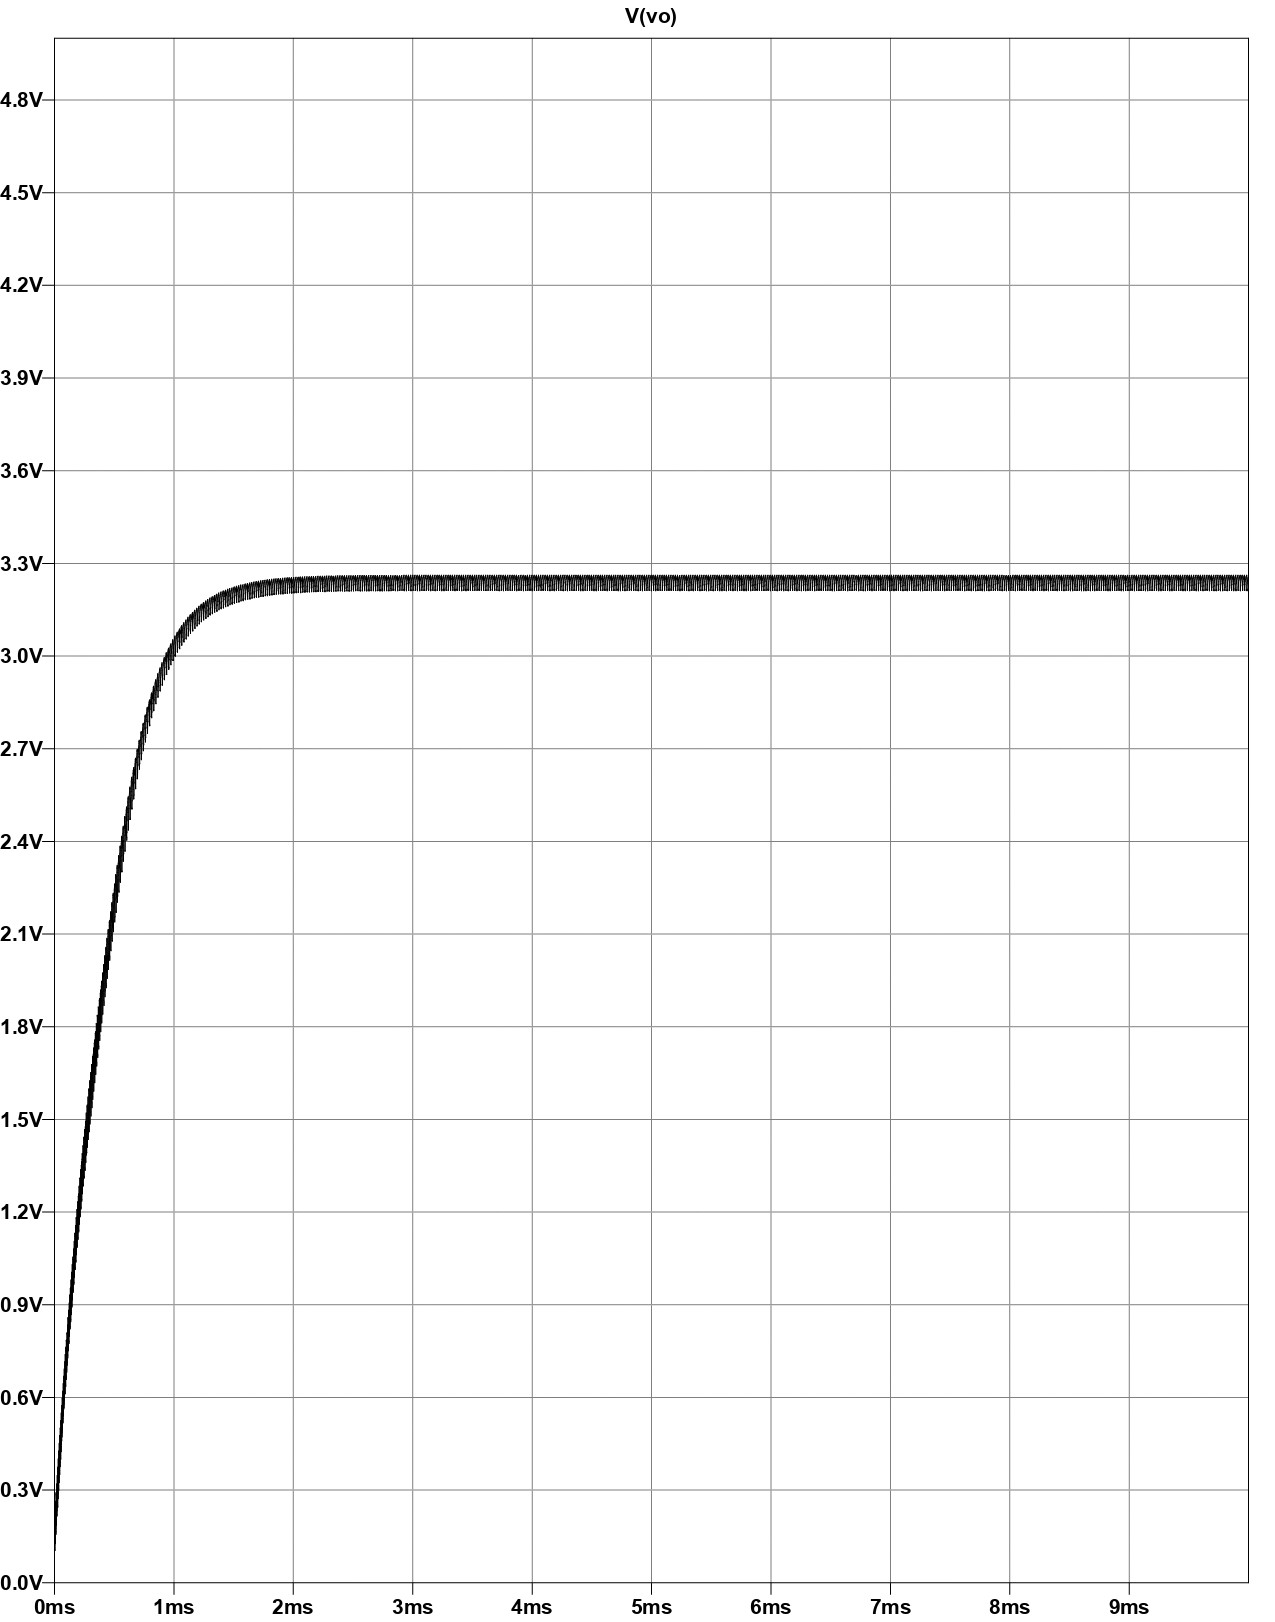
\includegraphics[width=\textwidth]{Pictures/Convertidor DC-DC MC34063A, 2s2p, bus 3.3 v a 750 mA_page-0001 Min.jpg}
    \caption{Salida de voltaje a 3.3 voltios. Vin mínimo operativo (5.5 V).}
    \label{fig:2s2p_33v_2dcdcconverters_min}
  \end{subfigure}
  \caption{Convertidor DC-DC MC34063A, arreglo 2s2p, bus de 3.3 V a 750 mA.}
\end{figure}

\newpage

Podemos observar que en ambos casos, los resultados son satisfactorios para alimentar las cargas. Tanto el valor pico a pico como el sobreimpulso se encuentran en niveles tolerables, lo que representa un resultado satisfactorio sin requerir el ajuste de la inductancia del filtro pasabajos.

Es importante mencionar que en el caso de la Figura \ref{fig:2s2p_33v_2dcdcconverters_min}, se considera como valor mínimo operativo 5.5V, ya que según simulaciones, este es el valor mínimo que el banco de baterías puede proporcionar para obtener una salida regulada de 3.3V. Sin embargo, según la hoja técnica del fabricante y la curva de descarga del modelo de batería Panasonic 18650b, esto se considera despreciable en términos de carga almacenada \cite{panasonic_18650b}.

% PARA EL BUS DE 5.0 VOLTIOS ************

Siguiendo un procedimiento similar, empleamos los cálculos de la Tabla \ref{tab:valores_50_2s2p}, y obtenemos los resultados de la Fig. \ref{fig:2s2p_50v_2dcdcconverters_Max} para un banco de baterías a máxima carga y la Fig. \ref{fig:2s2p_50v_2dcdcconverters_min} a mínima carga.

\begin{table*}[h]
    \centering
    \begin{tabular}{p{0.25\linewidth}p{0.1\linewidth}p{0.25\linewidth}p{0.1\linewidth}}
    \hline
    \textbf{Entradas} & \textbf{Valor} & \textbf{Salidas} & \textbf{Valor} \\ \hline
    Vin (min)[V] & 5.5 & Ct [pF] & 327 \\
    Vout [V] & 5.0 & Ipk [mA] & 1500 \\
    Iout [mA] & 500 & Rsc [Ohm] & 0.3 \\
    V ripple pp [mV] & 10 & Lmin [uH] & 10 \\
    Fmin [kHz] & 100 & Co [uF] & 125 \\
    ~ & ~ & R1 [kohm] & 1 \\
    ~ & ~ & R2 [kohm] & 3 \\ \hline
    \end{tabular}
\caption{Valores para convertidor DC-DC MC34063A, arreglo 2s2p, bus 5.0 V a 750 mA.}
\label{tab:valores_50_2s2p}
\end{table*}

Al analizar los resultados presentados en la Figura \ref{fig:arreglo2s2p5vdc}, se aprecia que en condiciones de máxima carga (Fig. \ref{fig:2s2p_50v_2dcdcconverters_Max}), no se logra alcanzar el voltaje deseado para la regulación, y esta situación se agrava en condiciones de mínima carga en el banco de baterías (Fig. \ref{fig:2s2p_50v_2dcdcconverters_min}). Esta discrepancia puede atribuirse a la diferencia entre el voltaje de entrada y el voltaje objetivo en este arreglo para el convertidor DC-DC .

Aunque en esta ocasión no se observan problemas relacionados con sobreimpulsos, este diseño no se considera adecuado para aplicaciones del EPS debido a que los valores de tensión necesarios no se alcanzan y, en consecuencia, los componentes electrónicos no funcionarían de manera óptima.


\begin{figure}[h]
  \centering
  \begin{subfigure}{0.48\linewidth}
    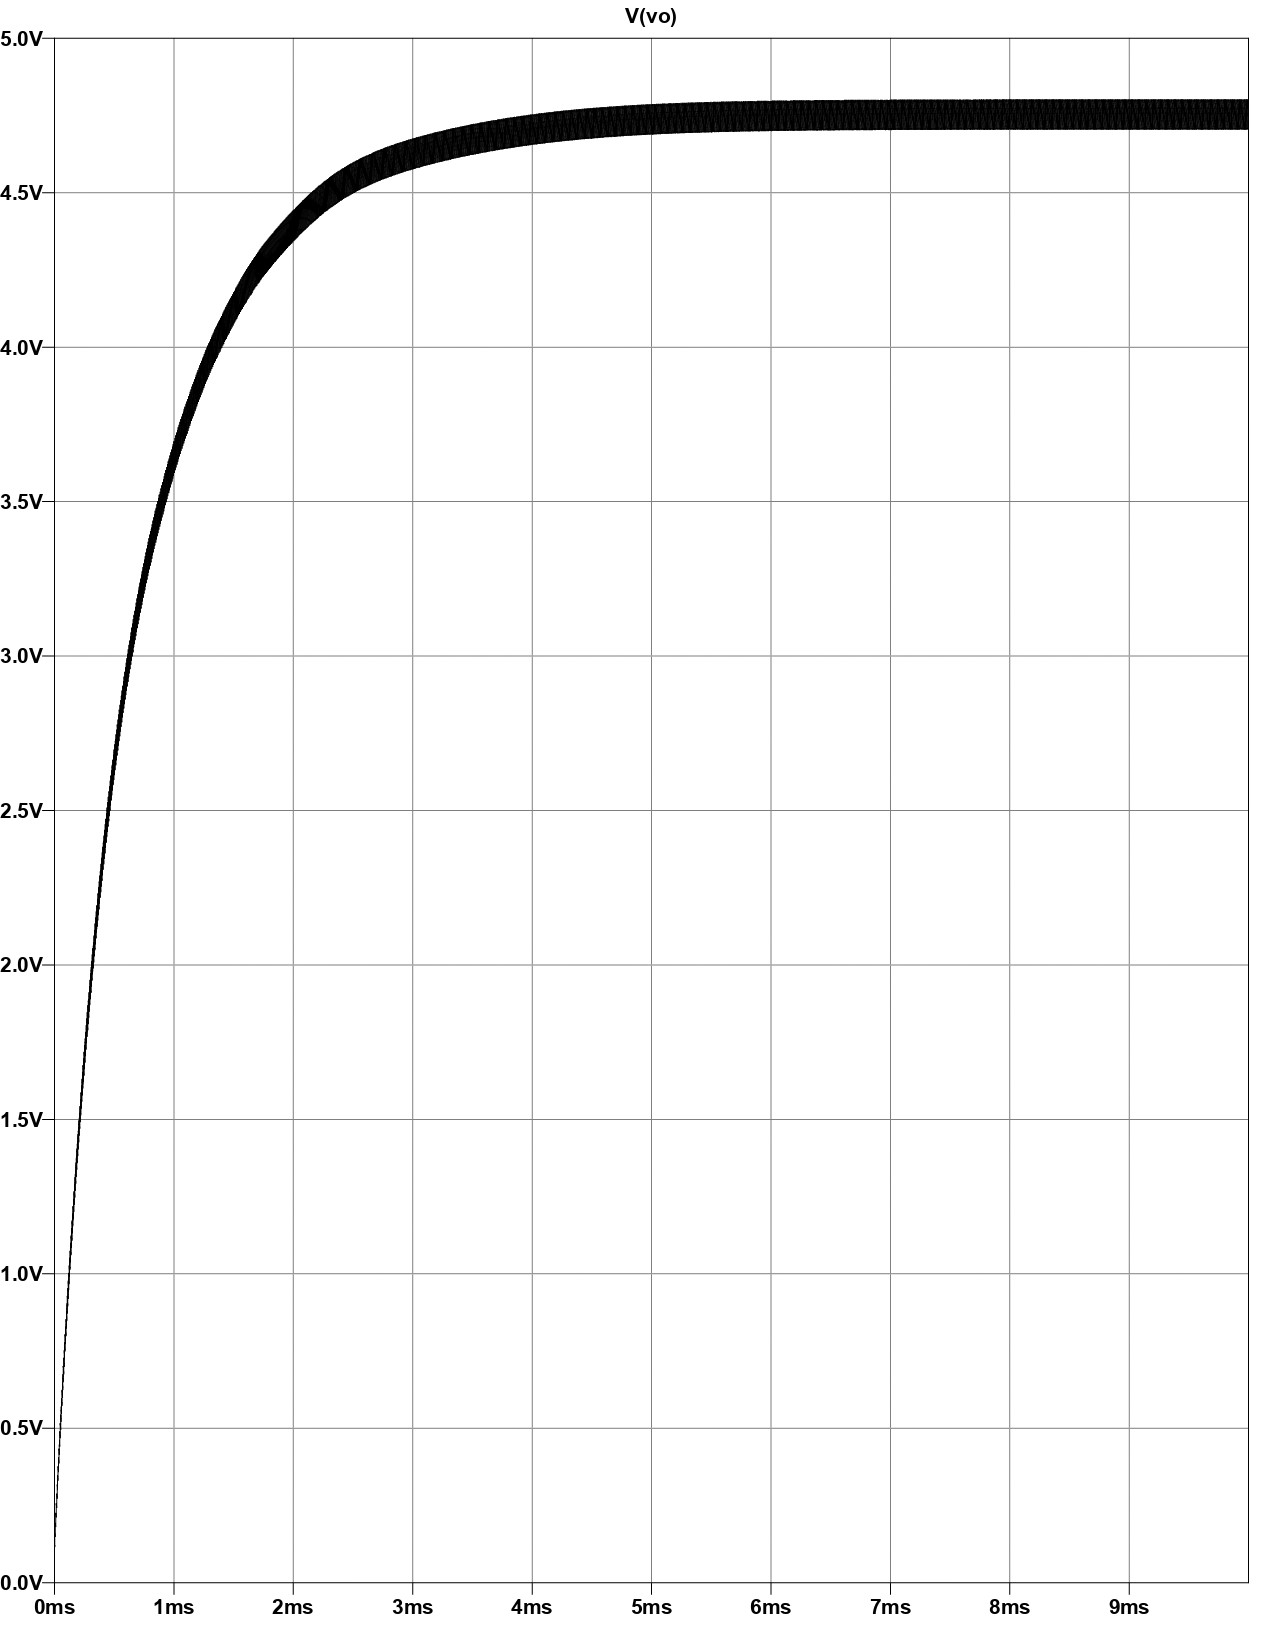
\includegraphics[width=\textwidth]{Pictures/Convertidor DC-DC MC34063A, 2s2p, bus 5.0 v a 500 mA_page-0001 Max.jpg}
    \caption{Salida de voltaje a 5.0 voltios. Vin máximo (8.4 V).}
    \label{fig:2s2p_50v_2dcdcconverters_Max}
  \end{subfigure}
  \hfill
  \begin{subfigure}{0.48\linewidth}
    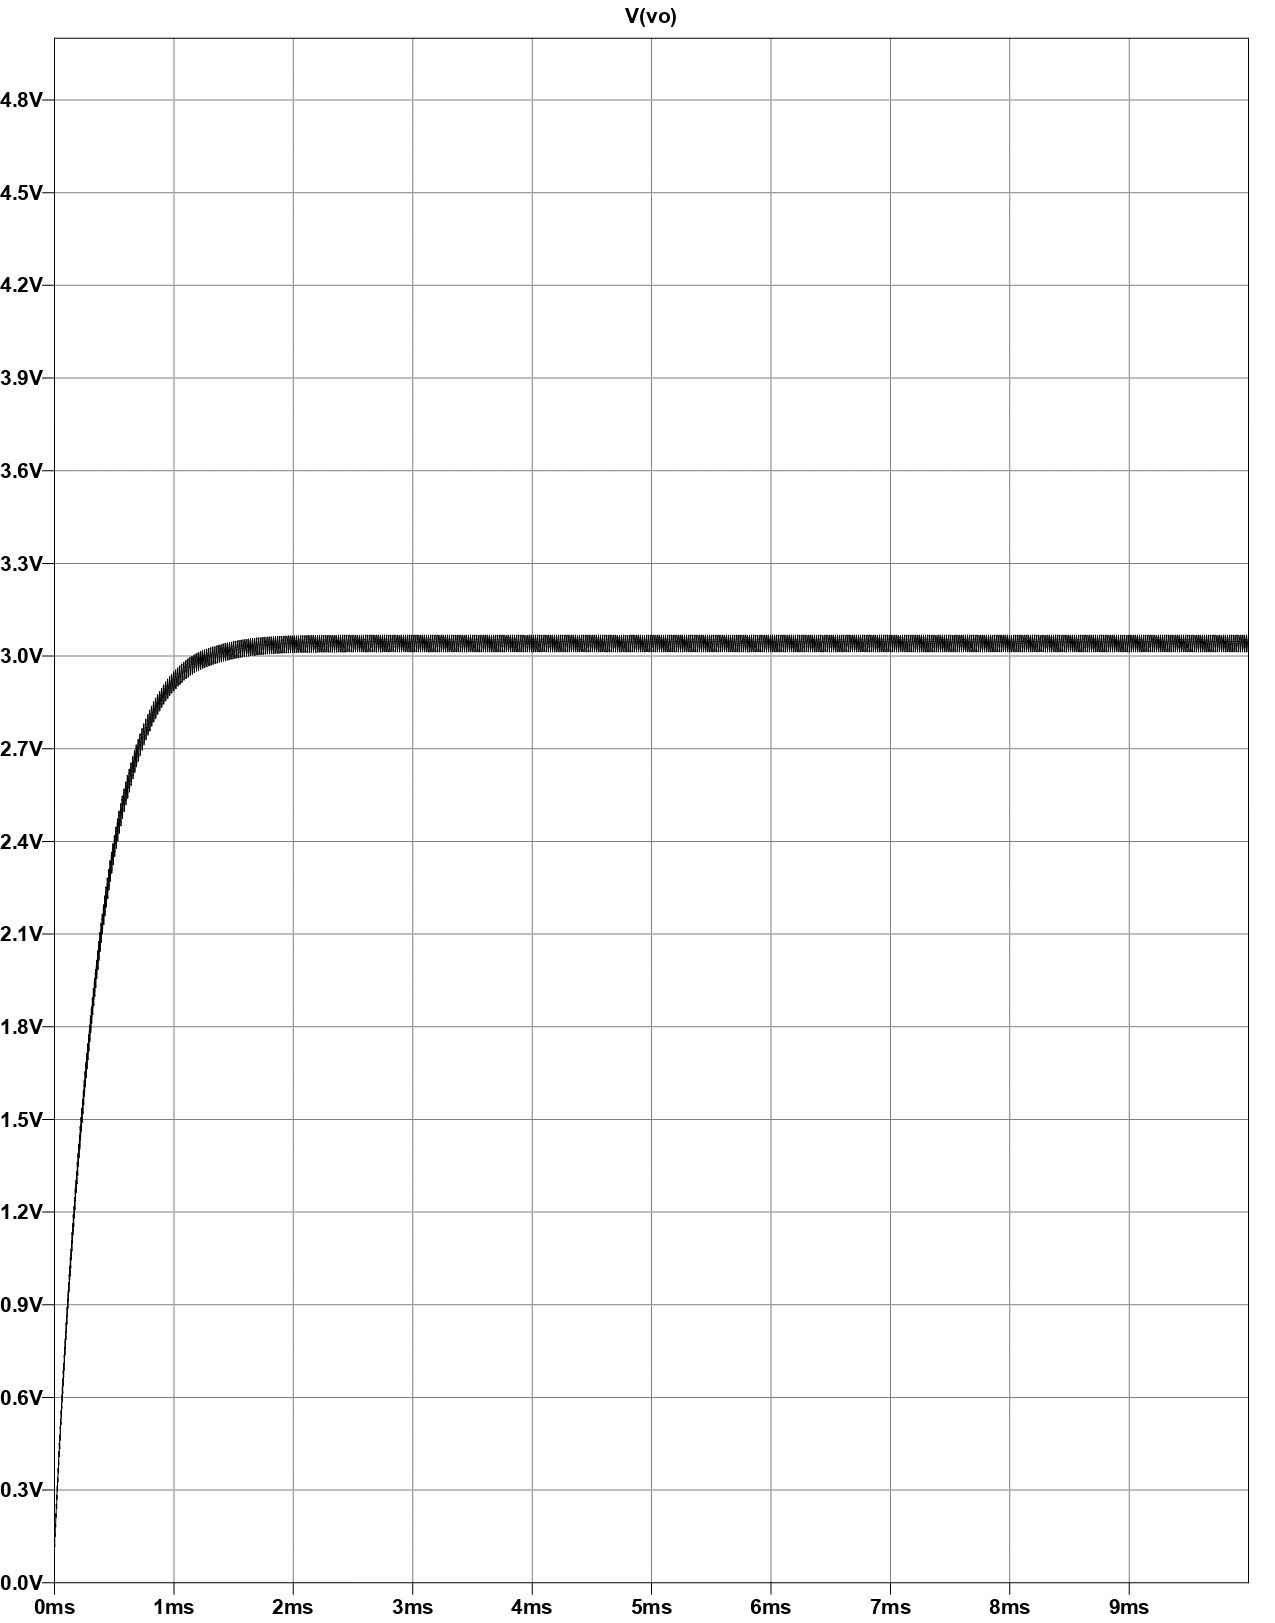
\includegraphics[width=\textwidth]{Pictures/Convertidor DC-DC MC34063A, 2s2p, bus 5.0 v a 500 mA_page-0001 Min.jpg}
    \caption{Salida de voltaje a 5.0 voltios. Vin mínimo operativo (5.5 V).}
    \label{fig:2s2p_50v_2dcdcconverters_min}
  \end{subfigure}
  \caption{Convertidor DC-DC MC34063A, arreglo 2s2p, bus de 5.0 V a 500 mA.}
  \label{fig:arreglo2s2p5vdc}
\end{figure}







% ARREGLO 1S4P
\subsection{Arreglo de baterías 1s4p}

Para esta configuración, es crucial considerar detenidamente la curva de descarga característica de una batería de litio. El fabricante, en el caso del modelo Panasonic NCR-18650B, proporciona una curva tentativa \cite{panasonic_18650b}. Sin embargo, para obtener mediciones más realistas, se requiere realizar pruebas de laboratorio. En este caso, nos apoyamos en las curvas de descarga a una temperatura ambiente de 20°C, obtenidas y evidenciadas en trabajos como el de Kopczynski en 2018 \cite{Kopczynski2018}. Estas mediciones se presentan en la Fig. \ref{fig:discharging_characteristic}.

\begin{figure}[h]
  \centering
  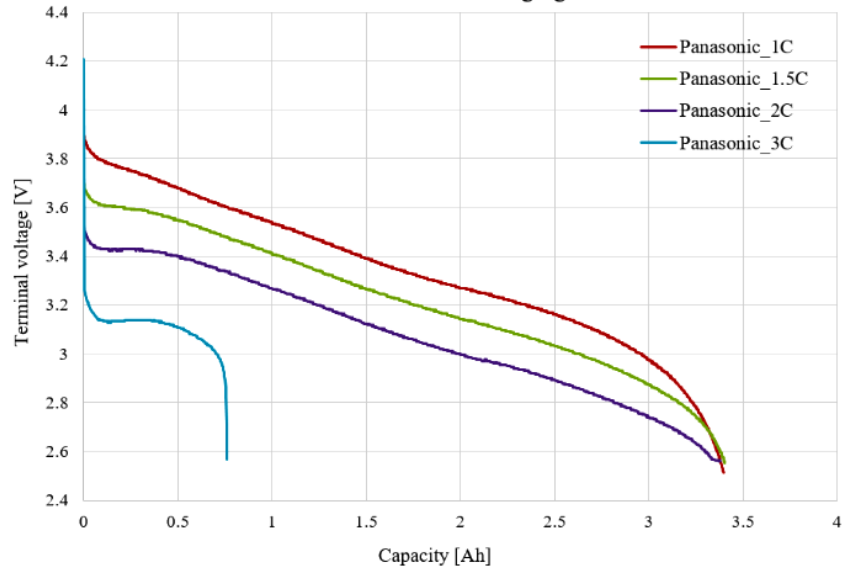
\includegraphics[width=0.45\linewidth]{Pictures/PanasonicCurveDischarge.png} 
  \caption{Discharging characteristic of Panasonic NCR-18650B battery with different discharging current at room temperature (20°C). Fuente: Adaptado de \cite{Kopczynski2018}, con licencia CC BY 4.0}
\label{fig:discharging_characteristic}
\end{figure}

\newpage

Como se evidencia en la Fig. \ref{fig:discharging_characteristic}, una configuración exclusivamente de reducción (buck) o exclusivamente de elevación (boost) resultaría insuficiente. Es en este punto donde surge la necesidad de implementar un convertidor DC-DC que pueda operar dinámicamente en ambos modos. Sin embargo, este enfoque implicaría un nivel de complejidad que excede el alcance de este trabajo de investigación. 

La implementación de tal sistema requeriría la utilización de un circuito integrado distinto al MC34063A, así como un diseño sustancialmente diferente. Por lo tanto, dadas las actuales exigencias del sistema de energía para una misión de globo de gran altitud (HAB), se ha decidido no explorar esta configuración del banco de baterías en el presente estudio.

\vspace{0.75 cm}

\subsection{Implementación de MC34063A en PCB}
\vspace{0.25 cm}
Luego de una minuciosa evaluación del convertidor DC-DC MC34063A en las configuraciones 4s1p, 2s2p y 1s4p, basada en los resultados detallados de las simulaciones en LTSPICE, se llega a la conclusión de que la configuración 4s1p presenta la respuesta más destacada. Tras ajustes precisos en la inductancia del filtro pasabajos, esta disposición exhibió un rendimiento excepcional en la salida, alcanzando el valor de voltaje requerido con un margen de error y un sobreimpulso prácticamente despreciables. Por consiguiente, se ha optado por seleccionar esta configuración para la implementación.

La ejecución de la implementación se llevará a cabo mediante el uso del software Fusion360 de Autodesk. Este programa se utilizará para el desarrollo del esquemático, el diseño de la PCB y el modelado 3D del convertidor DC-DC destinado al bus de 3.3V y 5.0V.\\\\ En las Figuras \ref{fig:MC34063A_Esquemático_33V}, \ref{fig:MC34063A_PCB_33V}, y \ref{fig:MMC34063A_3D_33V}, se presentan detalladamente los resultados obtenidos para el bus de 3.3V.


\newpage

\begin{figure}[h]
  \centering
  \includegraphics[width=0.9\linewidth]{Pictures/MC34063A_Esquemático_33V.png} 
  \caption{Esquemático del convertidor DC-DC con MC34063A. Entrada nominal de 14.4V, salida de 3.3V a 750 mA.}
  \label{fig:MC34063A_Esquemático_33V}
\end{figure}

\begin{figure}[h]
  \centering
  \includegraphics[width=0.52\linewidth]{Pictures/MC34063A_PCB_33V.png} 
  \caption{Diseño de PCB para el convertidor DC-DC con MC34063A. Entrada nominal de 14.4V, salida de 3.3V a 750 mA.}
  \label{fig:MC34063A_PCB_33V}
\end{figure}

\newpage

\begin{figure}[h]
  \centering
  \includegraphics[width=0.65\linewidth]{Pictures/MC34063A_3D_33V.jpeg} 
  \caption{Vista 3D de la PCB para el convertidor DC-DC con MC34063A. Entrada nominal de 14.4V, salida de 3.3V a 750 mA.}
  \label{fig:MMC34063A_3D_33V}
\end{figure}

Para el bus de 5.0V, se desarrollaron el esquemático, la PCB y modelado 3D del convertidor DC-DC, y se presentan en las Figuras \ref{fig:MC34063A_Esquemático_50V}, \ref{fig:MC34063A_PCB_50V} y \ref{fig:MC34063A_3D_50V}, respectivamente.






\begin{figure}[h]
  \centering
  \includegraphics[width=0.9\linewidth]{Pictures/MC34063A_Esquemático_50V.png} 
  \caption{Esquemático del convertidor DC-DC con MC34063A. Entrada nominal de 14.4V, salida de 5.0V a 750 mA.}
  \label{fig:MC34063A_Esquemático_50V}
\end{figure}

\newpage

\begin{figure}[h]
  \centering
  \includegraphics[width=0.55\linewidth]{Pictures/MC34063A_PCB_50V.png} 
  \caption{Diseño de PCB del convertidor DC-DC con MC34063A. Entrada nominal de 14.4V, salida de 5.0V a 750 mA.}
  \label{fig:MC34063A_PCB_50V}
\end{figure}

\begin{figure}[h]
  \centering
  \includegraphics[width=0.75\linewidth]{Pictures/MC34063A_3D_50V.png} 
  \caption{Vista 3D del diseño del convertidor DC-DC con MC34063A. Entrada nominal de 14.4V, salida de 5.0V a 750 mA.}
  \label{fig:MC34063A_3D_50V}
\end{figure}

\newpage

\section{Revisión de autoconsumo de EPS}

Tras dimensionar los componentes del EPS, es crucial evaluar el autoconsumo por dos razones: validar el dimensionamiento inicial del banco de baterías y determinar la corriente efectiva de los convertidores DC-DC. Los detalles del consumo energético se encuentran en las Tablas \ref{tab:autoconsumo50_EPS} y \ref{tab:autoconsumo33_EPS}.




\begin{table}[!ht]
    \centering
    \renewcommand{\arraystretch}{1.2}
    \caption{Cuadro de cargas para autoconsumo de EPS, bus 5.0 V}
    \label{tab:autoconsumo50_EPS}
    \begin{tabularx}{1.1\textwidth}{lllllll}
    \hline
    \textbf{Descripción} & \textbf{Cantidad} & \textbf{I [mA]} & \textbf{P [W]} & \textbf{t [h]} & \textbf{E [Wh]} & \textbf{Q [mAh]} \\
    \hline
    MCU & 1 unidad & 180.00 & 0.900 & 6.00 & 5.40 & 1080.00 \\ 
    MOSFET & 1 unidad & 33.00 & 0.165 & 6.00 & 0.99 & 198.00  \\ 
    MS5611 & 1 unidad & 1.4 & 0.00 & 6.00 & 0.04 & 8.40  \\ 
    ACS723 & 1 unidad & 1.00 & 0.00& 6.00 & 0.03& 6.00  \\ 
    ADC & 2 unidad & 80.00 & 0.40 & 6.00 & 0.24 & 480.00 \\
    \hline
    & & \textbf{I Máx.} & 295.40 & &\textbf{Q Total.} & 1772.40 \\ 
    \hline
    \end{tabularx}
\end{table}


\begin{table}[!ht]
    \centering
    \renewcommand{\arraystretch}{1.2}
    \caption{Cuadro de cargas para autoconsumo de EPS, bus 3.3 V}
    \label{tab:autoconsumo33_EPS}
    \begin{tabularx}{1.1\textwidth}{lllllll}
    \hline
    \textbf{Descripción} & \textbf{Cantidad} & \textbf{I [mA]} & \textbf{P [W]} & \textbf{t [h]} & \textbf{E [Wh]} & \textbf{Q [mAh]} \\
    \hline
    MOSFET & 1 unidad & 33.00 & 0.01 & 6.00 & 0.6 & 120.00 \\
    \hline
    & & \textbf{I Máx.} & 33.00 & &\textbf{Q Total.} & 120.00 \\ 
    \hline
    \end{tabularx}
\end{table}

En el capítulo III, sección en la que se desarrolló un presupuesto energético, estimamos inicialmente una corriente de 983 mA y un consumo en carga de 5519 mAh para el bus de 3.3 V. Para el bus de 5.0 V, se estimó una corriente de 402 mA y un consumo en carga de 1326 mAh.

Considerando el autoconsumo del EPS (ver la Tabla \ref{tab:autoconsumo50_EPS} y Tabla \ref{tab:autoconsumo33_EPS}), actualizamos estos valores de la siguiente manera: el bus de 3.3 V tendría una corriente de 1016 mA con una necesidad en carga de 5639 mAh. En cuanto al bus de 5.0 V, la corriente sería de 698 mA y la carga de 3098 mAh.

Estas cifras son mejores para dimensionar las protecciones eléctricas. La necesidad total de carga es de 8737 mAh, pero aún no hemos considerado la eficiencia de los convertidores DC-DC (aproximadamente 83.7\% según el fabricante \cite{ti_mc34063a}). Esto nos lleva a una carga necesaria de 10439 mAh. Comparando con la capacidad nominal del arreglo 4s1p de 13600 mAh, concluimos que el banco de baterías sigue siendo capaz, al 77\% de su capacidad.



\section{Dispositivos de Protección Eléctrica}

Las baterías de iones de litio, debido a su alta densidad energética, requieren un manejo cauteloso. En el mercado actual, los circuitos integrados (IC) especializados abordan consideraciones críticas de seguridad, destacando:

\begin{itemize}
    \item \textbf{Sobrecarga:} Las baterías deben cargarse hasta 4.1 V o 4.2 V/celda de manera segura. Un circuito de protección evita daños y riesgos de incendio.
    \item \textbf{Sobre-descarga:} Evita descargar las baterías por debajo de 2.5 V/celda para preservar su vida útil.
    \item \textbf{Descarga rápida:} Los IC desconectan la batería ante corrientes de descarga excesivas.
\end{itemize}

Los IC de protección utilizan MOSFET para gestionar la conexión y desconexión de celdas de litio. Permiten la conexión en paralelo de celdas del mismo tipo, compartiendo eficientemente el circuito de protección \cite{knight2015lithium}.

Para este trabajo de investigación, consideraremos dos alternativas, una orientada al caso de implementar un cargador a bordo, y la otra considerando únicamente el proceso de descarga, es decir un limitador de corriente. Además, como medida de protección adicional, los interruptores mecánicos pueden ser una buena adición al diseño, reduciendo aún más el riesgo de encendidos accidentales del sistema previo a la misión. 

\subsection{Protección eléctrica para cargador a bordo}

Las consideraciones críticas de sobrecarga, sobre-descarga y descarga rápida son abordadas integralmente en este enfoque de protección eléctrica, especialmente diseñado para un flujo bidireccional de potencia, tanto desde el banco de baterías hacia las cargas como del cargador hacia las baterías.

Para la implementación práctica en proyectos de potencia a escala, con énfasis en la economía y accesibilidad, se destaca el uso del circuito integrado AP9101C de Diodes Incorporated.

El AP9101C, un IC de protección altamente preciso, está diseñado para salvaguardar baterías al detectar sobrecargas, sobredescargas y otros eventos anómalos. Su bajo consumo de corriente, precisión en la detección de voltajes y circuito de tiempo incorporado minimizan la necesidad de componentes externos. Se presenta como una opción eficiente y precisa para la protección de baterías. La Tabla \ref{tab:ap9101} detalla sus características. En cuanto al esquemático, el fabricante ofrece una configuración \cite{diodes2023ap9101c}.




\begin{table}[h]
    \centering
    \caption{Parámetros Clave AP9101C}
    \begin{tabular}{l|l}
        \hline
        \textbf{Baja Corriente de Consumo} & \begin{tabular}[c]{@{}l@{}}3.0µA Typ. (Modo de Operación, VDD = 3.5V)\\ 0.01µA Typ. (Modo de Apagado)\end{tabular} \\ \hline
        \textbf{Circuito de Detección de Voltaje} & \begin{tabular}[c]{@{}l@{}}Alta Precisión a +25°C\\ Sobrecarga: 3.5V a 4.5V (±25mV)\\ Sobre descarga: 2.0V a 3.4V (±35mV)\end{tabular} \\ \hline
        \textbf{Rango de Voltaje de Histéresis} & \begin{tabular}[c]{@{}l@{}}Sobrecarga: 0.1V a 0.4V (±50mV)\\ Sobre descarga: 0V a 0.7V (±65mV)\end{tabular} \\ \hline
        \textbf{Sobrecorriente de Descarga} & \begin{tabular}[c]{@{}l@{}}Voltaje de Detección: 0.05V a 0.32V (±15mV)\\ Corriente Corta: 0.45V a 0.7V (±100mV)\end{tabular} \\ \hline
        \textbf{Sobrecorriente de Carga} & \begin{tabular}[c]{@{}l@{}}Voltaje de Detección: -0.2V a -0.05V (±15mV)\\ Detección de Sobrecargador: 8.0V (Fijo, ±2V)\\ Liberación de Sobrecargador: 7.3V (Fijo, ±2V)\end{tabular} \\ \hline
    \end{tabular}
    \label{tab:ap9101}
\end{table}

\begin{figure}[h]
  \centering
  \includegraphics[width=\linewidth]{Pictures/AP9101C.png} 
  \caption{Esquemático de circuito de protección AP9101C \cite{diodes2023ap9101c}. Los valores son los sugeridos por el fabricante. El modelo MOSFET se recomienda el modelo DMG6968 de Diodes Incorporated.}
  \label{fig:EsquematicoAP9101C}
\end{figure}

\newpage
\subsection{Protección eléctrica como limitador de corriente}

En el contexto de una misión de globo de gran altitud con un período operativo breve, donde no se realizarán ciclos de carga y descarga del banco de baterías, se buscan protecciones específicas. Dado que el escenario se limita principalmente a la descarga de las baterías, las medidas de protección se orientan hacia la preparación ante eventos como cortocircuitos. Una alternativa adecuada es la implementación de circuitos conocidos como limitadores de corriente, como el IC comercial LTC4361 de Analog Devices \cite{LTC4361}, el cual utilizaremos en este trabajo. Las especificaciones técnicas de este dispositivo se detallan en la Tabla \ref{tab:especificaciones_LTC4361}.




\begin{table}[h]
  \centering
  \caption{Especificaciones de LTC4361}
  \begin{tabular}{l|l}
    \hline
    \textbf{Característica} & \textbf{Valor} \\
    \hline
    Rango de Operación & 2.5V a 5.5V \\
    Protección contra Sobretensión & Hasta 80V \\
    No se Requiere Condensador de Entrada o TVS & Para la mayoría de las aplicaciones \\
    Umbral de Sobretensión Preciso & 5.8V con 2\% de precisión \\
    Interruptor de Circuito de Sobrecorriente & 50mV con 10\% de precisión \\
    Apagado por Sobretensión <1µs & Apagado suave \\
    \hline
  \end{tabular}
  \label{tab:especificaciones_LTC4361}
\end{table}

Para la implementación del LTC4361, la hoja técnica propone un esquemático y establece que el dispositivo regula su valor de disparo para la protección mediante un ajuste de corriente, que se determina a partir de la ecuación \ref{eq:LTC4361}.

\begin{equation}\label{eq:LTC4361}
    R_{\text{sense}} = \frac{\Delta V_{\text{oc}}}{I_{\text{trip}}}
\end{equation}


Donde:
\begin{itemize}
    \item $\Delta V_{\text{oc}}$ tiene un valor de 50mV.
    \item $I_{\text{trip}}$ es la corriente de disparo.
\end{itemize}

Sabemos que la corriente de operación estimada para el bus de 3.3 V es de 1016 mA, mientras que para el bus de 5.0 V es de 698 mA. Sin embargo, la consideración de esta información no es el único aspecto crucial. También debemos tener en cuenta que el diseño de las protecciones se orienta a prevenir daños en los sistemas electrónicos. En particular, se enfoca en proteger el material conductor, que en este caso corresponde a las pistas de los circuitos. Para este trabajo, se ha tomado un espesor general de 0.762 mm o 30 milésimas de pulgada (mil) para cada diseño de PCB.

Este valor se seleccionó considerando el material utilizado, que es FR-4. Según la tabla proporcionada por la compañía Altium para PCB con material FR-4, que sigue la norma definida por la NEMA (National Electrical Manufacturers Association) para un compuesto de resina epoxídica reforzada con fibra de vidrio, el espesor de 0.762 mm corresponde a una capacidad de corriente de 2 A. Esta información detallada se puede consultar en la Tabla \ref{tab:relacion_corriente_grosor}, que ofrece una referencia específica para el diseño de las pistas.

\begin{table}[h]
    \centering
    \caption{Relación entre la corriente y el grosor de la pista.}
    \label{tab:relacion_corriente_grosor}
    \begin{tabular}{ll}
        \hline
        Corriente (A) & Grosor de pista (mil) \\ 
        \hline
        1 & 10 \\ 
        2 & 30 \\ 
        3 & 50 \\ 
        4 & 80 \\ 
        5 & 110 \\ 
        6 & 150 \\ 
        7 & 180 \\ 
        8 & 220 \\ 
        9 & 260 \\ 
        10 & 300 \\ 
        \hline
    \end{tabular}
\end{table}

Dicho esto, se tomará un punto intermedio entre la capacidad de las pistas en las PCB (2 amperios) y la corriente estimada en el bus de mayor demanda (1 amperio). Por lo tanto, la corriente configurada como sobrecorriente o corriente de disparo de protecciones será de 1.5 amperios. Dando como resultado de la \ref{eq:LTC4361} un valor de $R_{sense}$ de 0.33 ohm.

Una vez definida la corriente de disparo, el esquemático está completo de acuerdo con la hoja técnica del fabricante \cite{LTC4361}, ver Fig. \ref{fig:Esquematico_LTC4361}, el diseño 2D de la PCB en la Fig. \ref{fig:PCB_LTC4361}y la vista 3D en la Fig.\ref{fig:3D_LTC4361}. 

\newpage

\begin{figure}[h]
  \centering
  \includegraphics[width=\linewidth]{Pictures/Esquematico_LTC4361.png} 
  \caption{Esquemático de circuito de protección LT4361 \cite{LTC4361}. Los valores son los sugeridos por el fabricante. Se calculó \(R_{\text{sense}} = 0.33 \ \Omega\) para \(I_{\text{trip}} = 1.5 \ \text{A}\).}
  \label{fig:Esquematico_LTC4361}
\end{figure}
\vspace{1 cm}
\begin{figure}[h]
  \centering
  \begin{subfigure}[b]{0.55\textwidth}
    \includegraphics[width=\linewidth]{Pictures/PCB_LTC4361.png}
    \caption{PCB de circuito de protección LTC4361}
    \label{fig:PCB_LTC4361}
  \end{subfigure}%
  \begin{subfigure}[b]{0.55\textwidth}
    \includegraphics[width=\linewidth]{Pictures/3D_LTC4361.png}
    \caption{Vista 3D de PCB de protección LTC4361}
    \label{fig:3D_LTC4361}
  \end{subfigure}
  \caption{PCB y Vista 3D del circuito de protección LTC4361}
  \label{fig:combinada_LTC4361}
\end{figure}

\newpage
\subsection{Sistemas de Desconexión y Seguridad}

En esta categoría, se exploran dos mecanismos esenciales. El primero consiste en un interruptor de 4 polos con 2 posiciones para cada uno (Fig. \ref{fig:4polosinterruptor}). Este diseño permite la desconexión individual de cada pila 18650, brindando la capacidad de aislar completamente el banco de baterías del resto del circuito y entre el arreglo de las pilas mismas.

\begin{figure}[h]
  \centering
  \includegraphics[width=0.3\linewidth]{Pictures/Interruptor.jpg} 
  \caption{Interruptor de 4 polos uxcell}
  \label{fig:4polosinterruptor}
\end{figure}

Como segundo sistema de seguridad, se implementa un enfoque similar al utilizado en misiones espaciales: un interruptor 'Remove Before Flight' (Fig. \ref{fig:figuraPrincipal}). Este interruptor actúa como un punto de control adicional contra posibles fallos y para prevenir activaciones no deseadas del sistema. Su adopción se basa en las mejores prácticas de seguridad y la experiencia acumulada en entornos críticos, donde prevenir errores humanos es de suma importancia.

\begin{figure}[h]
  \centering
  \begin{subfigure}{0.3\linewidth}
    \includegraphics[width=\linewidth]{Pictures/rbfinterruptor.jpg}
    \caption{Configuración}
    \label{fig:subfiguraA}
  \end{subfigure}
  \hspace{1cm} % Espacio horizontal entre las subfiguras
  \begin{subfigure}{0.3\linewidth}
    \includegraphics[width=\linewidth]{Pictures/rbfitems.png}
    \caption{Elementos}
    \label{fig:subfiguraB}
  \end{subfigure}
  \caption{Interruptor "Remove before flight \cite{labralab_pull_pin_switch_kit_2023}}
  \label{fig:figuraPrincipal}
\end{figure}

Ambos mecanismos de protección se conectan en serie, lo que implica que deben activarse secuencialmente para permitir el funcionamiento del sistema. Esta configuración en serie garantiza un doble nivel de seguridad, ya que ambas barreras deben superarse manualmente antes de que el sistema pueda operar.









\chapter{Integración de Sistemas}
En este capítulo, se aborda la fase de integración del sistema. Previamente, en el diseño e implementación, se llevaron a cabo diseños, simulaciones y PCB asociadas a las etapas que componen el sistema de energía desarrollado en este trabajo de investigación. En este punto, se busca integrar cada una de las etapas, siguiendo la lógica funcional establecida en la arquitectura del sistema. Se alcanza un nivel de conexiones físicas mediante el desarrollo de esquemáticos y, finalmente, el diseño de dos PCB de 12x8 cm, de acuerdo con los requisitos estructurales inicialmente definidos en los requerimientos.

\hspace{1.27cm}Adicionalmente, se aborda la integración a nivel de software mediante un flujograma que describe la lógica de programación requerida para la operación del sistema (ver Fig. \ref{fig:flujograma_EPS})

\hspace{1.27cm}Como resultado, obtenemos esquemáticos, los cuales se han dividido en cinco partes (Fig.\ref{fig:EPS_Sheet1} a Fig. \ref{fig:EPS_Sheet5}) y PCB del Sistema (ver Fig. \ref{fig:EPS_Final1} a Fig. \ref{fig:EPS_Final4}), integrando cada una de sus etapas, a nivel de hardware y software.


\newpage


\section{Software}

\begin{figure}[h]
  \centering
  \includegraphics[width=\textwidth]{Pictures/Flujograma_EPS.png}
  \caption{Flujograma de algoritmo de programación para EPS}
  \label{fig:flujograma_EPS}
\end{figure}

\newpage





\section{Hardware}

\begin{figure}[h]
  \centering
  \includegraphics[width=0.955\textwidth]{Pictures/EPS_Sheets_page-0001.jpg}
  \caption{Esquemático de EPS Integrado, Parte I.}
  \label{fig:EPS_Sheet1}
\end{figure}
\newpage

\begin{figure}[h]
  \centering
  \includegraphics[width=\textwidth]{Pictures/EPS_Sheets_page-0002.jpg}
  \caption{Esquemático de EPS Integrado, Parte II.}
  \label{fig:EPS_Sheet2}
\end{figure}
\newpage
\begin{figure}[h]
  \centering
  \includegraphics[width=\textwidth]{Pictures/EPS_Sheets_page-0003.jpg}
  \caption{Esquemático de EPS Integrado, Parte III.}
  \label{fig:EPS_Sheet3}
\end{figure}

\newpage
\begin{figure}[h]
  \centering
  \includegraphics[width=\textwidth]{Pictures/EPS_Sheets_page-0004.jpg}
  \caption{Esquemático de EPS Integrado, Parte IV.}
  \label{fig:EPS_Sheet4}
\end{figure}

\newpage
\begin{figure}[h]
  \centering
  \includegraphics[width=\textwidth]{Pictures/EPS_Sheets_page-0005.jpg}
  \caption{Esquemático de EPS Integrado, Parte V.}
  \label{fig:EPS_Sheet5}
\end{figure}

\newpage
\begin{figure}[h]
  \centering
  \includegraphics[width=\textwidth]{Pictures/EPS_FINAL.png}
  \caption{Vista frontal 3D de PCB 1 del EPS.}
  \label{fig:EPS_Final1}
\end{figure}

\begin{figure}[h]
  \centering
  \includegraphics[width=\textwidth]{Pictures/EPS_FINAL2.png}
  \caption{Vista trasera 3D de PCB 1 del EPS.}
  \label{fig:EPS_Final2}
\end{figure}
\newpage

\begin{figure}[h]
  \centering
  \includegraphics[width=\textwidth]{Pictures/EPS_FINAL4.png}
  \caption{Vista frontal 3D de PCB 2 del EPS.}
  \label{fig:EPS_Final3}
\end{figure}

\begin{figure}[h]
  \centering
  \includegraphics[width=\textwidth]{Pictures/EPS_FINAL3.png}
  \caption{Vista trasera 3D de PCB 2 del EPS.}
  \label{fig:EPS_Final4}
\end{figure}
\newpage



\chapter{Validación y Verificación del Sistema}

En este capítulo, se aborda la validación del Sistema de Energía (EPS), donde se llevan a cabo pruebas detalladas para verificar el cumplimiento de los requisitos establecidos previamente. Estas pruebas abarcan diversas áreas, incluyendo condiciones ambientales (Tabla \ref{tab:enviromentaltest}), parámetros eléctricos (Tabla \ref{tab:voltagecurrentmeasurement}), masa y longitud (Tablas \ref{tab:MassMeasurement} y \ref{tab:dimensionmeasurement}), comunicación entre subsistemas (Tabla \ref{tab:communicationtests}), control ON/OFF de carga útil (Tabla \ref{tab:payloadcontroltest}), y el correcto funcionamiento del sistema de carga y protecciones (Tabla \ref{tab:electricprotectioncharger}).

Cada una de estas pruebas sirve como un mecanismo de verificación acorde a los requerimientos establecidos previamente en la Tabla \ref{tab:requerimientos-eps}. Para este trabajo, se emplean principalmente simulaciones ambientales y SPICE para evaluar el comportamiento de los componentes electrónicos.


\newpage

\begin{table}[h]
    \centering
    \begin{tabular}{|m{6.5cm}|m{6.5cm}|}
    \hline
        \textbf{ID de Prueba} & \textbf{Descripción} \\ \hline
        \centering R1 & Ensayo de vacío térmico. Se somete la estructura a un test de vacío térmico (ver Anexo \ref{ap:CONESCAPAN_XL}) y se toman mediciones de temperatura y presión al interior de la estructura que protege al EPS. \\ \hline
        \multicolumn{2}{|m{13cm}|}{\centering\textbf{Mediciones a realizar}} \\ \hline
        \textbf{Variable medida} & \textbf{Valor medido} \\ \hline
        Temperatura Mínima alcanzada [\degree C]  (De -20 \degree C hasta 60 \degree C) & ~ \\ \hline
        Temperatura Máxima alcanzada [\degree C]  (De -20 \degree C hasta 60 \degree C) & ~ \\ \hline
        Tiempo de autonomía a una descarga de 1C  [h] (1 hora a 3.4 A) $\pm$ 5\% & ~ \\ \hline
    \end{tabular}
    \caption{Prueba ambiental}
    \label{tab:enviromentaltest}
\end{table}

\begin{table}[h]
    \centering
    \begin{tabular}{|m{6.5cm}|m{6.5cm}|}
    \hline
        \textbf{ID de Prueba} & \textbf{Descripción} \\ \hline
        \centering R2 y R3 & Medición de voltaje y corriente en Bus de 5.0 V y 3.3 V para corroborar una tensión estable a 750 mA de demanda. \\ \hline
        \multicolumn{2}{|m{13cm}|}{\centering\textbf{Mediciones a realizar}} \\ \hline
        \textbf{Variable medida} & \textbf{Valor medido} \\ \hline
        Voltaje [V] (3.3V $\pm$ 1\% a 750 mA) & ~ \\ \hline
        Voltaje [V] (3.3V $\pm$ 1\% a 250 mA) & ~ \\ \hline
        Voltaje [V] (3.3V $\pm$ 1\% a 500 mA) & ~ \\ \hline
        Voltaje [V] (5.0V $\pm$ 1\% a 750 mA) & ~ \\ \hline
        Voltaje [V] (5.0V $\pm$ 1\% a 500 mA) & ~ \\ \hline
        Voltaje [V] (5.0V $\pm$ 1\% a 250 mA) & ~ \\ \hline
    \end{tabular}
    \caption{Prueba de Parámetros Eléctricos}
    \label{tab:voltagecurrentmeasurement}
\end{table}

\newpage

\begin{table}[h]
    \centering
    \begin{tabular}{|m{6.5cm}|m{6.5cm}|}
    \hline
        \textbf{ID de Prueba} & \textbf{Descripción} \\ \hline
        \centering R4 & Medición de masa del EPS completo. \\ \hline
        \multicolumn{2}{|m{13cm}|}{\centering\textbf{Mediciones a realizar}} \\ \hline
        \textbf{Variable medida} & \textbf{Valor medido} \\ \hline
        Masa [g] (Menor a 600 gramos) & ~ \\ \hline
    \end{tabular}
    \caption{Prueba de Masa}
    \label{tab:MassMeasurement}
\end{table}



\begin{table}[h]
    \centering
    \begin{tabular}{|m{6.5cm}|m{6.5cm}|}
    \hline
        \textbf{ID de Prueba} & \textbf{Descripción} \\ \hline
        \centering R5 & Medición de longitud de EPS. \\ \hline
        \multicolumn{2}{|m{13cm}|}{\centering\textbf{Mediciones a realizar}} \\ \hline
        \textbf{Variable medida} & \textbf{Valor medido} \\ \hline
        Cantidad (Máx. 2 PCB) & ~ \\ \hline
        Dimensiones (12 cm x 8 cm x 2.5 cm) & ~ \\ \hline
    \end{tabular}
    \caption{Prueba de Longitud}
    \label{tab:dimensionmeasurement}
\end{table}



\begin{table}[h]
    \centering
    \begin{tabular}{|m{6.5cm}|m{6.5cm}|}
    \hline
        \textbf{ID de Prueba} & \textbf{Descripción} \\ \hline
        R8 & Pruebas de comunicación con otros subsistemas electrónicos \\ \hline
        \multicolumn{2}{|l|}{\textbf{\hspace{5 cm}Mediciones a realizar}} \\ \hline
        \textbf{Enlace} & \textbf{Validación de envío (SI/NO)} \\ \hline
        Subsistema de Telemetría & ~ \\ \hline
        Subsistema de Navegación & ~ \\ \hline
    \end{tabular}
    \caption{Pruebas de Comunicación con Otros Subsistemas Electrónicos}
    \label{tab:communicationtests}
\end{table}


\begin{table}[!ht]
    \centering
    \begin{tabular}{|m{6.5cm}|m{6.5cm}|}
    \hline
        \textbf{ID de Prueba} & \textbf{Descripción} \\ \hline
        R9 & Control ON/OFF de carga útil \\ \hline
        \multicolumn{2}{|l|}{\textbf{\hspace{5 cm}Mediciones a realizar}} \\ \hline
        \textbf{Enlace} & \textbf{Validación de activación (SI/NO)} \\ \hline
        Carga a 3.3 V & ~ \\ \hline
        Carga a 5.0 V & ~ \\ \hline
    \end{tabular}
    \caption{Prueba de Control ON/OFF de Carga Útil}
    \label{tab:payloadcontroltest}
\end{table}

\newpage



\begin{table}[!ht]
    \centering
    \begin{tabular}{|m{4.5cm}|m{4.5cm}|m{4.5cm}|}
    \hline
        \textbf{ID de Prueba} & \textbf{Descripción} & \textbf{Área}\\ \hline
        R10 & Prueba de funcionamiento & Protecciones eléctricas \\ \hline
        \multicolumn{3}{|l|}{\textbf{\hspace{5 cm}Mediciones a realizar}} \\ \hline
        \textbf{Falla} & \textbf{Validación de activación (SI/NO)} & \textbf{Validación de desactivación (SI/NO)} \\ \hline
        Sobrecorriente ($ \geq 1.5 A$)  & ~ & ~ \\ \hline
        Interruptor RBF & ~ & ~ \\ \hline
        Interruptor de 4 polos & ~ & ~ \\ \hline
    \end{tabular}

    \begin{tabular}{|m{4.5cm}|m{4.5cm}|m{4.5cm}|}
    \hline
        R11 & Prueba de funcionamiento & Cargador de baterías \\ \hline
        \multicolumn{3}{|l|}{\textbf{\hspace{5 cm}Mediciones a realizar}} \\ \hline
        \textbf{Variable Medida} & \textbf{Valor medido} & \textbf{Validación (SI/NO)} \\ \hline
        Voltaje de carga (4.2 V) & ~ & ~ \\ \hline
        Tiempo de carga (4 h) & ~ & ~ \\ \hline
    \end{tabular}
    \caption{Pruebas de Protecciones Eléctricas y Funcionamiento del Cargador}
    \label{tab:electricprotectioncharger}
\end{table}

%PAGINA 1

\begin{frame}
\frametitle{Conclusiones}
En resumen, esta investigación ha aportado al campo de sistemas de energía para sondas de HAB, aplicando la metodología de proyectos de la NASA.\\
\vspace{0.5 cm}
Al cumplir con los objetivos específicos, hemos avanzado en la comprensión de las condiciones ambientales para la misión, establecido requisitos eléctricos precisos, diseñado una arquitectura lógica y física para el sistema de energía, y desarrollado un plan de pruebas.\\
\vspace{0.5 cm}
Este enfoque de investigación, centrado en el uso de tecnología comercial, software libre y complejidad controlada, abre nuevas perspectivas en la exploración de la región Near-Space.
\end{frame}


%Bibliografia
\printbibliography[heading=bibintoc]

% Apéndice
\appendix
\chapter{} \label{ap:vaciotermico}
\centering\vspace*{4cm}\Huge\bfseries ENSAYO DE VACÍO TÉRMICO\vspace*{4cm}

\includepdf[pages=-, fitpaper=true, pagecommand={\thispagestyle{plain}}]{Documentos/ThermalVaccumTest.pdf}

\chapter{} \label{ap:CONESCAPAN_XL}
\centering\vspace*{4cm}\Huge\bfseries ARTÍCULO\vspace*{4cm}

\includepdf[pages=-, fitpaper=true, pagecommand={\thispagestyle{plain}}]{Documentos/Paper_ConescapanXL.pdf}


%Notas finales
%\theendnotes


\end{document}